\documentclass[ignorenonframetext,]{beamer}
\setbeamertemplate{caption}[numbered]
\setbeamertemplate{caption label separator}{: }
\setbeamercolor{caption name}{fg=normal text.fg}
\beamertemplatenavigationsymbolsempty
\usepackage{lmodern}
\usepackage{amssymb,amsmath}
\usepackage{ifxetex,ifluatex}
\usepackage{fixltx2e} % provides \textsubscript
\ifnum 0\ifxetex 1\fi\ifluatex 1\fi=0 % if pdftex
\usepackage[T1]{fontenc}
\usepackage[utf8]{inputenc}
\else % if luatex or xelatex
\ifxetex
\usepackage{mathspec}
\else
\usepackage{fontspec}
\fi
\defaultfontfeatures{Ligatures=TeX,Scale=MatchLowercase}
\fi
\usetheme{Singapore}
% use upquote if available, for straight quotes in verbatim environments
\IfFileExists{upquote.sty}{\usepackage{upquote}}{}
% use microtype if available
\IfFileExists{microtype.sty}{%
\usepackage{microtype}
\UseMicrotypeSet[protrusion]{basicmath} % disable protrusion for tt fonts
}{}
\newif\ifbibliography
\usepackage{graphicx,grffile}
\makeatletter
\def\maxwidth{\ifdim\Gin@nat@width>\linewidth\linewidth\else\Gin@nat@width\fi}
\def\maxheight{\ifdim\Gin@nat@height>\textheight0.8\textheight\else\Gin@nat@height\fi}
\makeatother
% Scale images if necessary, so that they will not overflow the page
% margins by default, and it is still possible to overwrite the defaults
% using explicit options in \includegraphics[width, height, ...]{}
\setkeys{Gin}{width=\maxwidth,height=\maxheight,keepaspectratio}

% Prevent slide breaks in the middle of a paragraph:
\widowpenalties 1 10000
\raggedbottom

\AtBeginPart{
\let\insertpartnumber\relax
\let\partname\relax
\frame{\partpage}
}
\AtBeginSection{
\ifbibliography
\else
\let\insertsectionnumber\relax
\let\sectionname\relax
\frame{\sectionpage}
\fi
}
\AtBeginSubsection{
\let\insertsubsectionnumber\relax
\let\subsectionname\relax
\frame{\subsectionpage}
}

\setlength{\parindent}{0pt}
\setlength{\parskip}{6pt plus 2pt minus 1pt}
\setlength{\emergencystretch}{3em}  % prevent overfull lines
\providecommand{\tightlist}{%
\setlength{\itemsep}{0pt}\setlength{\parskip}{0pt}}
\setcounter{secnumdepth}{0}
\usepackage{graphicx}
\usepackage{array}
\usepackage{tabularx}                                             % table environment providing flexibility
\usepackage{caption}                                              % for creating captions  
\usepackage{longtable}                                            % allows tables to span multiple pages
\usepackage{rotating}                                             % allows for sideways tables
%\usepackage{float}                                                % floating environments; may not need in rmarkdown
%\usepackage{placeins}                                             % keeps floats from moving
%\usepackage{indentfirst}                                          % indents first paragraph of a section
%\usepackage{mdwtab}                                               % continued float multi-page figure
\usepackage{enumerate}                                            % create lists
\usepackage{hyperref}                                             % highlight cross references
\usepackage{enumitem}                                             % numbered lists
%\usepackage{upquote}                                              % produce grave accent in latex
\usepackage{verbatim}                                             % produces verbatim results
\usepackage{fancyvrb}                                             % verbatim in a box
%\usepackage{textcomp}                                             % fixes error with packages interfering
%\usepackage{cmap}                                                 % fix mapping characters to unicode
\usepackage{lscape}

\setbeamersize{text margin left=0.2in}
\setbeamersize{text margin right=0.2in}

\definecolor{pageCol}{rgb}{0.5,0.5,1.0}

\usepackage{tikz}                                                   % used in background


\usebackgroundtemplate{
  \tikz[overlay,remember picture] 
  \node[opacity=0.3, at=(current page.south east),anchor=south east,inner sep=0pt] {
    
\includegraphics[height=0.5in]{noaalogo.jpg}};
}

\setbeamertemplate{footline}
{
  \begin{beamercolorbox}[wd=.05\paperwidth,ht=0ex,dp=0ex,left]{framenumber in head/foot}%
    \insertframenumber/\inserttotalframenumber
    
  \end{beamercolorbox}%
}
\setbeamercolor{footline}{fg=pageCol}


\newcounter{saveenumi}

%Itemize with bullet
\setbeamertemplate{itemize item}{$\circ$}

%To get two columns
\def\begincols{\begin{columns}}
\def\begincol{\begin{column}}
\def\endcol{\end{column}}
\def\endcols{\end{columns}}


%Remove section and subsection slides
\AtBeginSubsection{}
\AtBeginSection{}

\title{California Scorpionfish 2017 Stock Assessment}
\author{Melissa H Monk\(^1\), \and Xi He\(^1\), \and John Budrick\(^2\)}
\institute{\(^1\)Southwest Fisheries Science Center \and \(^2\)California Department of Fish and Wildlife}
\date{SSC Groundfish subcommittee August 28, 2017}

\begin{document}
\frame{\titlepage}

\begin{frame}
\tableofcontents[hideallsubsections]
\end{frame}

\begin{frame}

\end{frame}

\section{Background}\label{background}

\begin{frame}{California scorpionfish (\emph{Scorpaena guttata})}

\begin{itemize} 
 \item[$\bullet$] Most common species of \emph{Scorpaena} on the U.S. West Coast, more species in Mexico
 \item[$\bullet$] Venomous dorsal, anal and pelvic spines
 \item[$\bullet$] Demersal, found over both hard and soft bottom (anectodtal evidence sugggests they prefer \emph{new} structure)
 \item[$\bullet$] Exhibit aggregating behavior (spawning and non-spawning aggregations)  
\end{itemize}

\centering
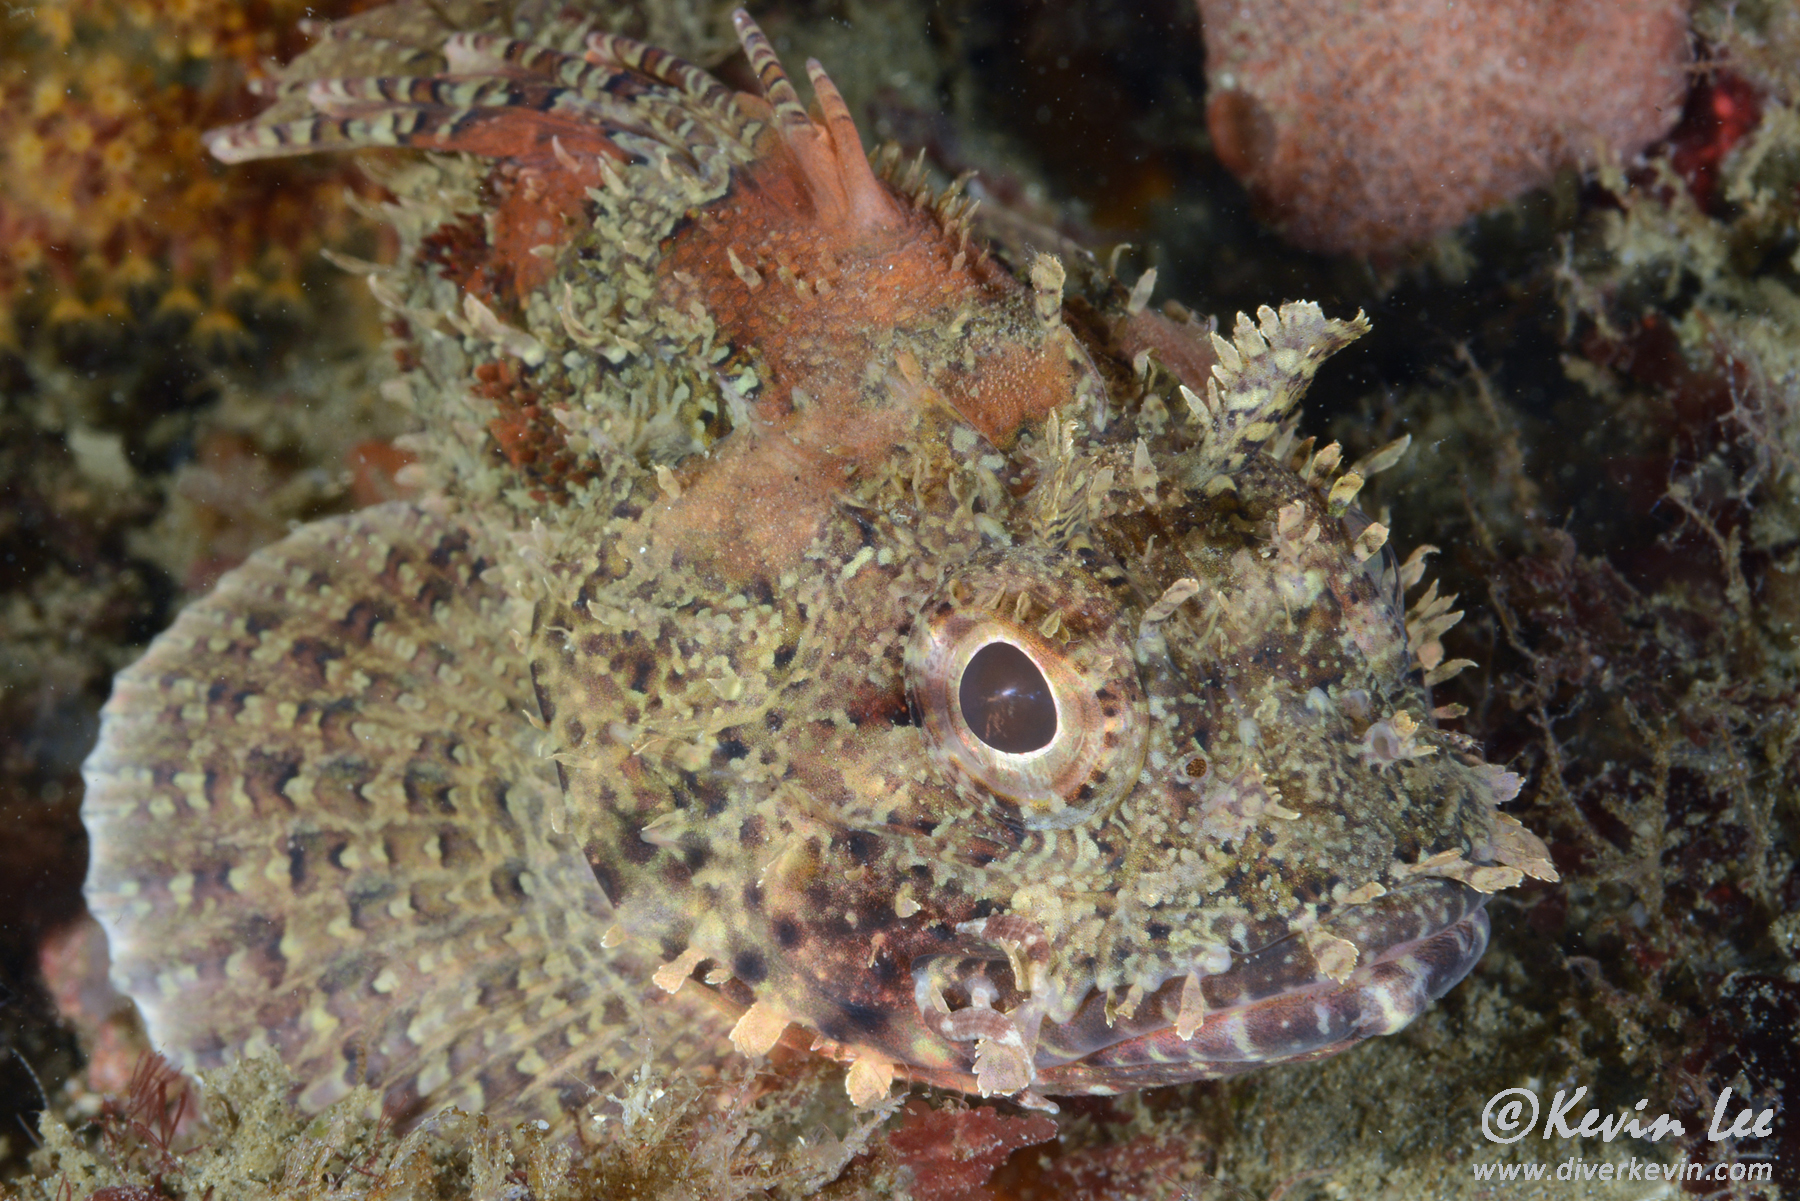
\includegraphics[width=.5\textwidth]{cover_photo}

\end{frame}

\begin{frame}{Early Life History}

\begin{itemize} 
\item[$\bullet$] Migration to spawning grounds, exhibit explosive breeding behavior just before dawn
\item[$\bullet$] External fertilization, females produce hollow gelatenous single-layer floating egg matrix
\item[$\bullet$] Eggs hatch after about 5 days
\item[$\bullet$] Juveniles settle at less than 2 cm 
\end{itemize}

\centering
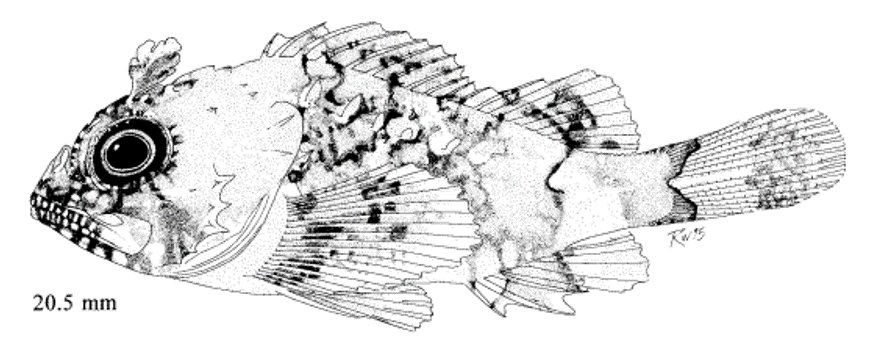
\includegraphics[width=.5\textwidth]{Figures/baby_scorp}

\footnotetext{Line drawning from CalCOFI Atlas 33, pg. 789 Figure 26}

\end{frame}

\begin{frame}{Distribution and Stock Assessment Boundary}

\begincols
 \begincol{.5\textwidth} 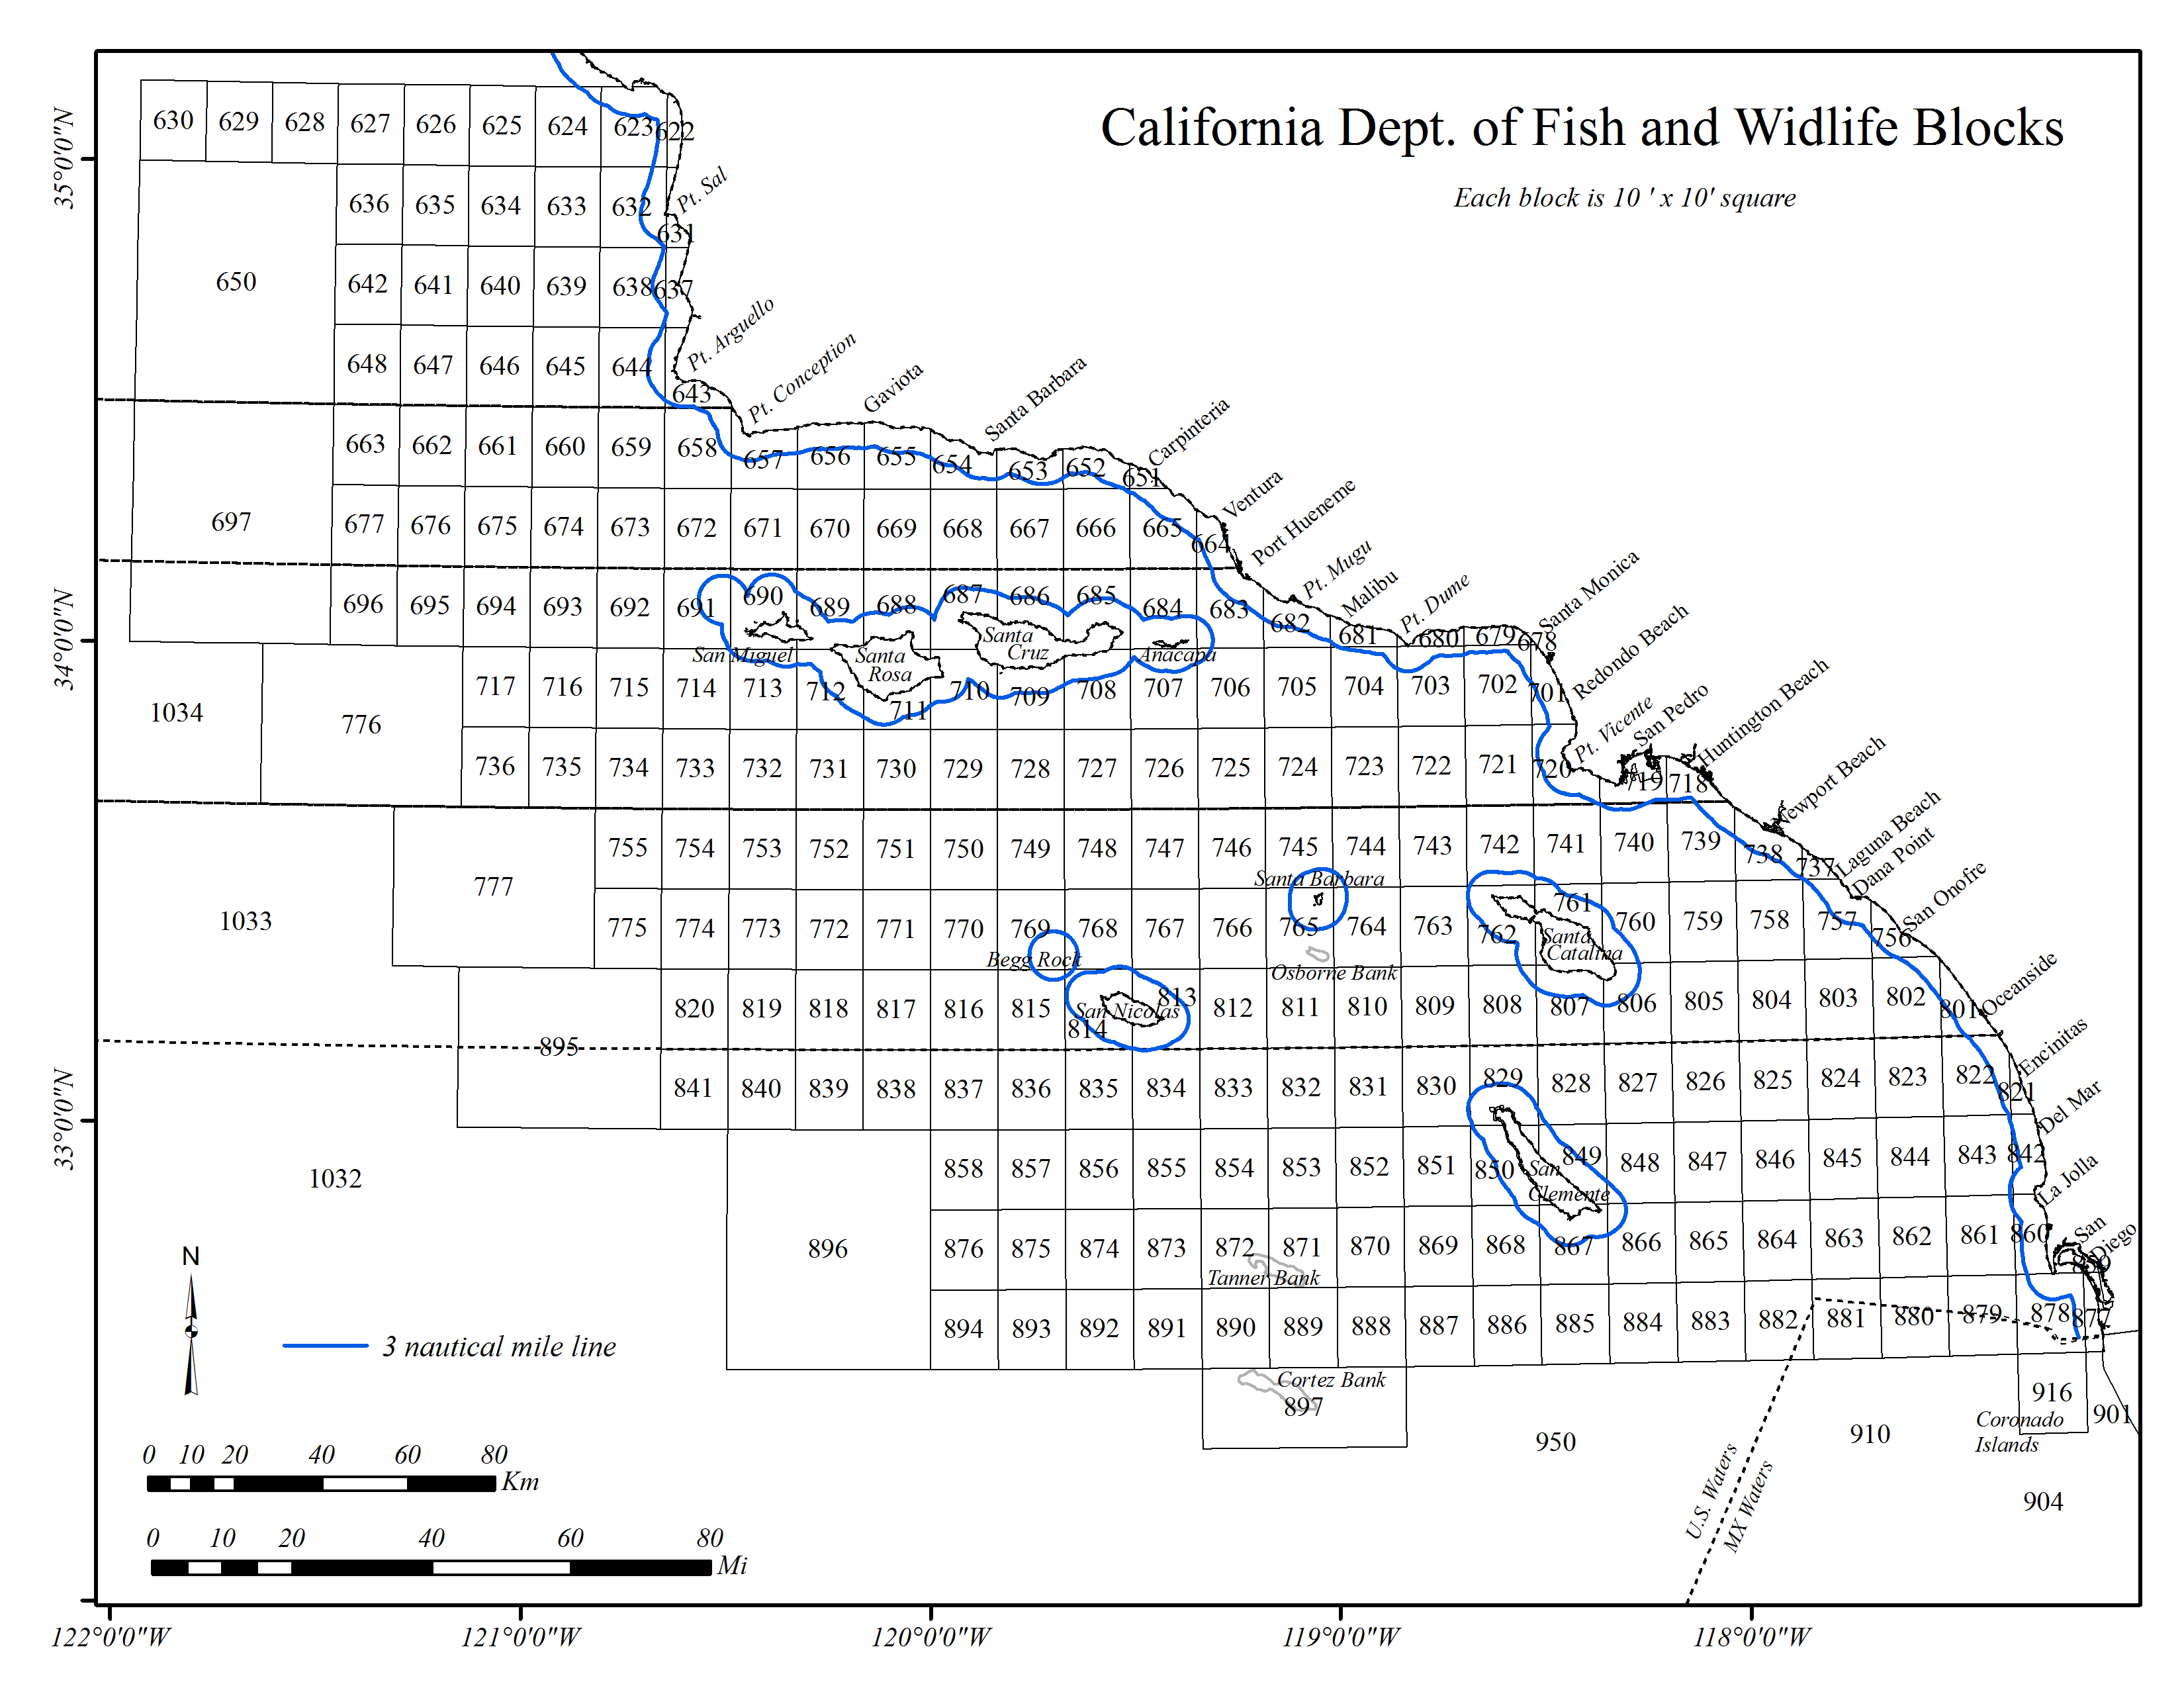
\includegraphics{Figures/assess_region_map.png}

\endcol
 \begincol{.5\textwidth}

\begin{itemize} 
 \item[$\bullet$] Distributed from central California to Punta Eugenia, Baja California Sur, Mexico 
 \item[$\bullet$] Assessment south of Pt. Conception to U.S/Mexico border 
 \item[$\bullet$] Observed from the intertidal to 600 ft,  prefer depths of 20-450 ft  
 \item[$\bullet$] Proportion of the stock in Mexican waters unknown
\end{itemize}

\endcol
\endcols

\end{frame}

\begin{frame}{2005 Stock Assessment}

\begin{itemize}
\item[$\bullet$] Transitioning from the 2005 assessment, an error was found
\item[$\bullet$] Harvest rate hit the bounds for the recreational fleet
\item[$\bullet$] Not all of the recreational catch was removed in the model
\item[$\bullet$] Input vs. estimated catch was not standard output in SS v.1.8
\end{itemize}

\begincols
 \begincol{.5\textwidth}

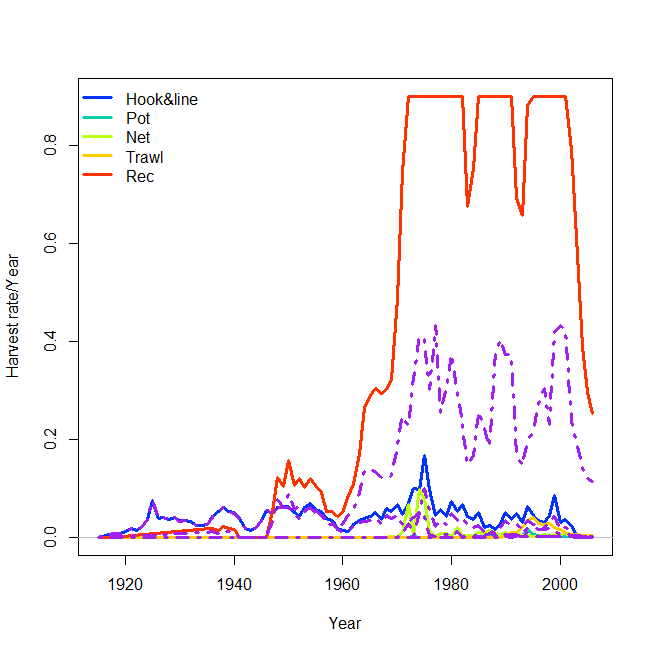
\includegraphics{Figures/bridge_harvestrate.png}

\endcol
 \begincol{.5\textwidth}

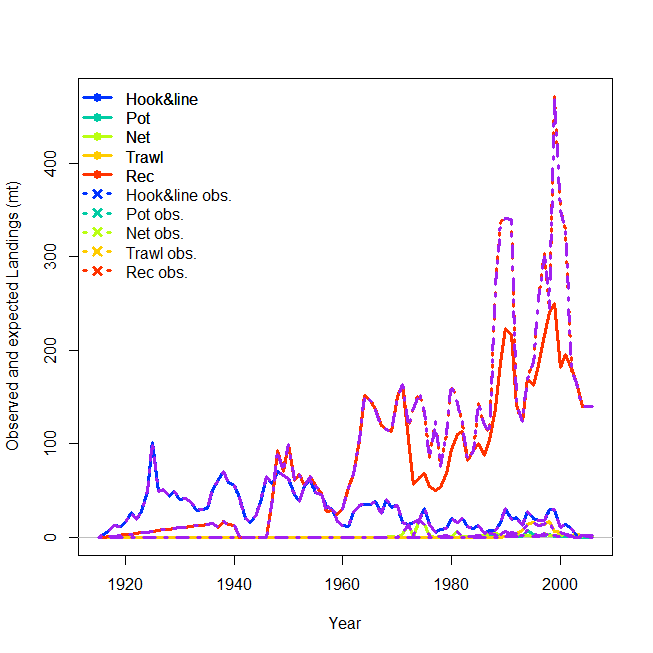
\includegraphics{Figures/bridge_catch.png}

\endcol
\endcols

\end{frame}

\begin{frame}{2005 Stock Assessment}

\begincols
 \begincol{.5\textwidth}

\begin{itemize}
\item[$\bullet$] \textcolor{blue}{2005 assessment, SS v.1.8}
\item[$\bullet$] \textcolor{red}{2005 model in SS3.24z}
\item[$\bullet$] \textcolor{violet}{2017 pre-STAR base model, SS3.30.0.05}
\item[$\bullet$] The two assessments have very similar trends over time, with $B_0$ higher for the 2017 assessment that includes all removals
\end{itemize}

\endcol
 \begincol{.5\textwidth}

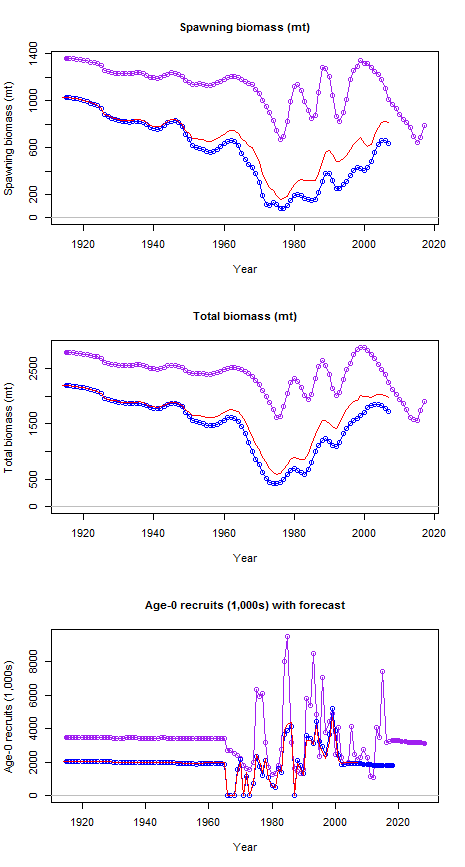
\includegraphics{Figures/bridge_timeseries.png}

\endcol
\endcols

\end{frame}

\begin{frame}{2017 Stock Assessment}

Pre-STAR Base Model

\begin{itemize}
\item[$\bullet$] One area south of Pt. Conception 
\begin{itemize}
\item[$\circ$] Catches from Mexican waters excluded as in 2005
\end{itemize}
\item[$\bullet$] Steepness fixed at 0.718
\item[$\bullet$] Sex-specific $M$ fixed for females, male $M$ estimated as offset
\item[$\bullet$] Re-evaluated fleet definitions
\item[$\bullet$] Ages now available from the NWFSC trawl survey
\item[$\bullet$] New indices and length compositions available
\item[$\bullet$] Newest version of SS allows specification of the minimmum sample size
\end{itemize}

\end{frame}

\section{Catch}\label{catch}

\begin{frame}{Catches by Fleet}

\centering
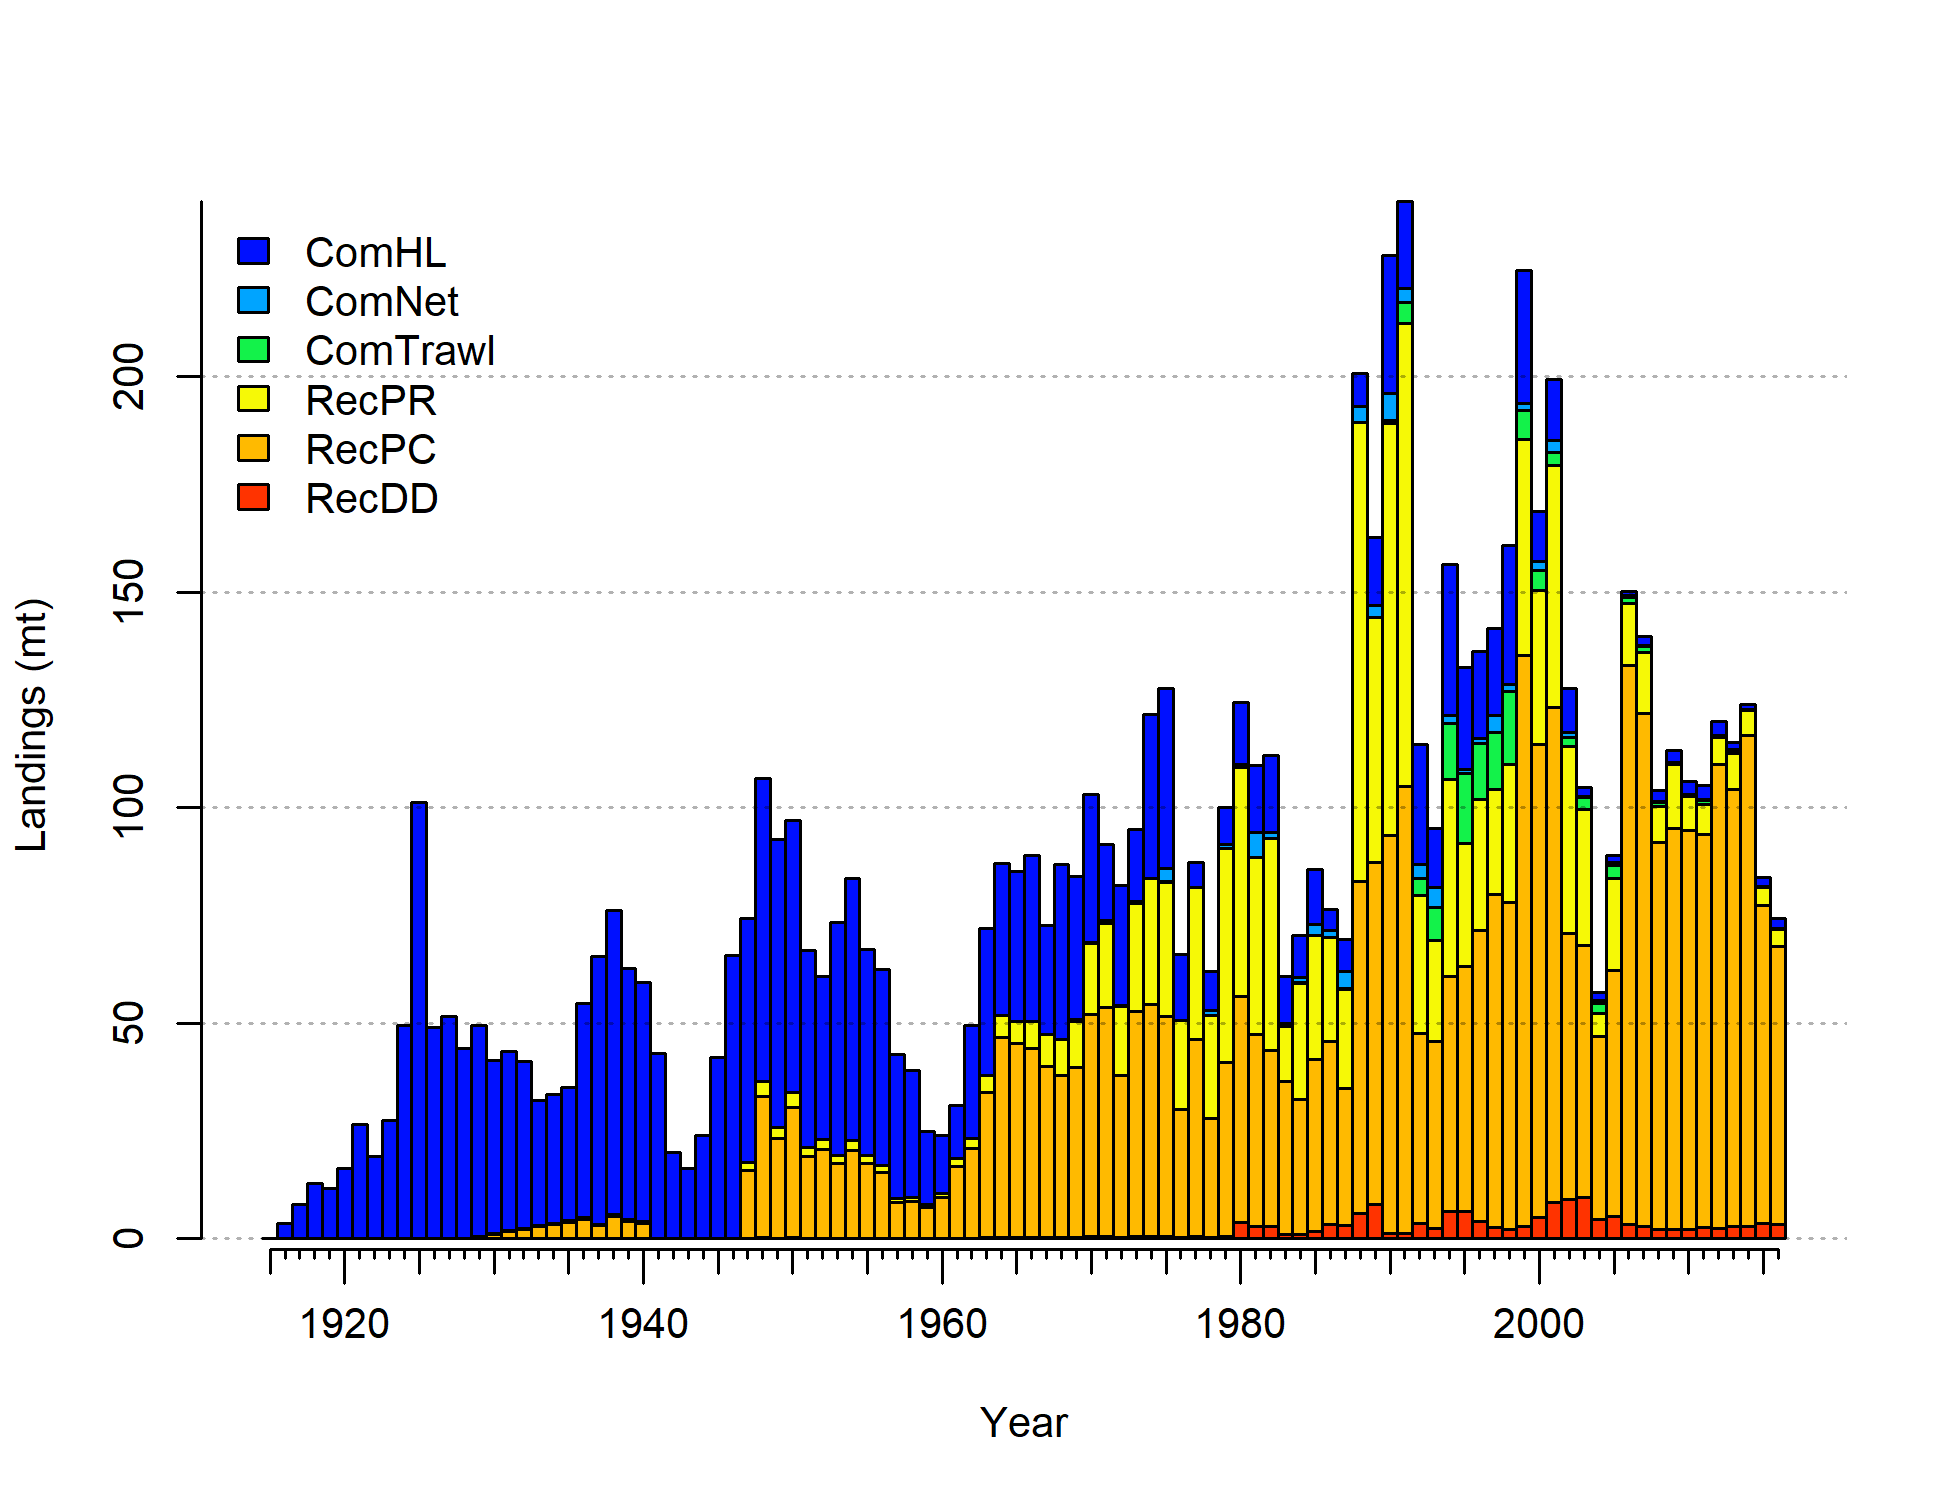
\includegraphics{r4ss/plots_mod1/catch2 landings stacked.png}

\end{frame}

\begin{frame}{Recreational Catch}

\begincols
 \begincol{.4\textwidth}

\begin{itemize}
\item[$\bullet$] 2005 assessment used number of fish for recreational catches
\item[$\bullet$] 2017 assessment includes one recreational discard fleet
\begin{itemize}
\item[$\circ$] Discard mortality rate of 7\%
\item[$\circ$] Discard biomass accounts for  $<$3\% of recreational mortality
\end{itemize}
\end{itemize}

\endcol
 \begincol{.6\textwidth}
\includegraphics[totalheight=0.65\textheight]{California_scorpionfish_2017_files/figure-latex/unnamed-chunk-16-1.pdf}\\
\endcol
\endcols

\end{frame}

\begin{frame}{Commercial Catch}

\begincols
 \begincol{.4\textwidth}

\begin{itemize}
  \item[$\bullet$] Historical catches same as the 2005 assessment
  \item[$\bullet$] California Fisheries Information System (CFIS) landings data used to update catches from 2005-2016 
  \item[$\bullet$] Discards assumed neglible
\end{itemize}

\endcol
 \begincol{.55\textwidth}
\includegraphics{California_scorpionfish_2017_files/figure-latex/unnamed-chunk-17-1.pdf}
\endcol
\endcols

\end{frame}

\section{Indices}\label{indices}

\begin{frame}{Indices of Abundance}

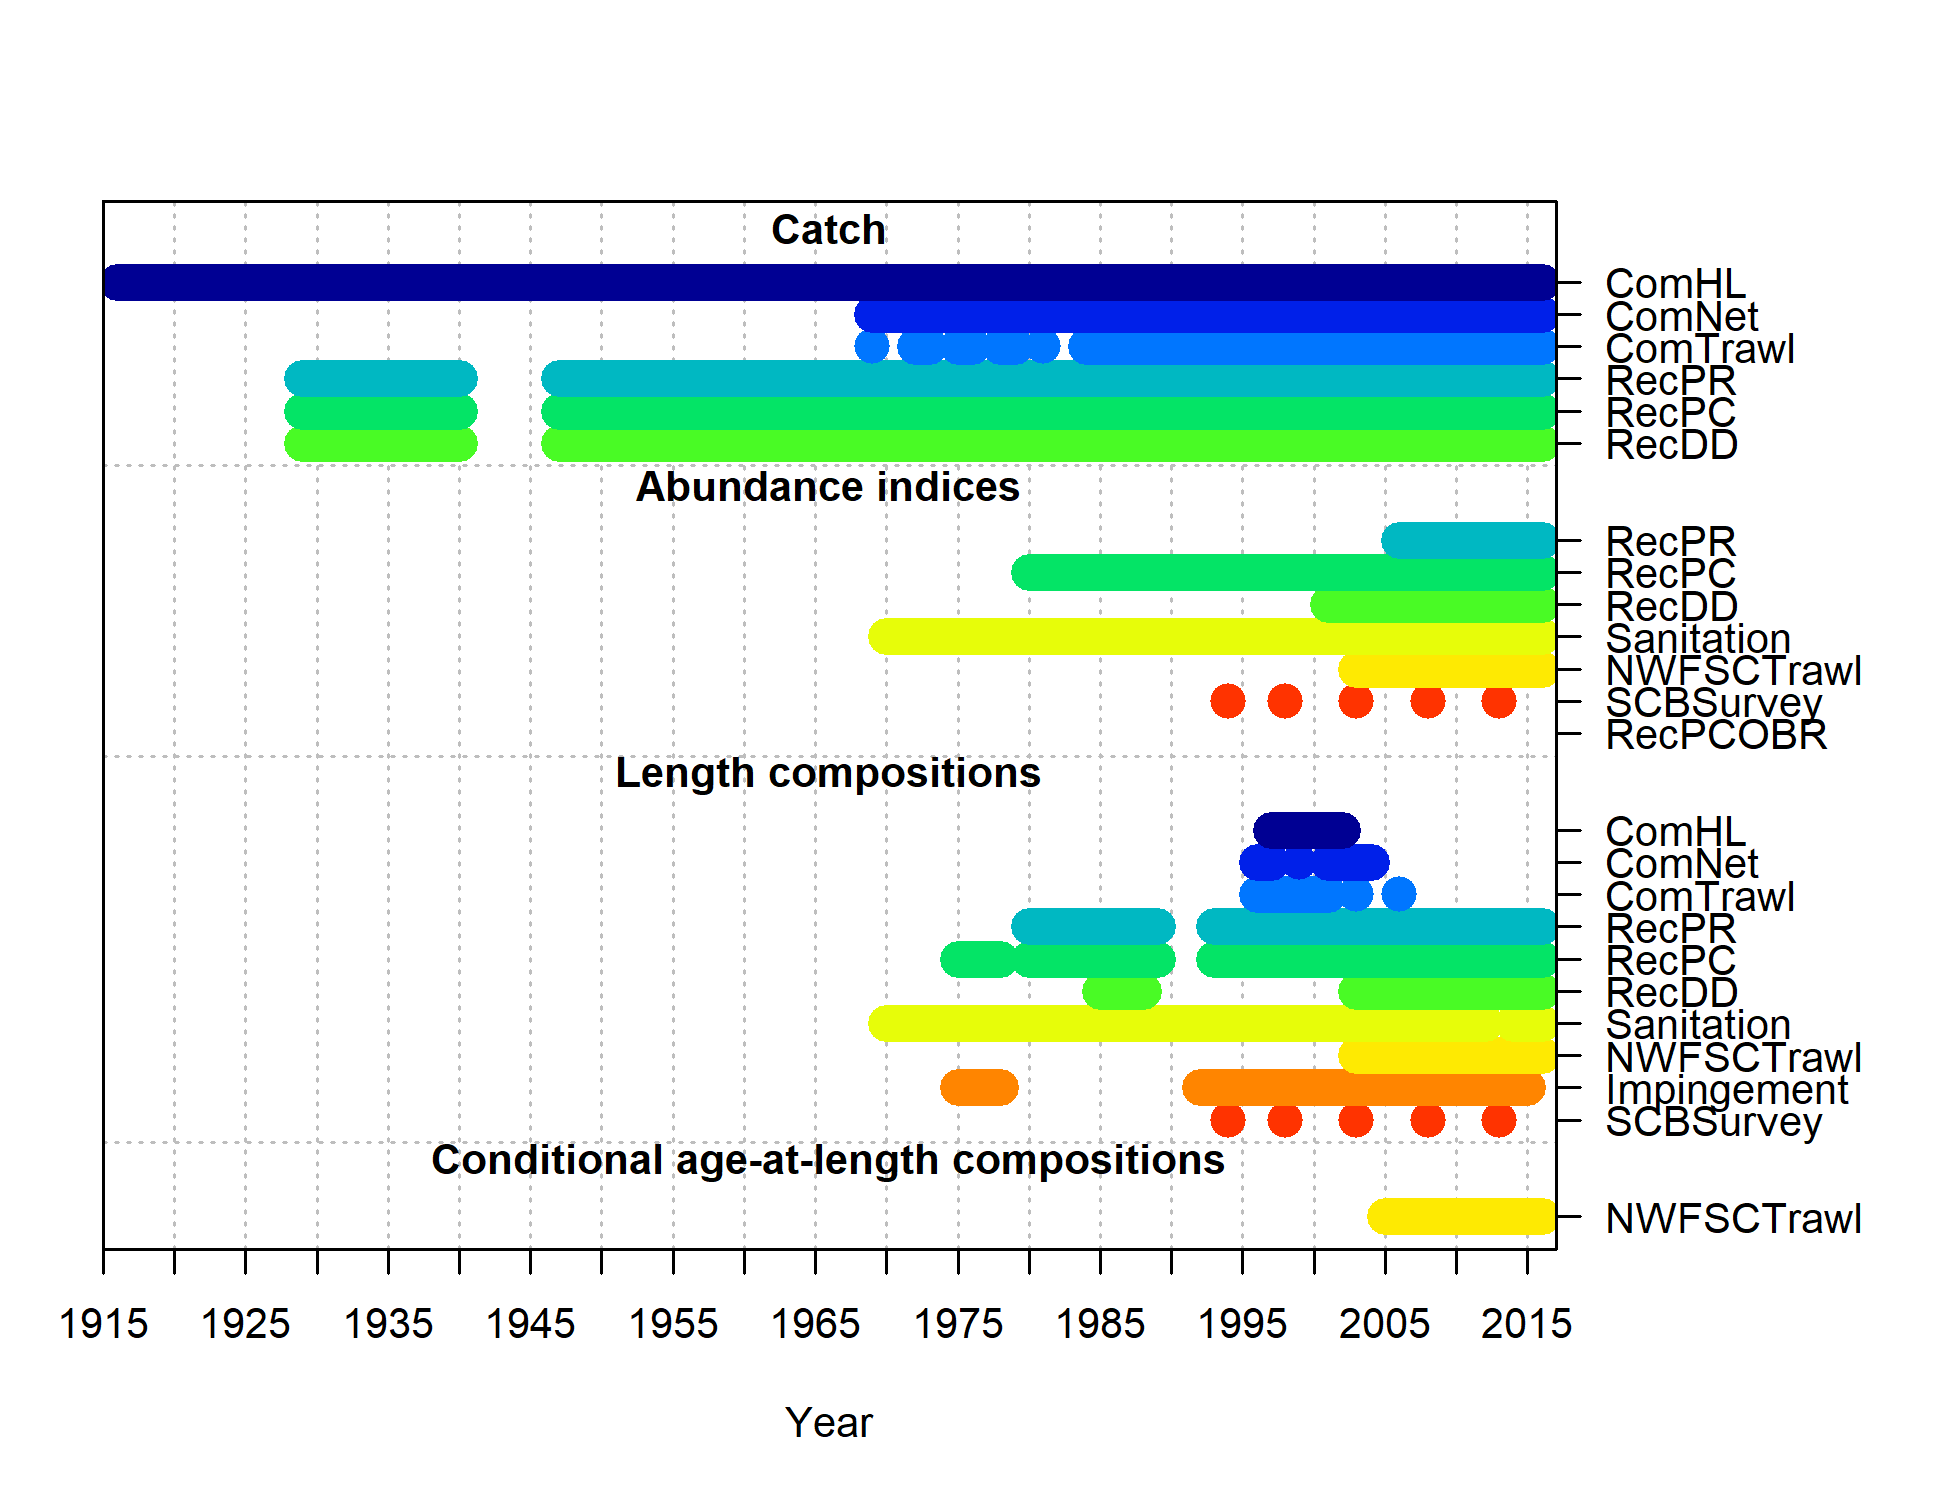
\includegraphics{r4ss/plots_mod1/data_plot.png}

\end{frame}

\begin{frame}{Indices of Abundance}

\begin{itemize}
\tightlist
\item
  All of the methods used to standardize indices have been endorsed by
  the SSC
\end{itemize}

\begin{table}[ht]
\centering
\scalebox{0.7}{
\begin{tabular}{p{2.5in}p{0.8in}p{.4in}p{2in}}
  \hline
Name & Years & Fishery ind. & Method \\ 
  \hline
Recreational PR dockside CPUE & 2004-2016 & No & delta-GLM (bin-lognormal) \\ 
  CPFV logbook CPUE & 1980-2016 & No & negative binomial \\ 
  Onboard observer discard catch CPUE & 2002-2016 & No & delta-GLM (bin-lognormal) \\ 
  Sanitation district CPUE & 1970-2016 & Yes & delta-GLM (bin-lognormal) \\ 
  NWFSC trawl survey CPUE & 2003-2016 & Yes & VAST \\ 
  CSUN/VRG Gillnet survey CPUE & 1995-2008 & Yes & delta-GLM (bin-lognormal) \\ 
  Southern California Bight trawl survey CPUE & '94, '98, '03, '08, '13 & Yes & delta-GLM (bin-lognormal) \\ 
  Onboard observer retained catch CPUE & 2002-2016 & No & delta-GLM (bin-lognormal) \\ 
   \hline
\end{tabular}
}
\end{table}

\end{frame}

\begin{frame}{Indices of Abundance}

\end{frame}

\section{Composition}\label{composition}

\begin{frame}{Length compositions were provided from the following
sources:}

\begin{itemize}
  \item[$\bullet$] CDFW market category study (\emph{commercial dead fish}, 1996-2003)    
  \item[$\bullet$] CALCOM (\emph{commercial dead fish}, 2013-2016)    
  \item[$\bullet$] CDFW onboard observer (\emph{recreational charter discards}, 2003-2016)  
  \item[$\bullet$] Collins and Crooke onboard observer surveys (1975-1978) 
  \item[$\bullet$] Ally onboard observer study (\emph{recreational charter kept/discards}, 1984-1989)  
  \item[$\bullet$] MRFSS (1980-2003) and CRFS (2004-2014) (\emph{private and party/charter, kept})
  \item[$\bullet$] POTW trawl surveys (\emph{research}, 1970-2016)      
  \item[$\bullet$] CSUN/VRG gillnet survey (\emph{research}, 1995-2008)        
  \item[$\bullet$] Power plant impingement surveys (\emph{research}, 1974-2016)  
  \item[$\bullet$] Southern California Bight trawl survey (\emph{research}, 1994, 1998, 2003, 2008, 2013) 
\end{itemize}

\end{frame}

\begin{frame}{Aggregate length composition}

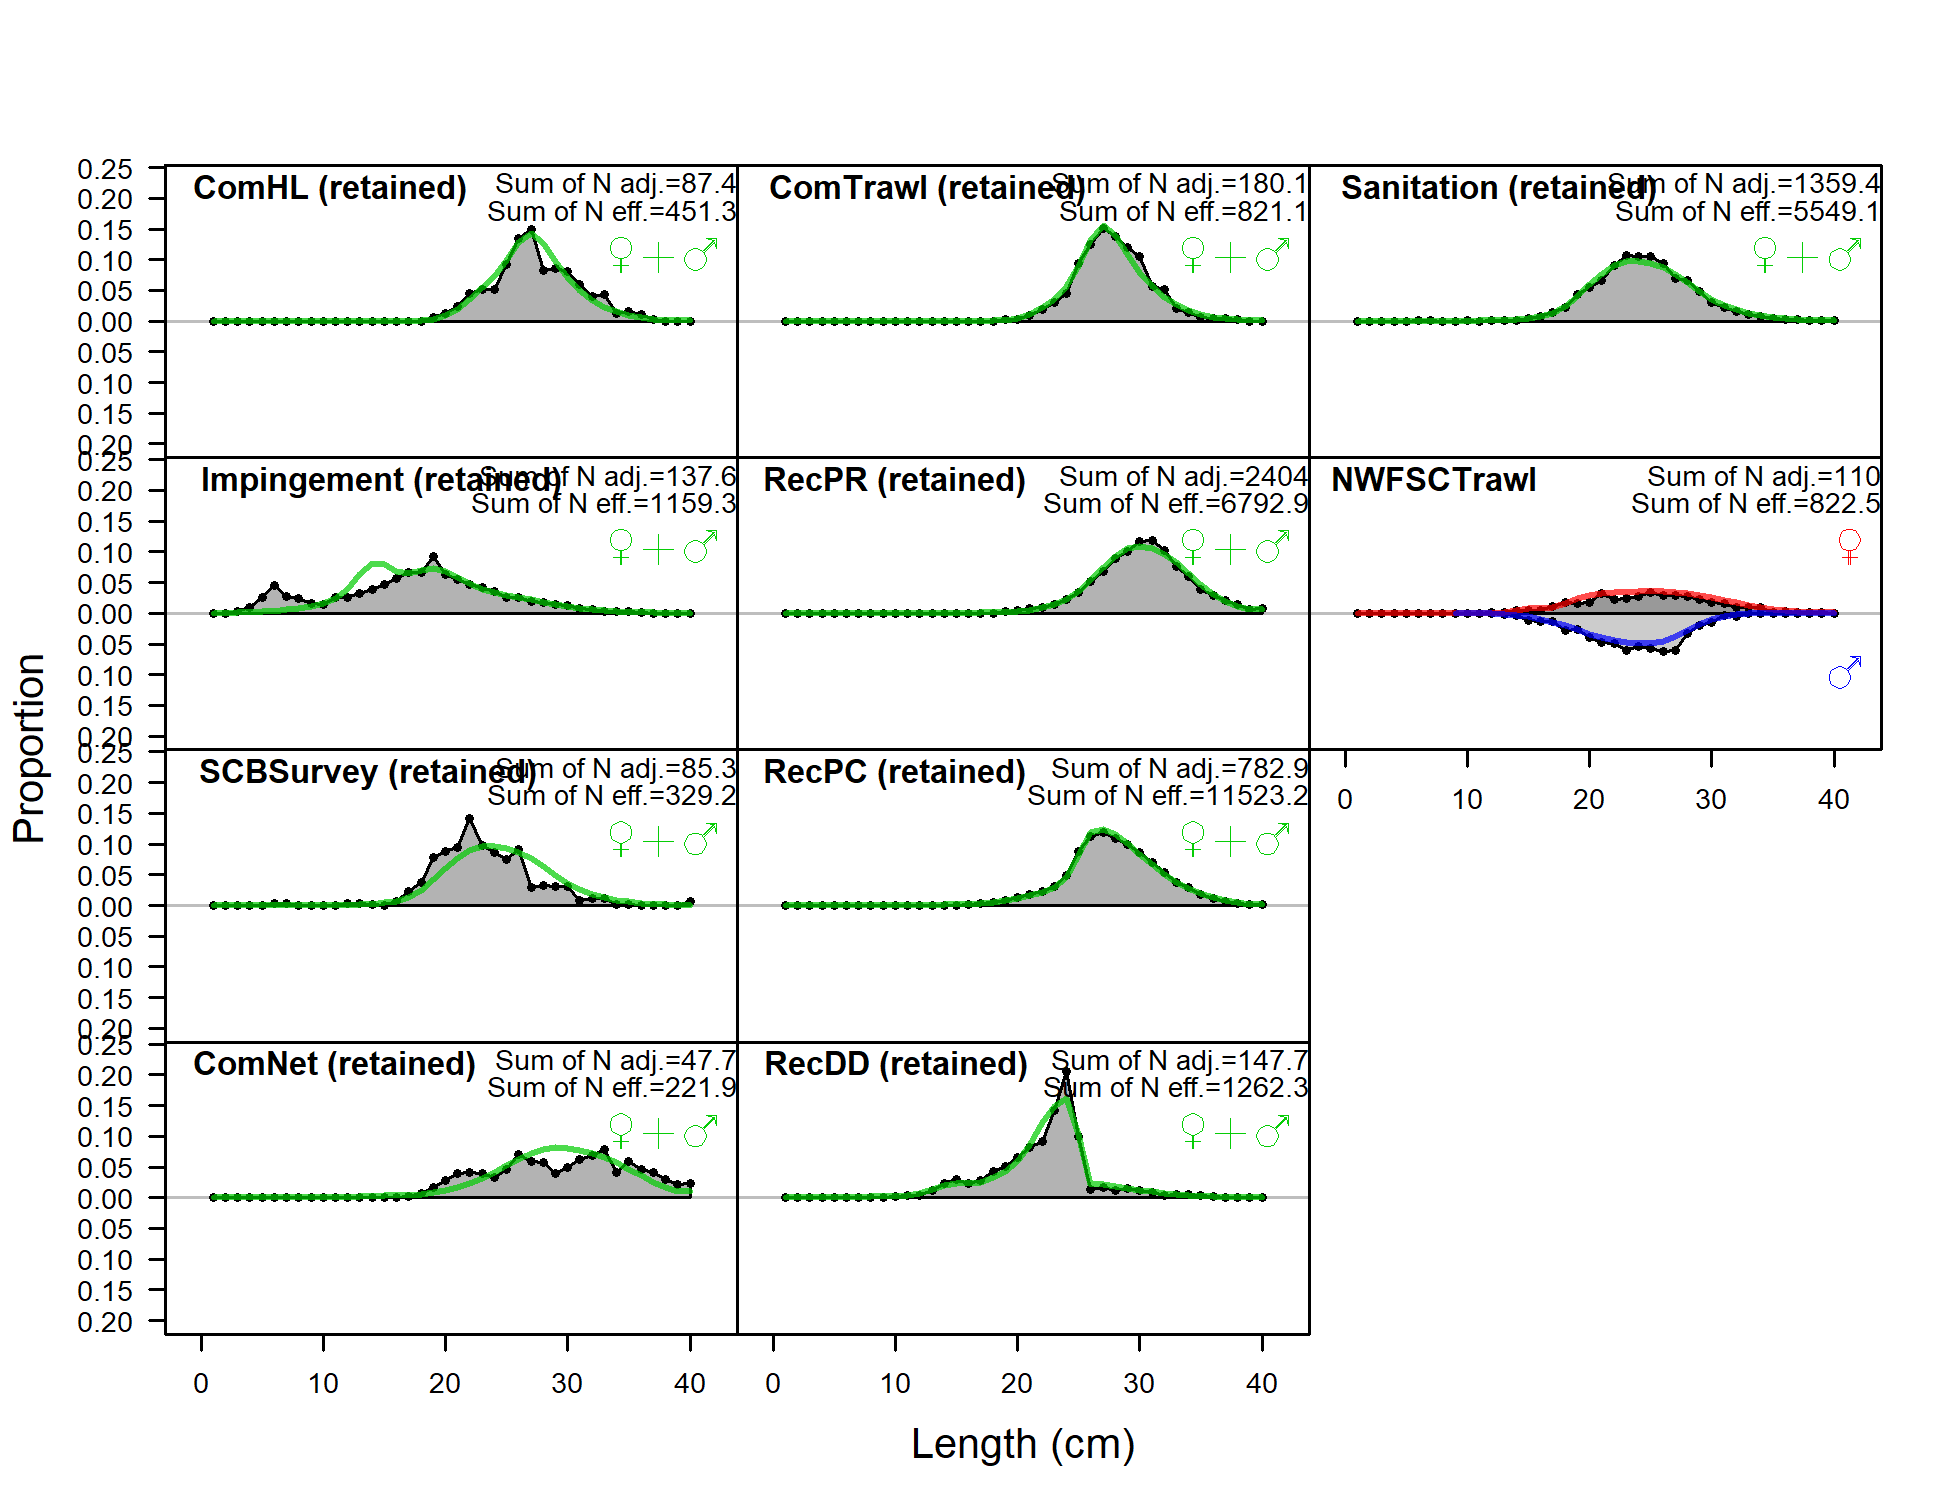
\includegraphics{r4ss/plots_mod1/comp_lenfit__aggregated_across_time.png}

\end{frame}

\begin{frame}{Commercial fishery length composition}

\begincols
 \begincol{.5\textwidth} \centering
 Commercial hook-and-line
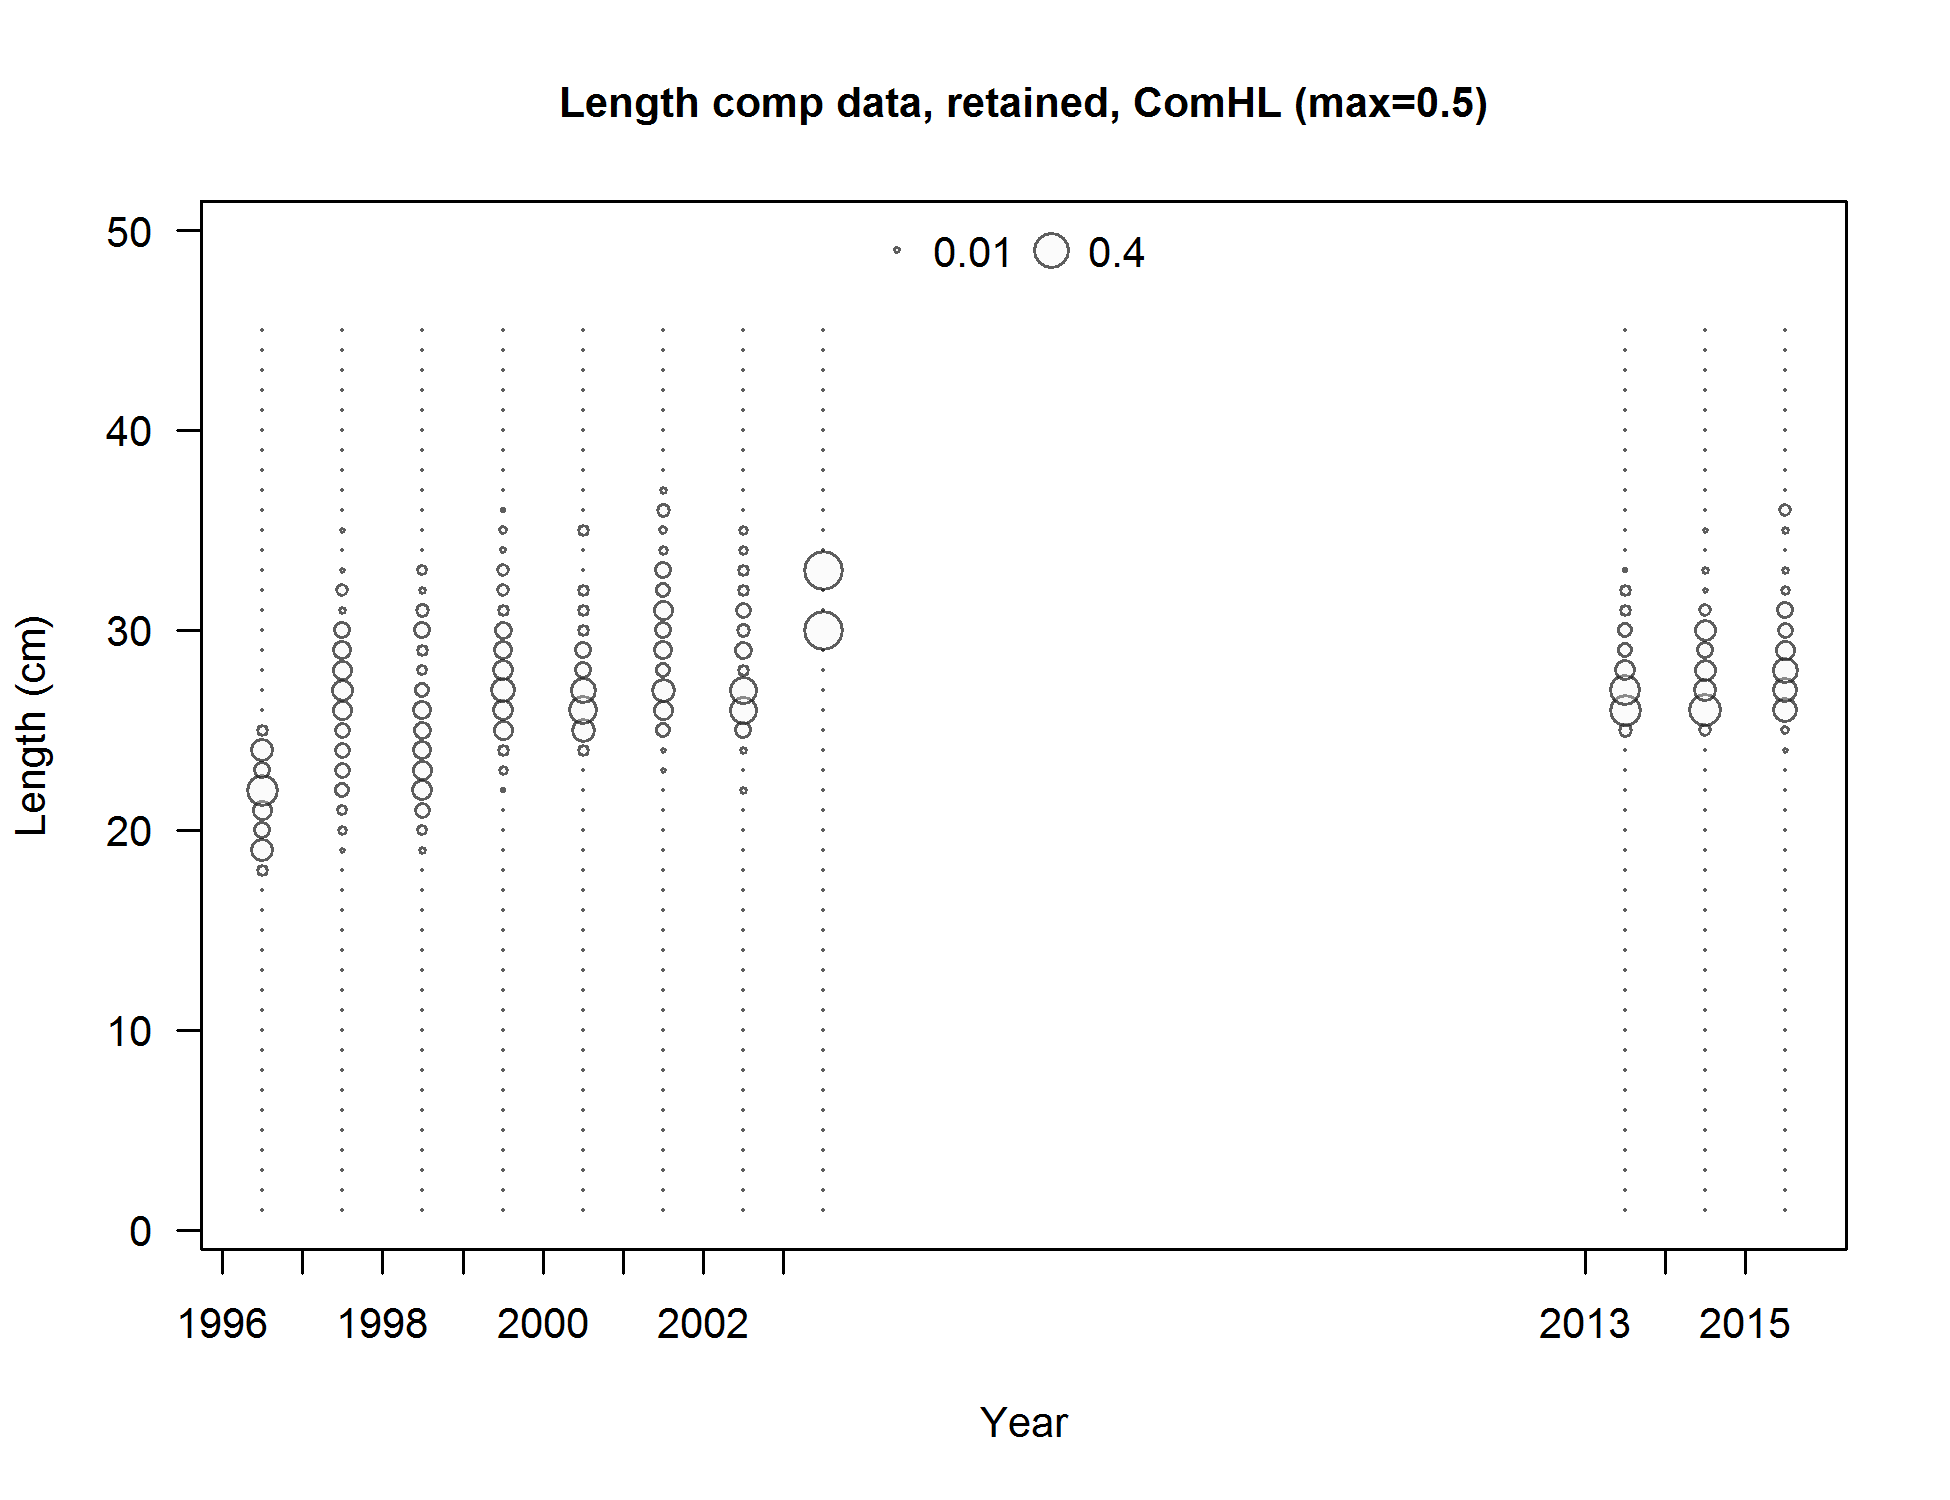
\includegraphics[height=3cm]{r4ss/plots_mod1/comp_lendat_bubflt1mkt2.png}

Commercial gillnet
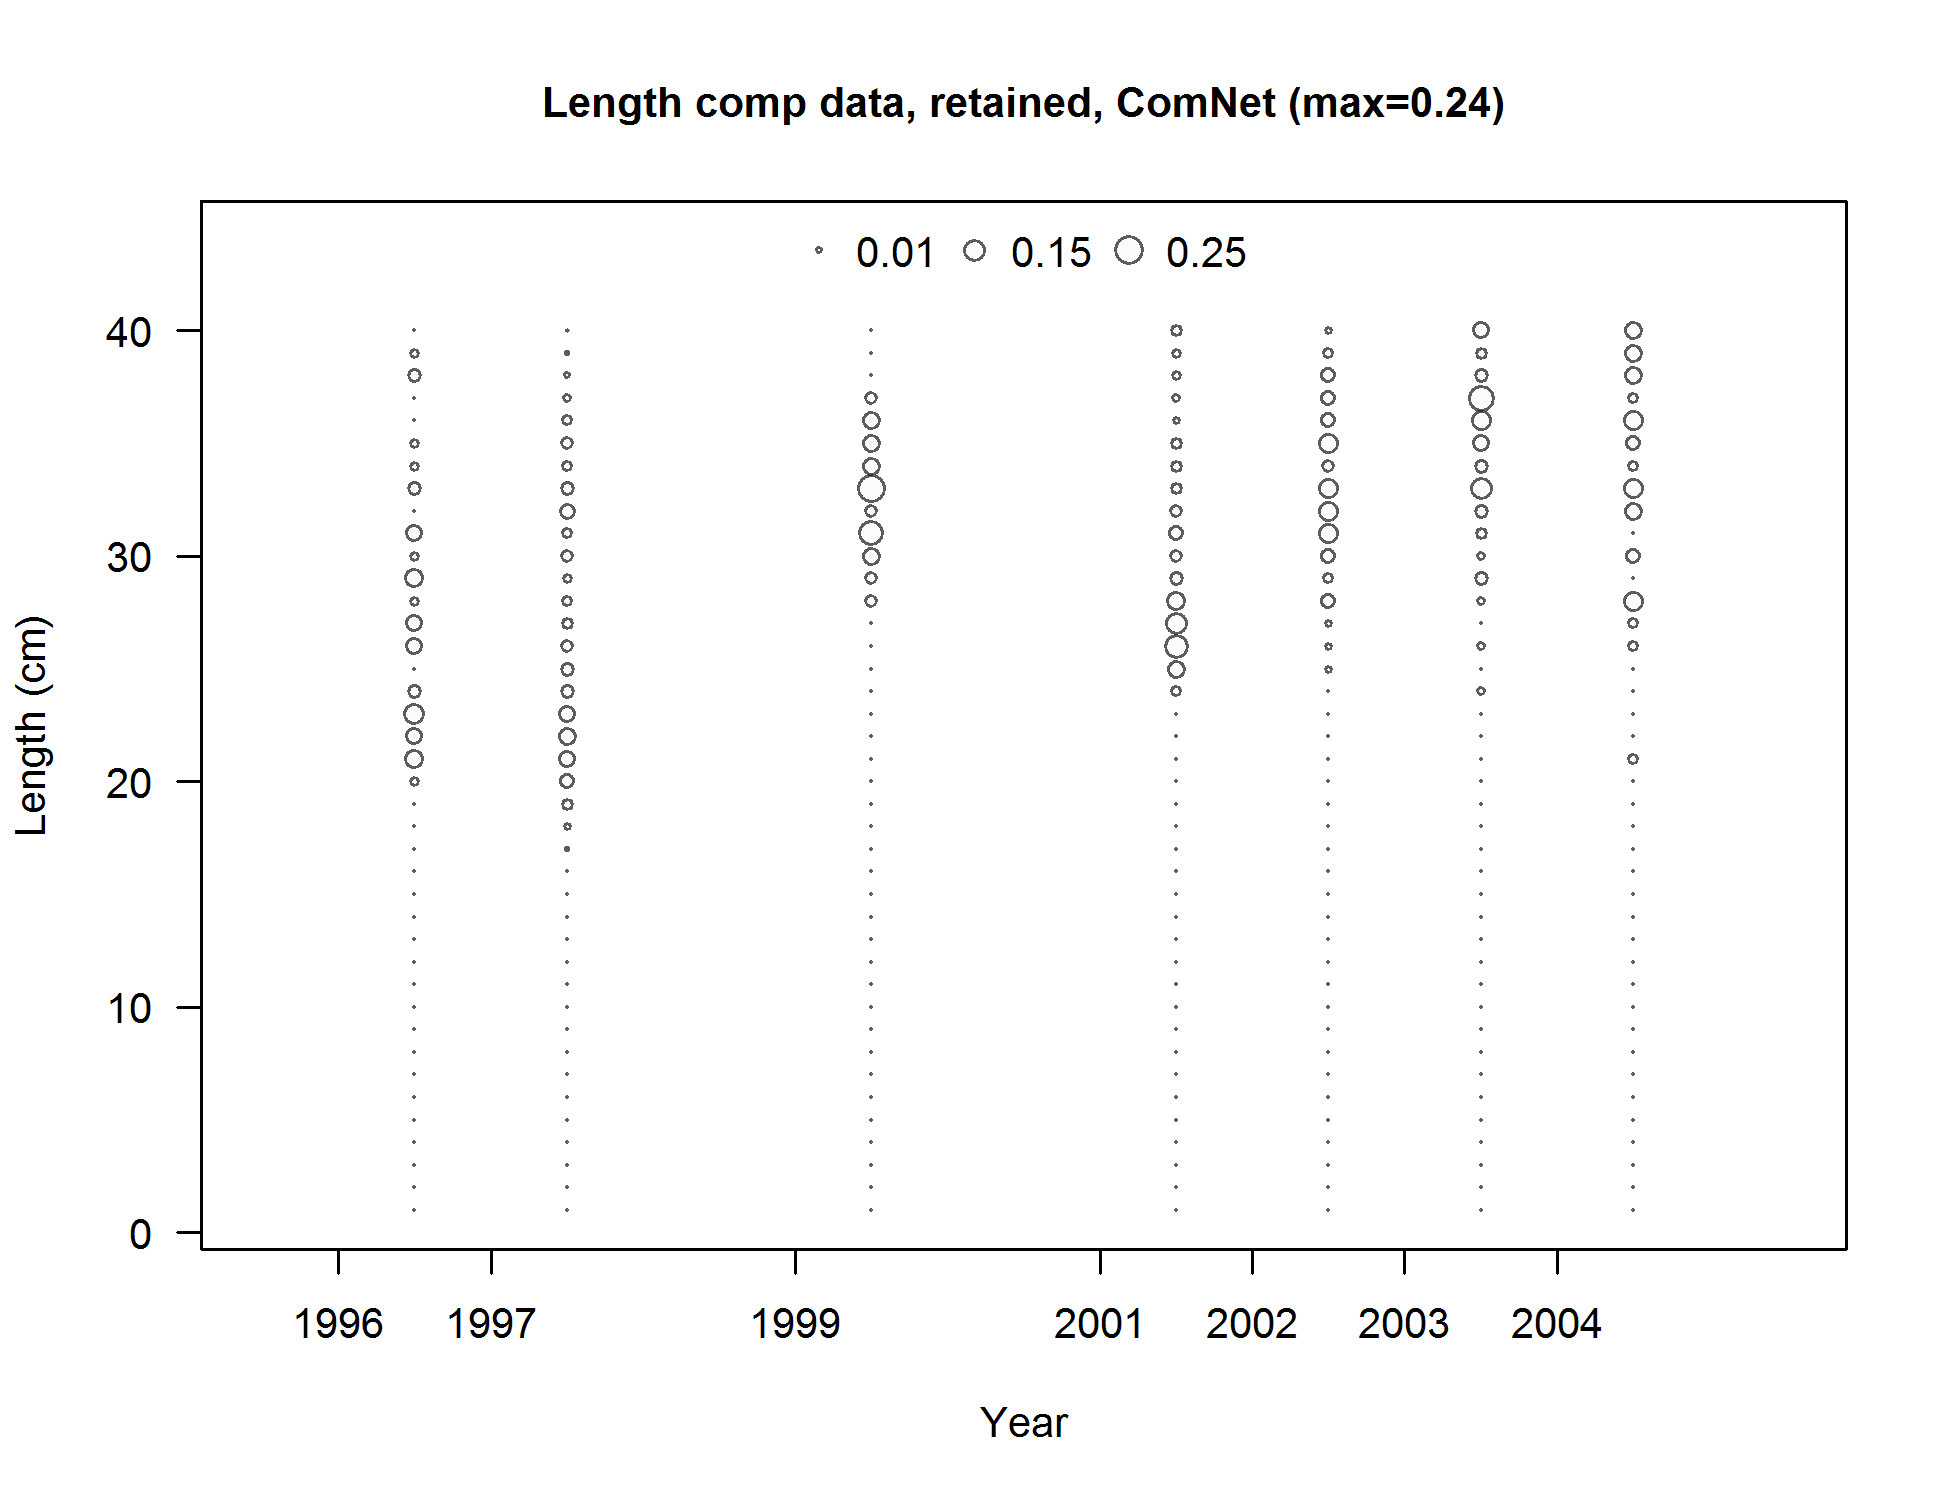
\includegraphics[height=3cm]{r4ss/plots_mod1/comp_lendat_bubflt2mkt2.png}
\endcol
 \begincol{.5\textwidth} \centering
 Commercial trawl
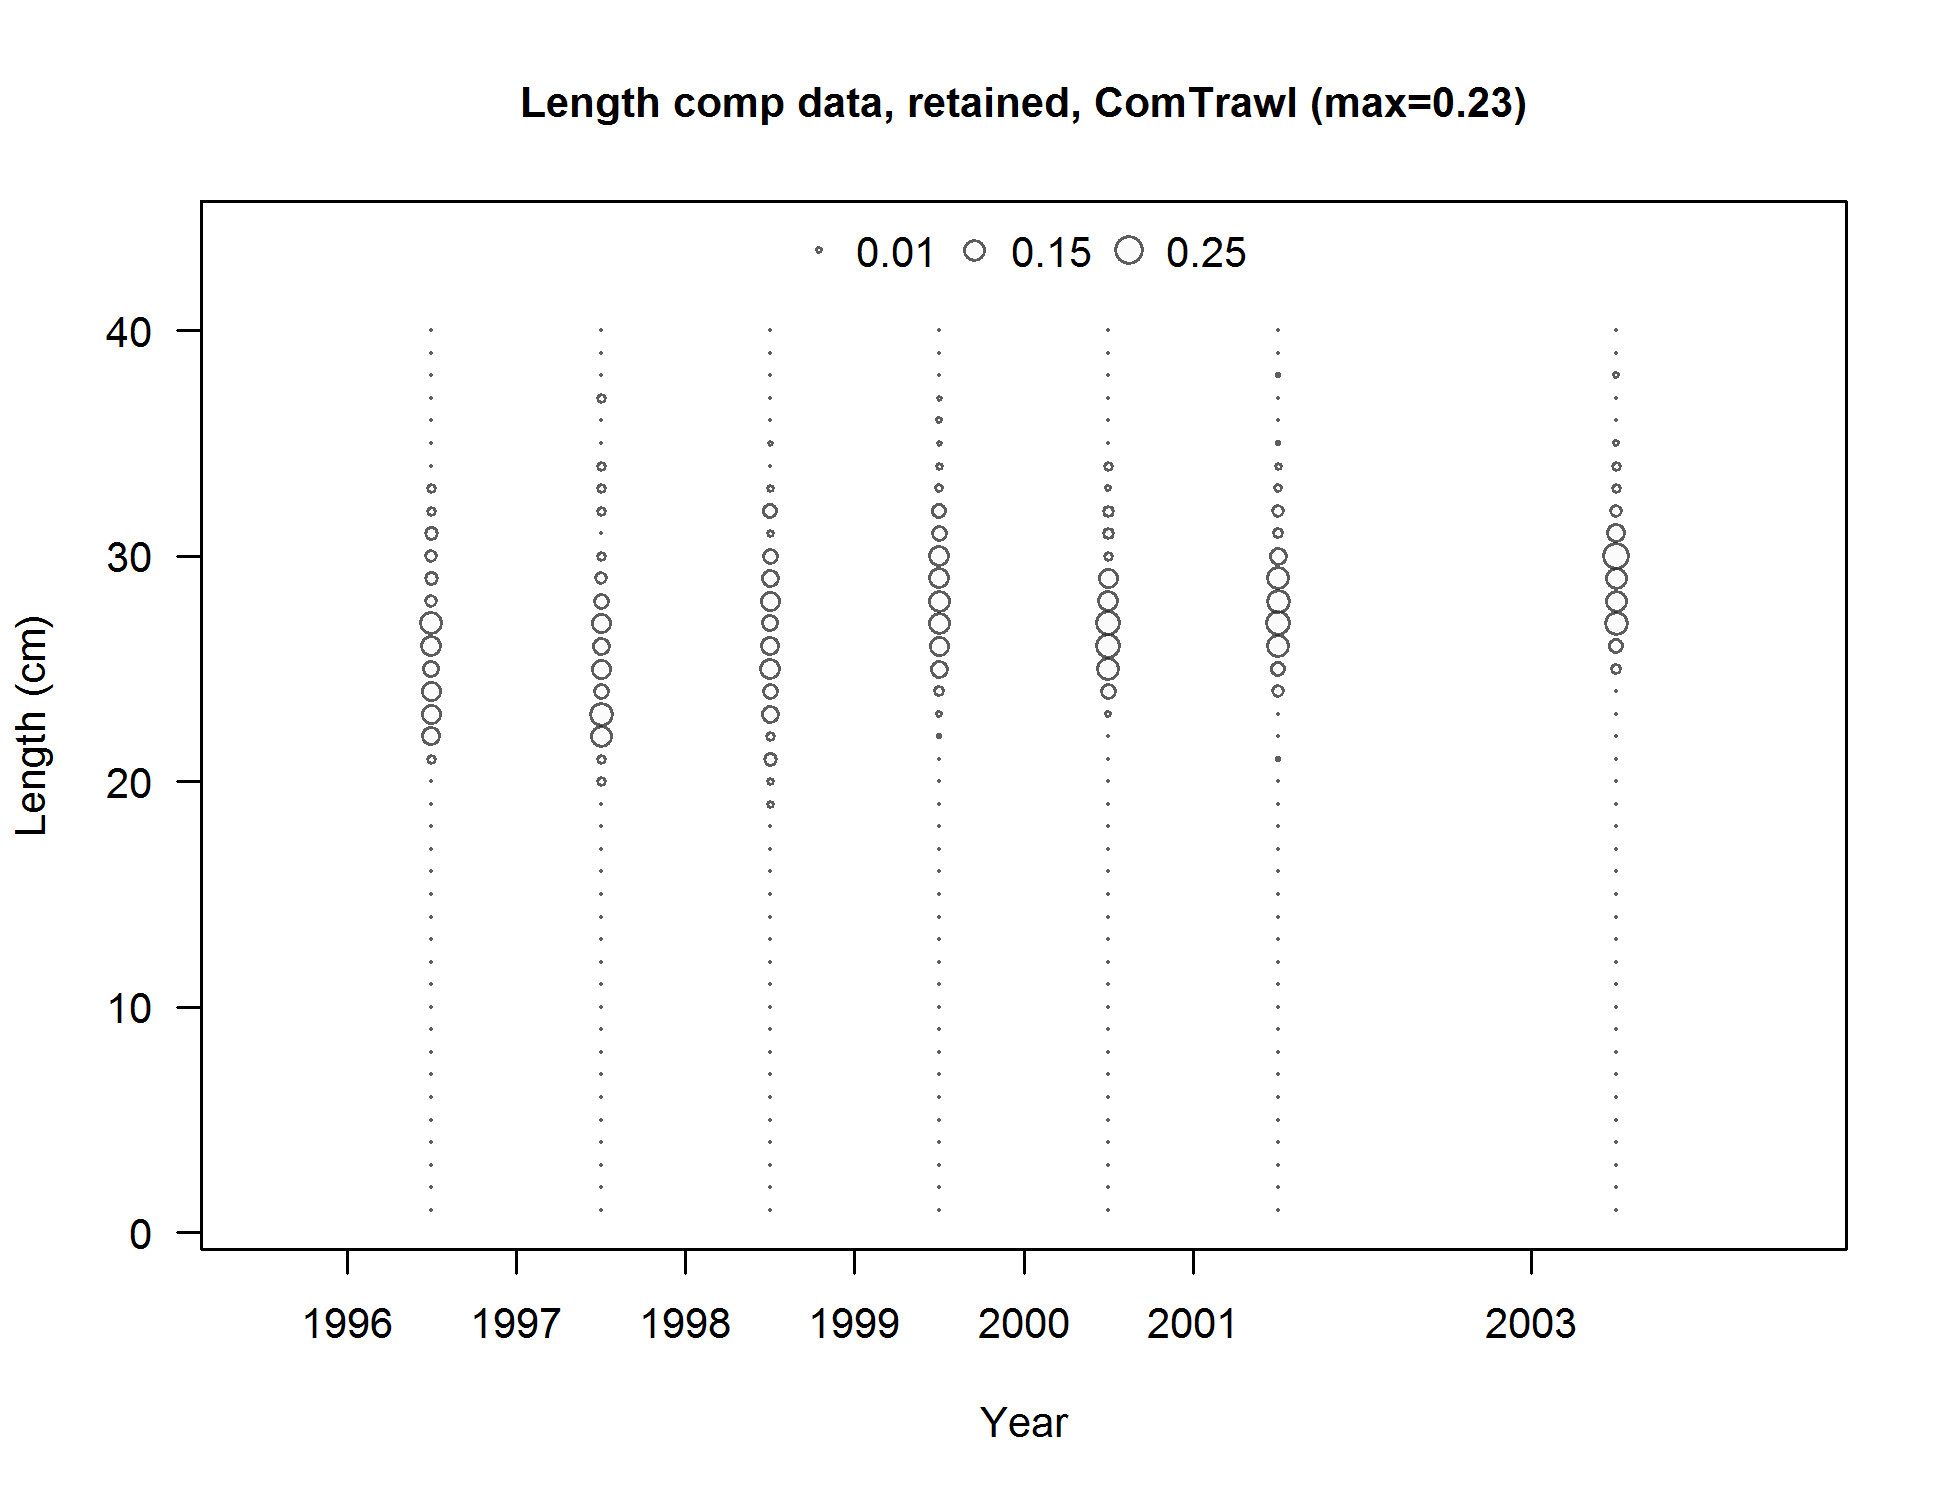
\includegraphics[height=4cm]{r4ss/plots_mod1/comp_lendat_bubflt3mkt2.png}
\endcol
\endcols

\end{frame}

\begin{frame}{Recreational fishery Length Composition}

\begincols
 \begincol{.5\textwidth} Recreational private fleet
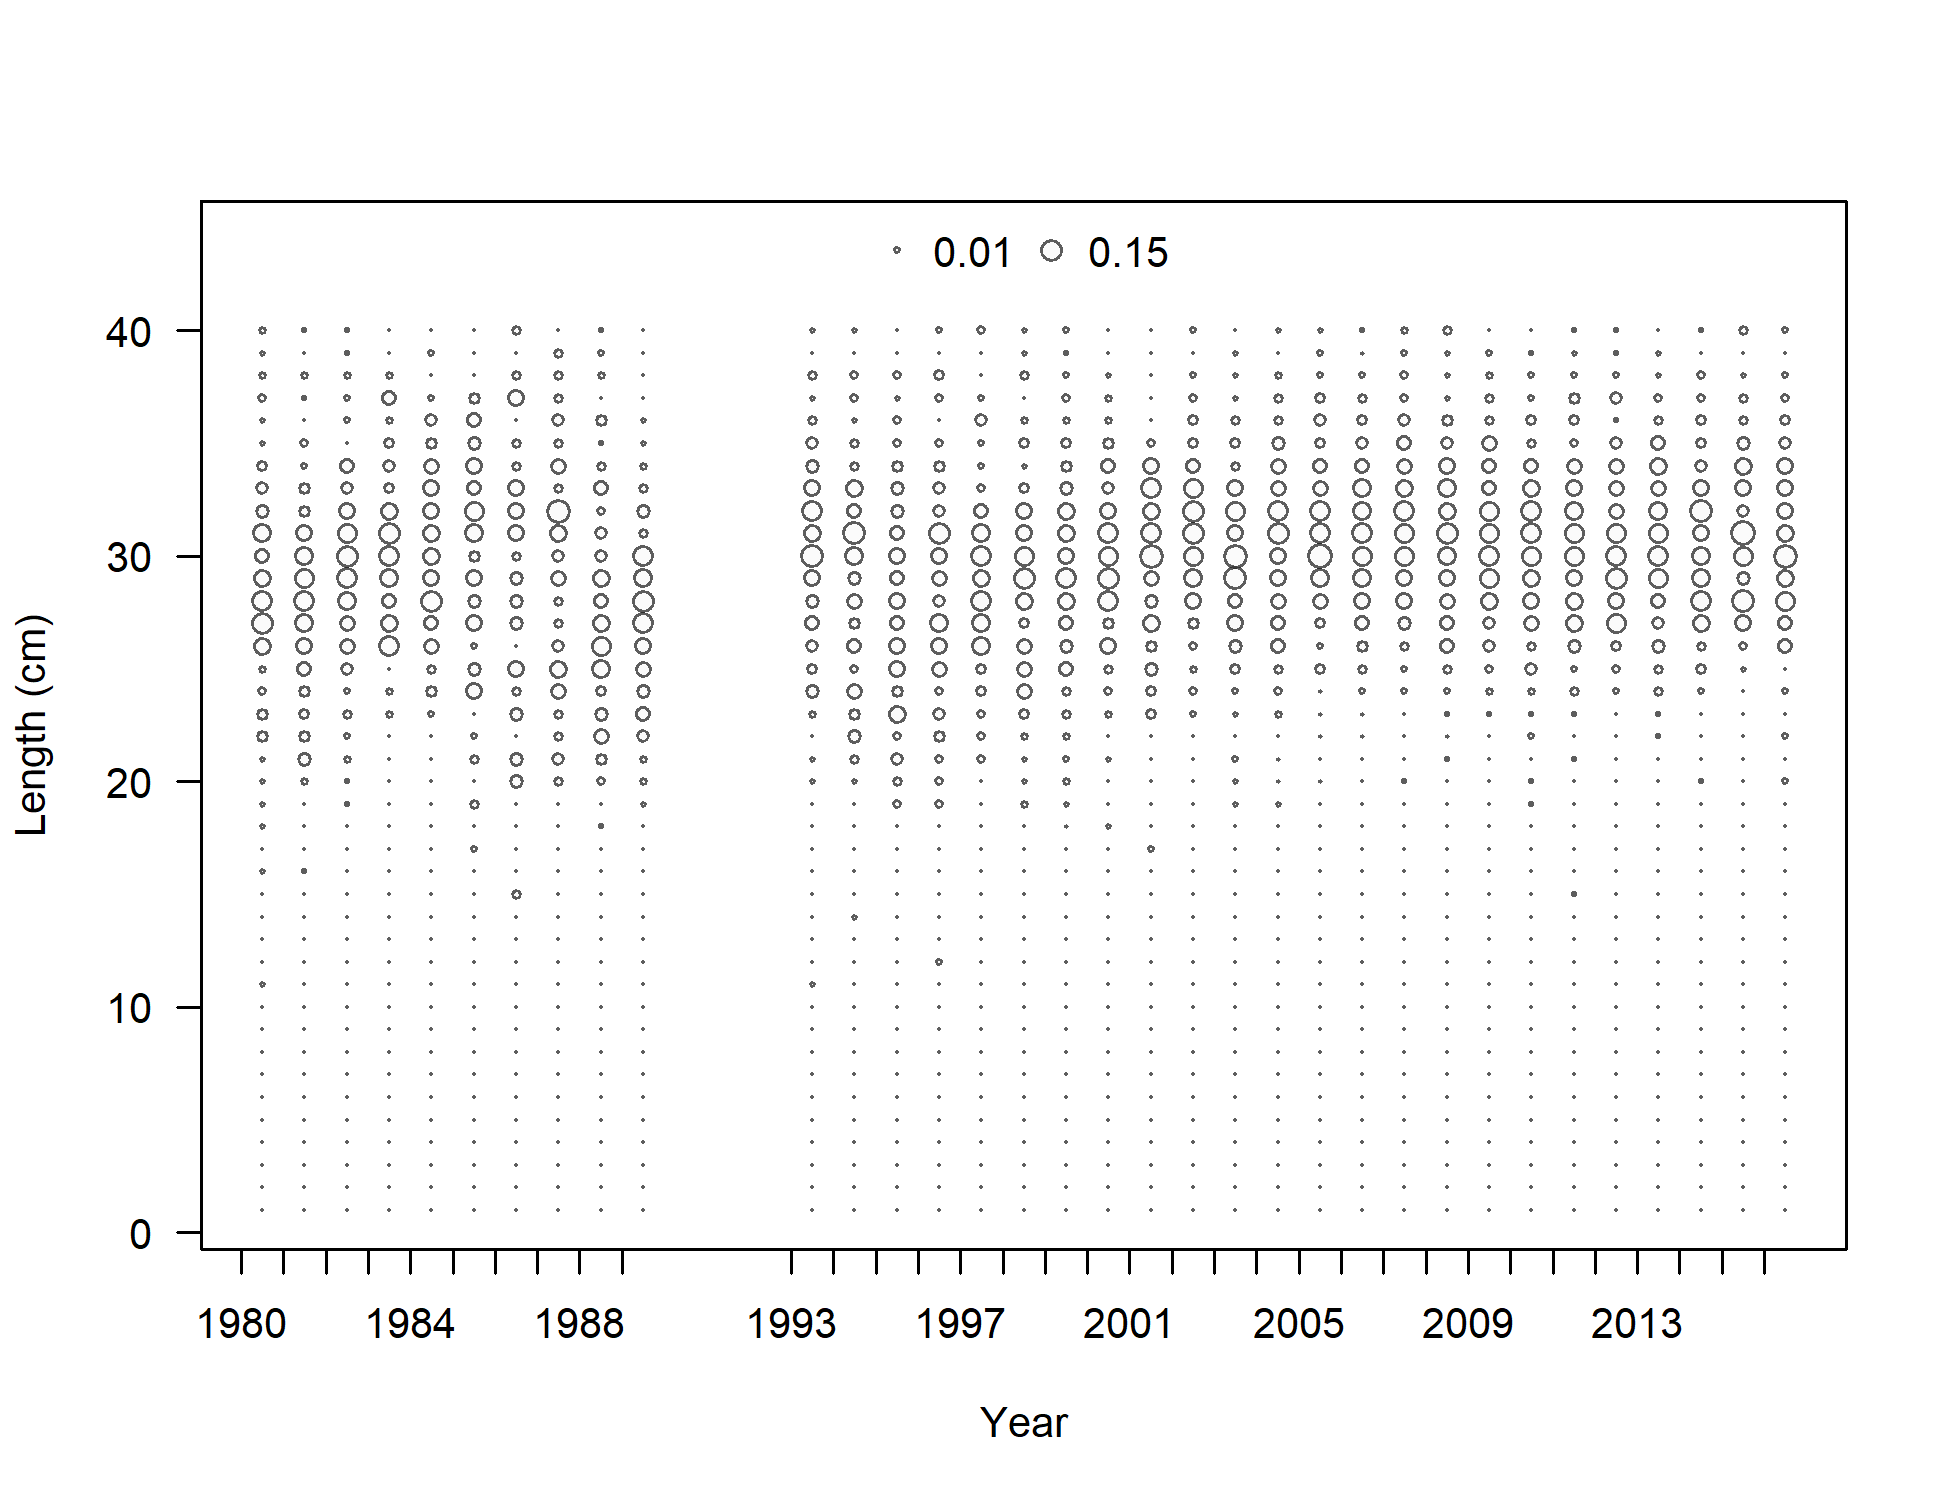
\includegraphics[height=3cm]{r4ss/plots_mod1/comp_lendat_bubflt4mkt2.png}

Recreational party/charter fleet
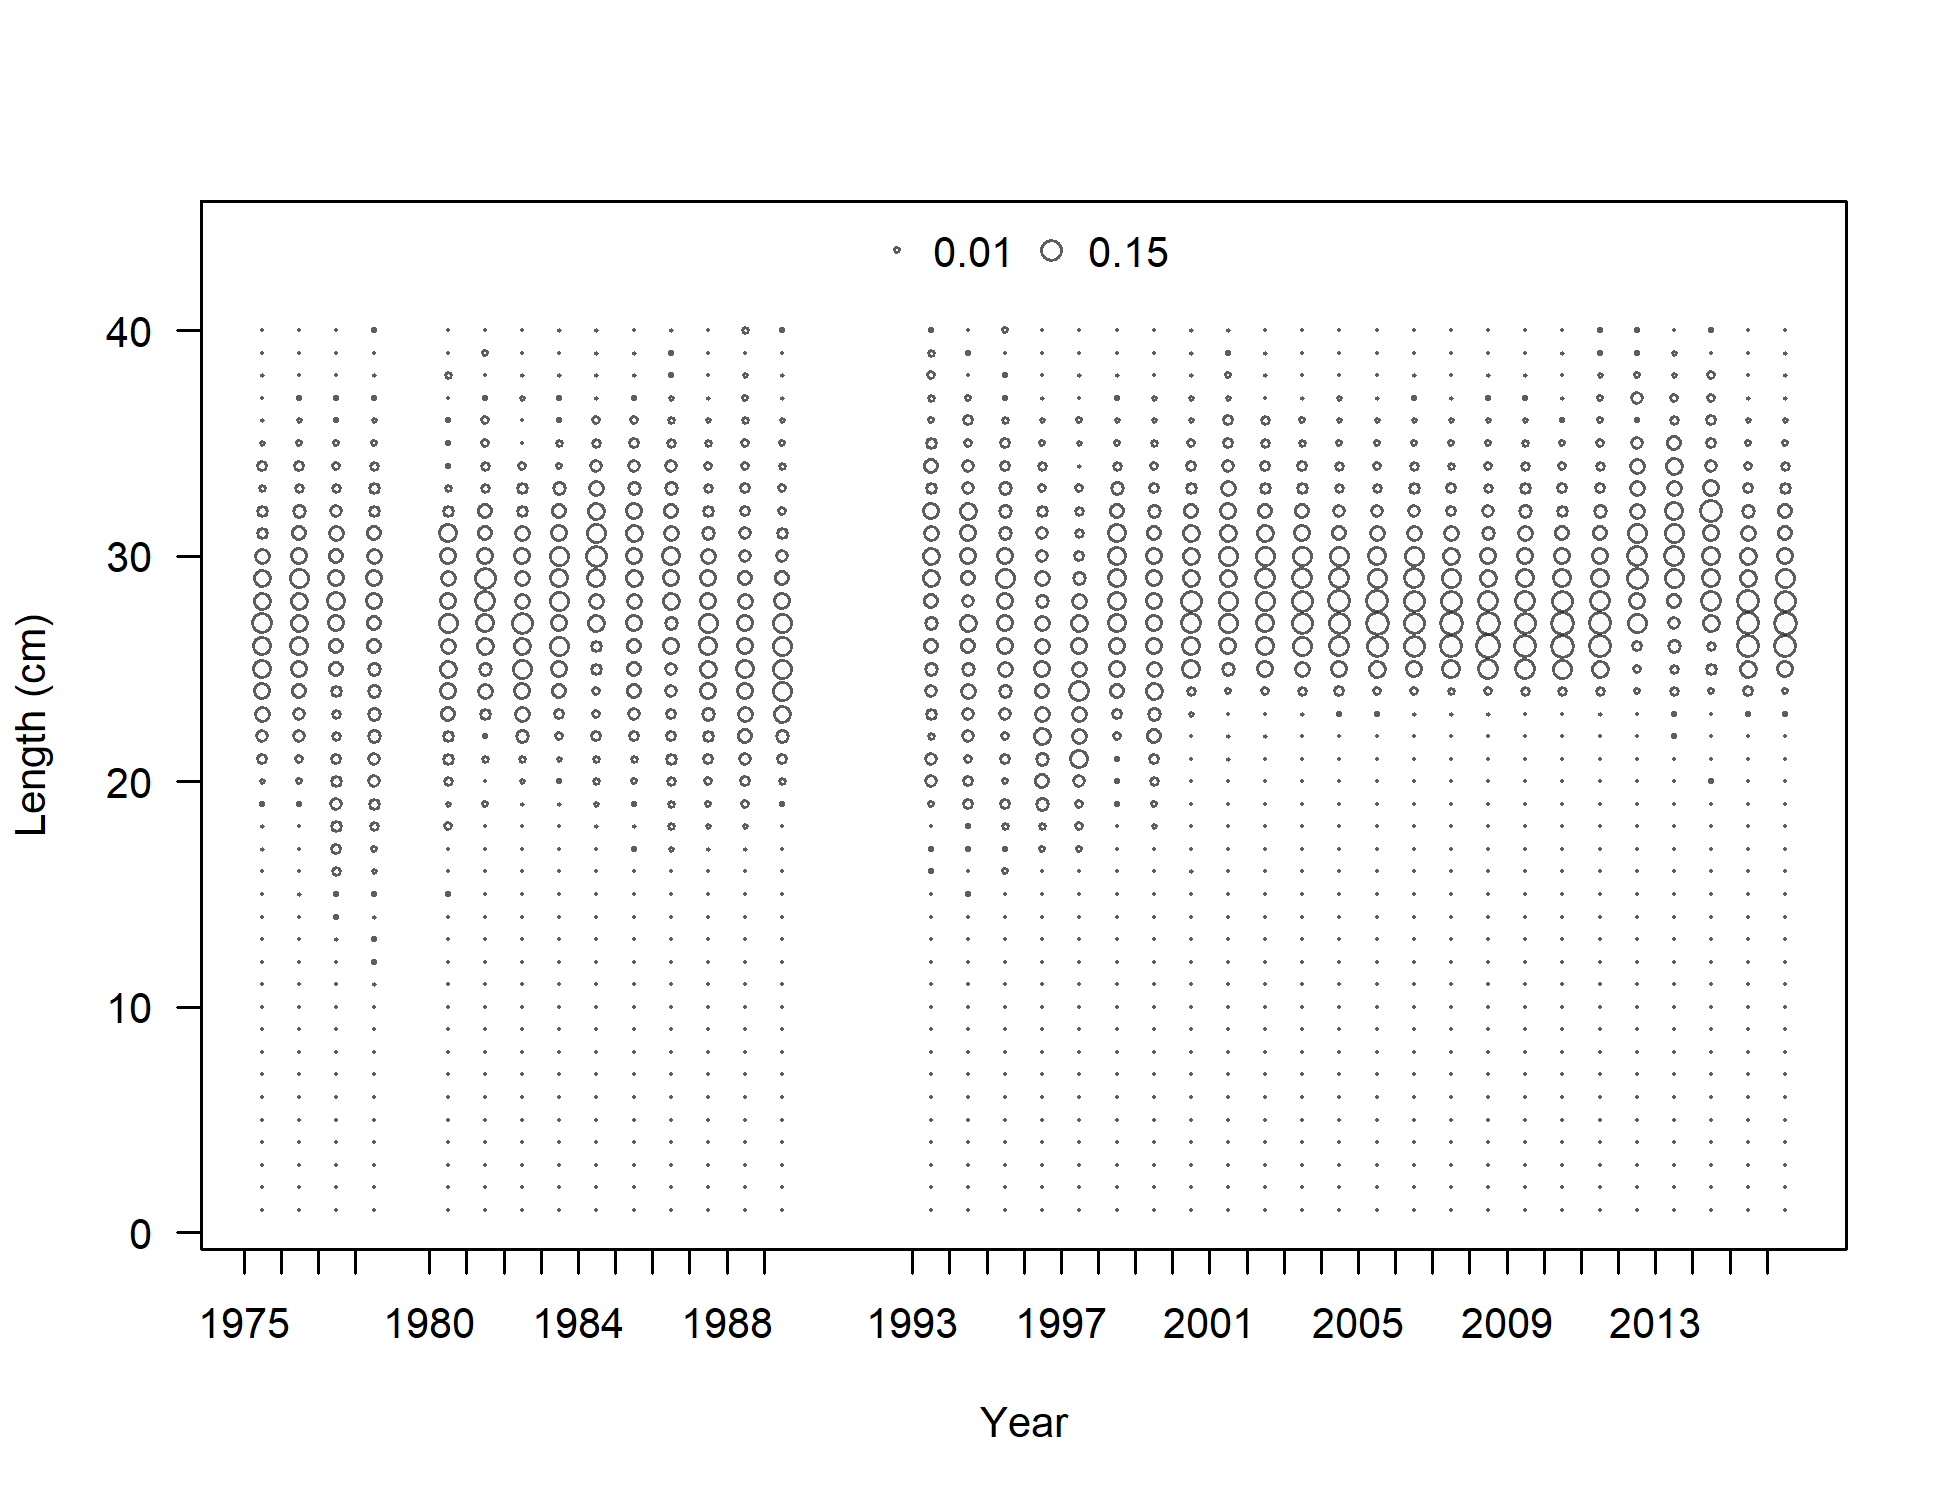
\includegraphics[height=3cm]{r4ss/plots_mod1/comp_lendat_bubflt5mkt2_page2.png}
\endcol
 \begincol{.5\textwidth} \centering

Recreational dead discards
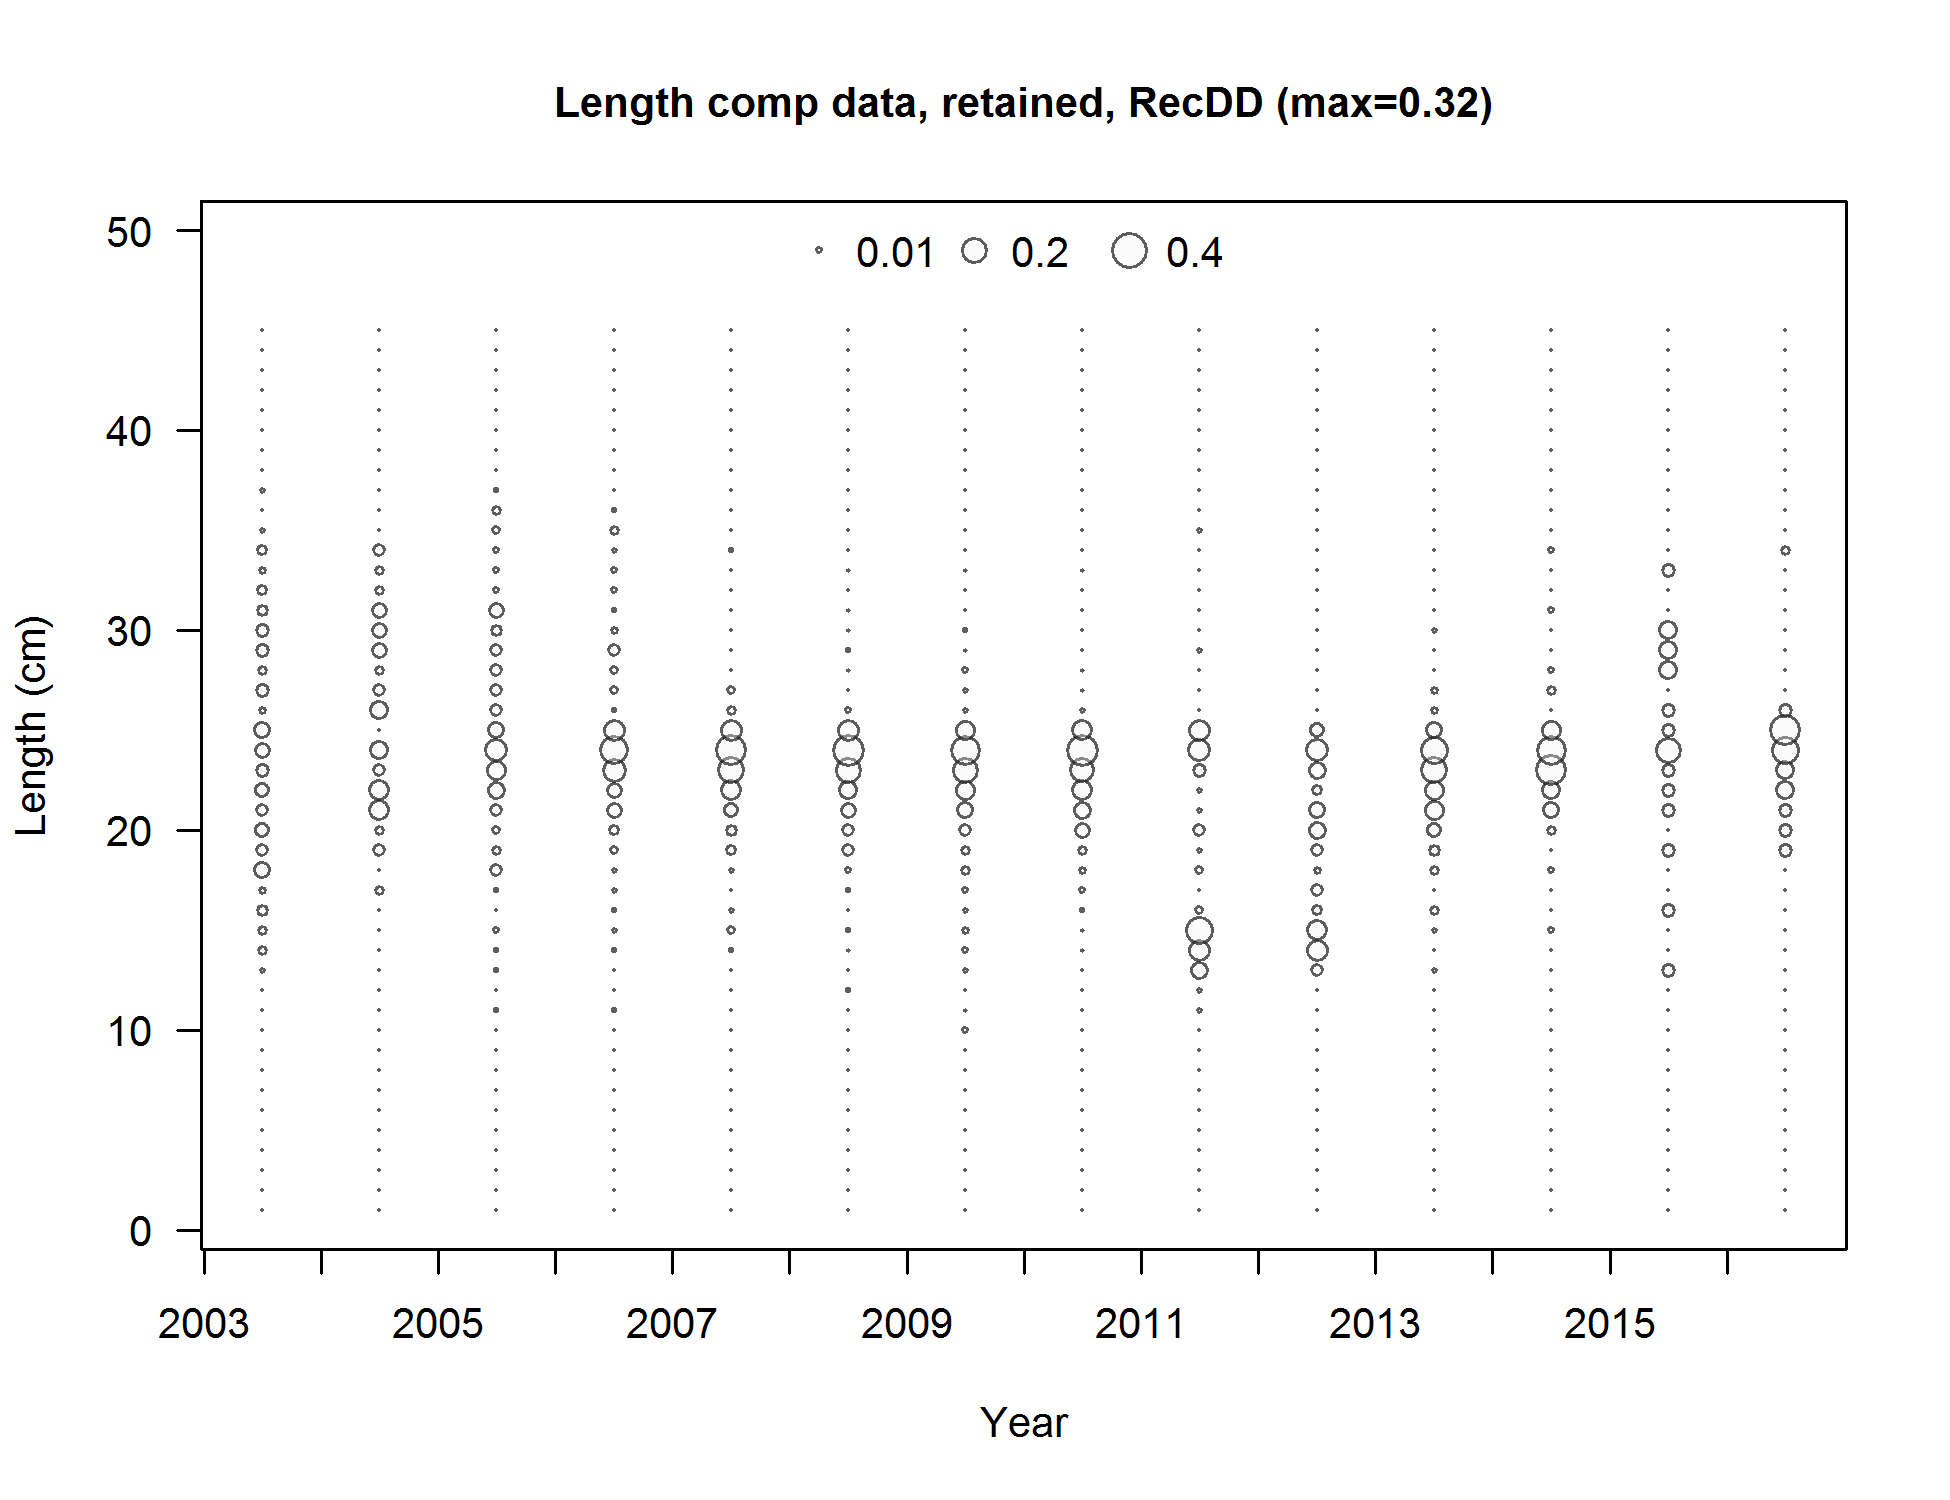
\includegraphics[height=4cm]{r4ss/plots_mod1/comp_lendat_bubflt6mkt2.png}
\endcol
\endcols

\end{frame}

\begin{frame}{Research Length Composition}

\begincols
 \begincol{.5\textwidth} POTW survey
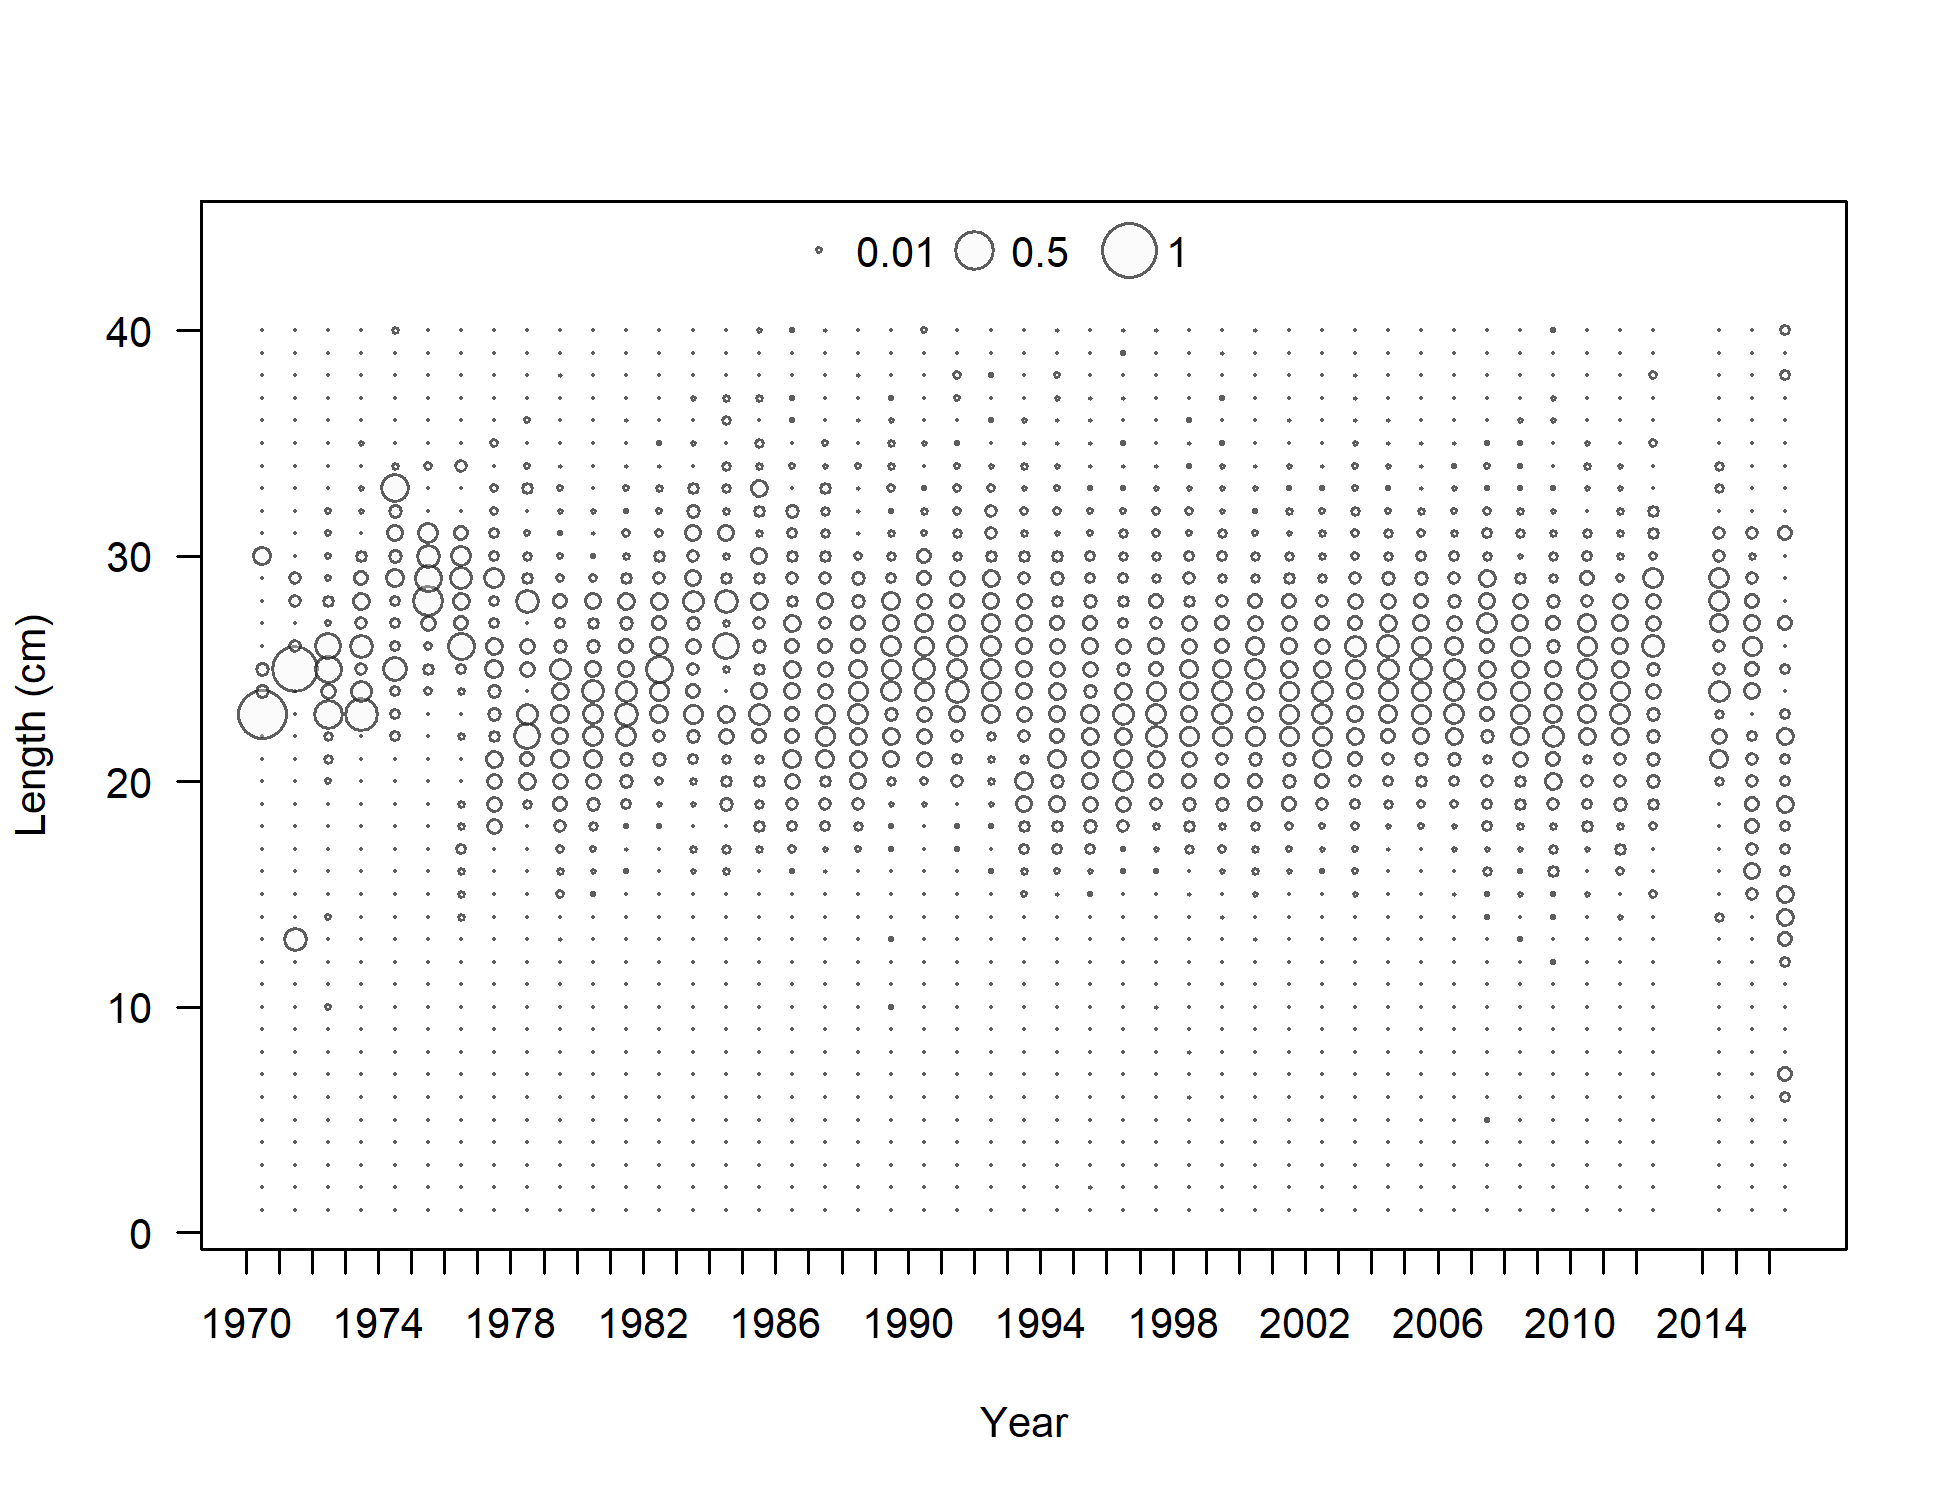
\includegraphics[height=3cm]{r4ss/plots_mod1/comp_lendat_bubflt7mkt2_page2.png}

Impingement survey
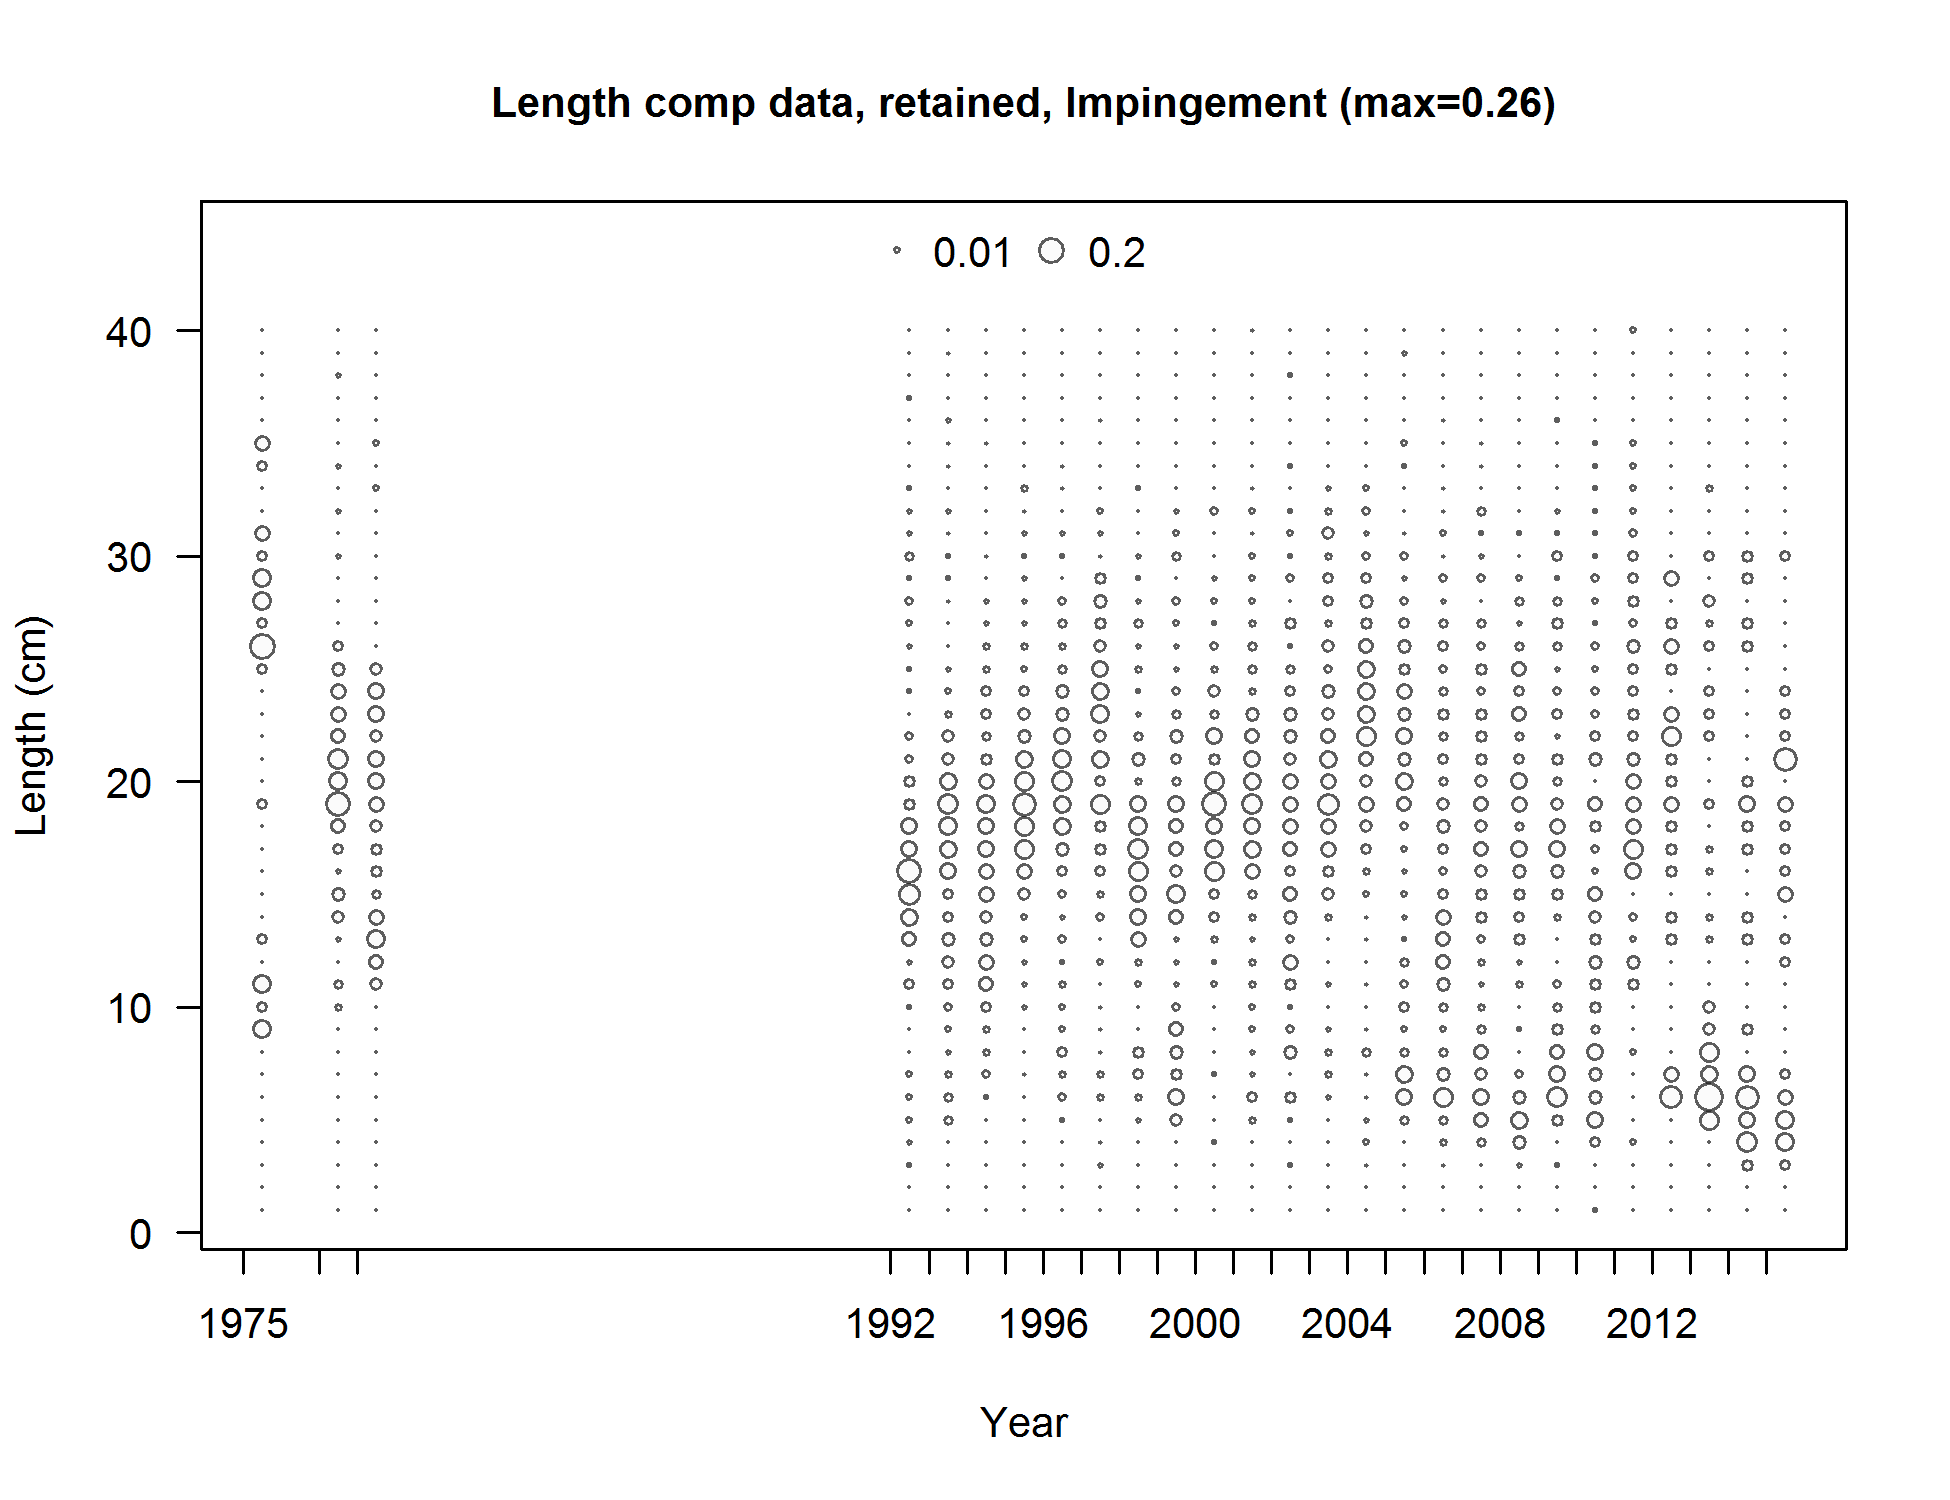
\includegraphics[height=3cm]{r4ss/plots_mod1/comp_lendat_bubflt10mkt2.png}

Bight trawl survey
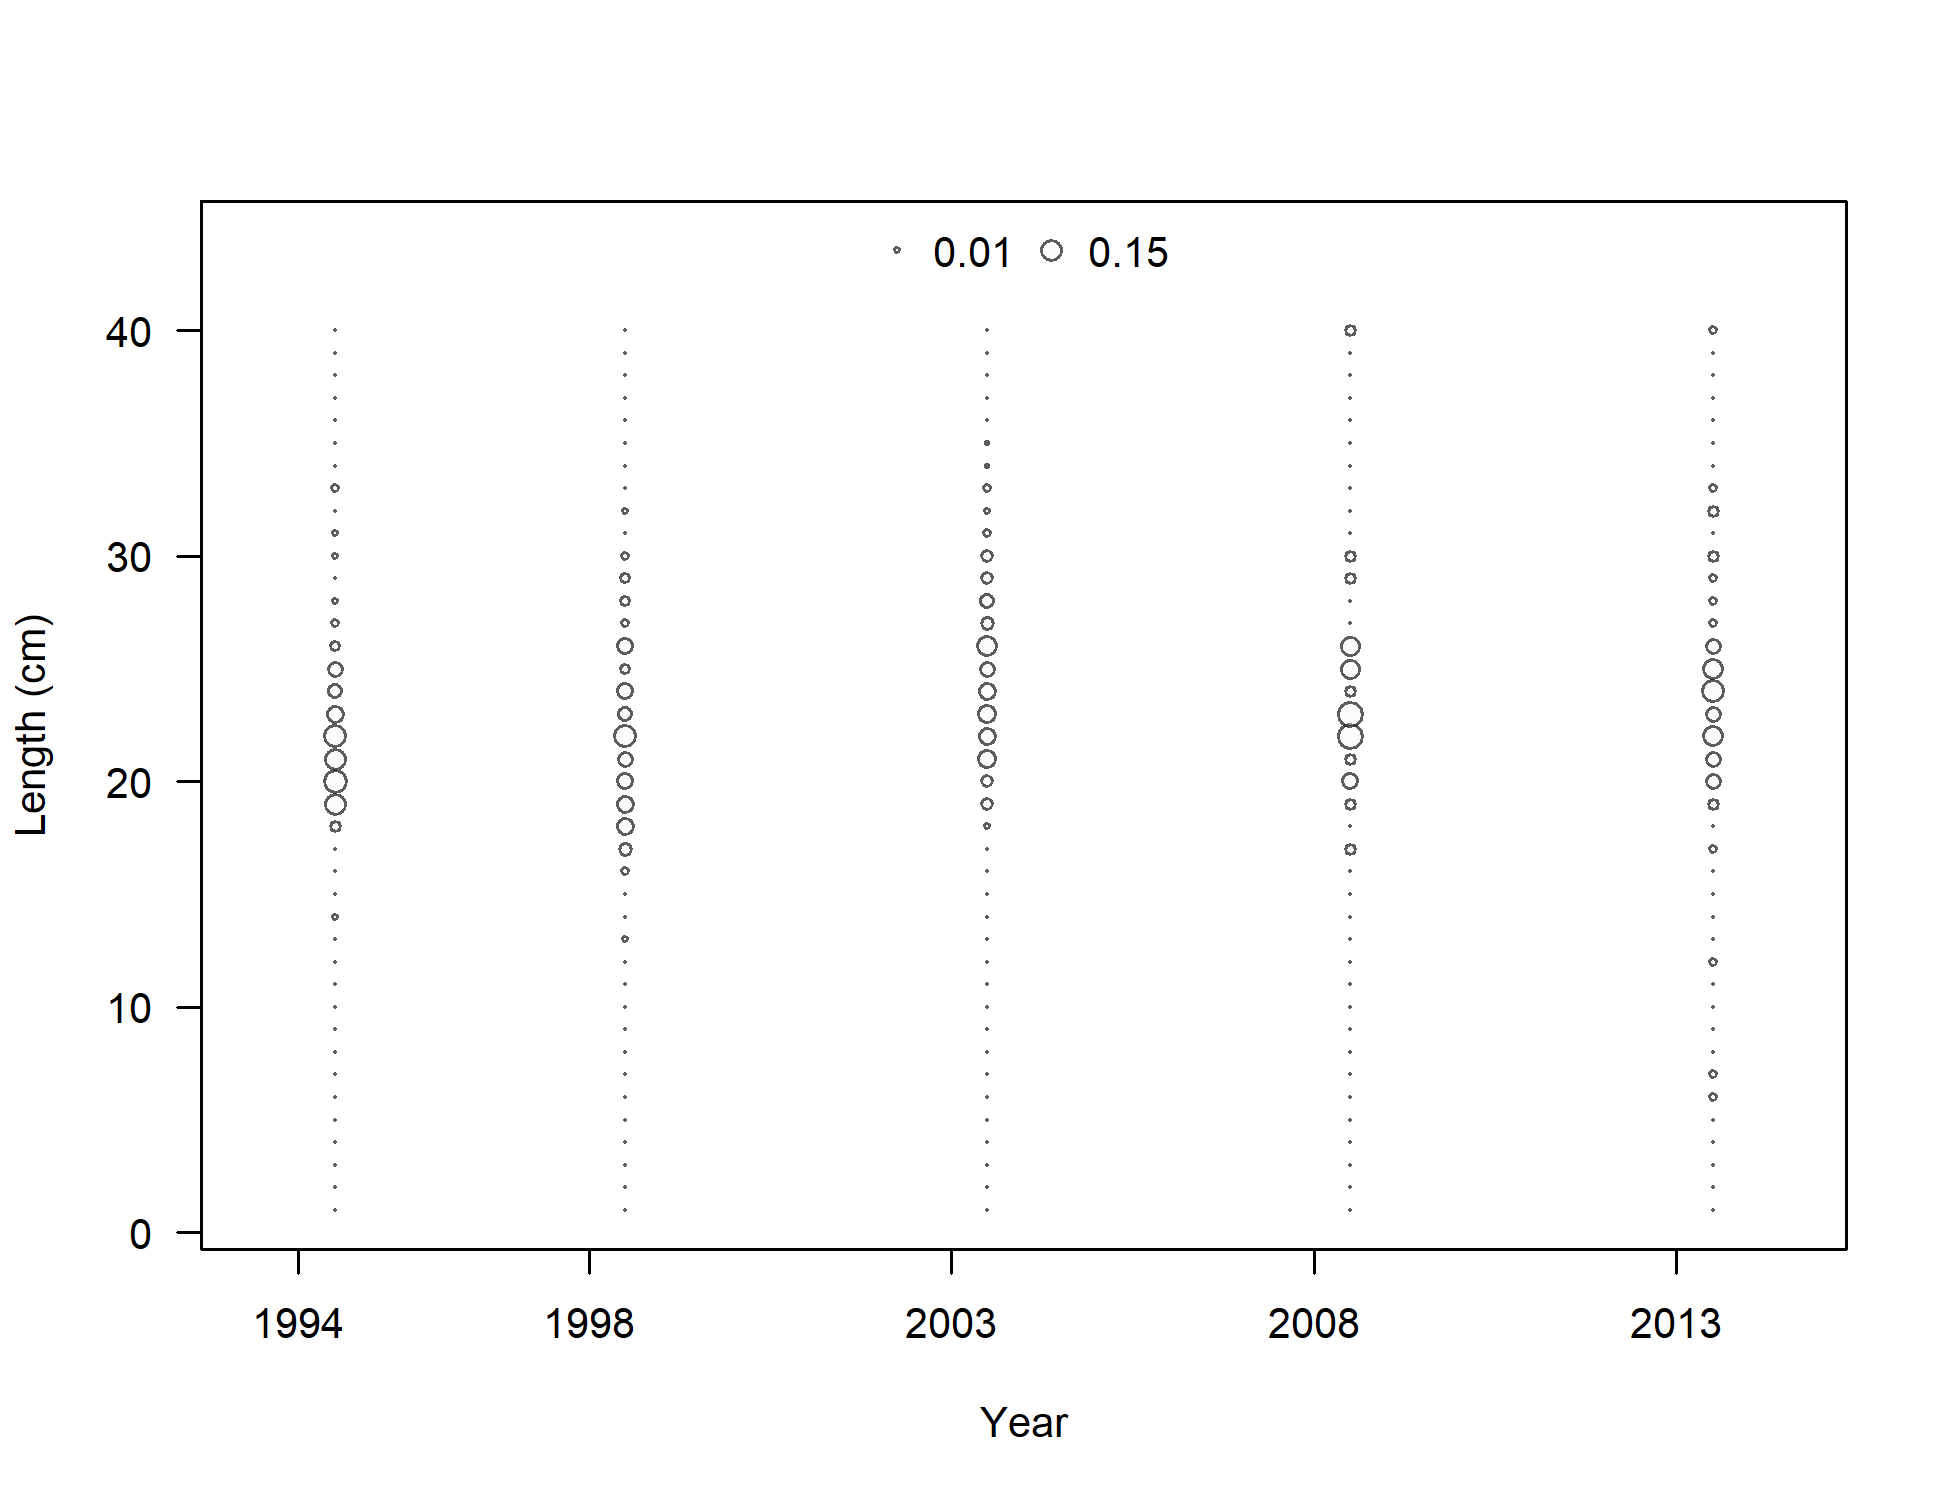
\includegraphics[height=3cm]{r4ss/plots_mod1/comp_lendat_bubflt11mkt2.png}
\endcol
\endcols

\end{frame}

\begin{frame}{NWFSC Length and Age Composition}

Note: females in red and males in blue \begincols
 \begincol{.5\textwidth}
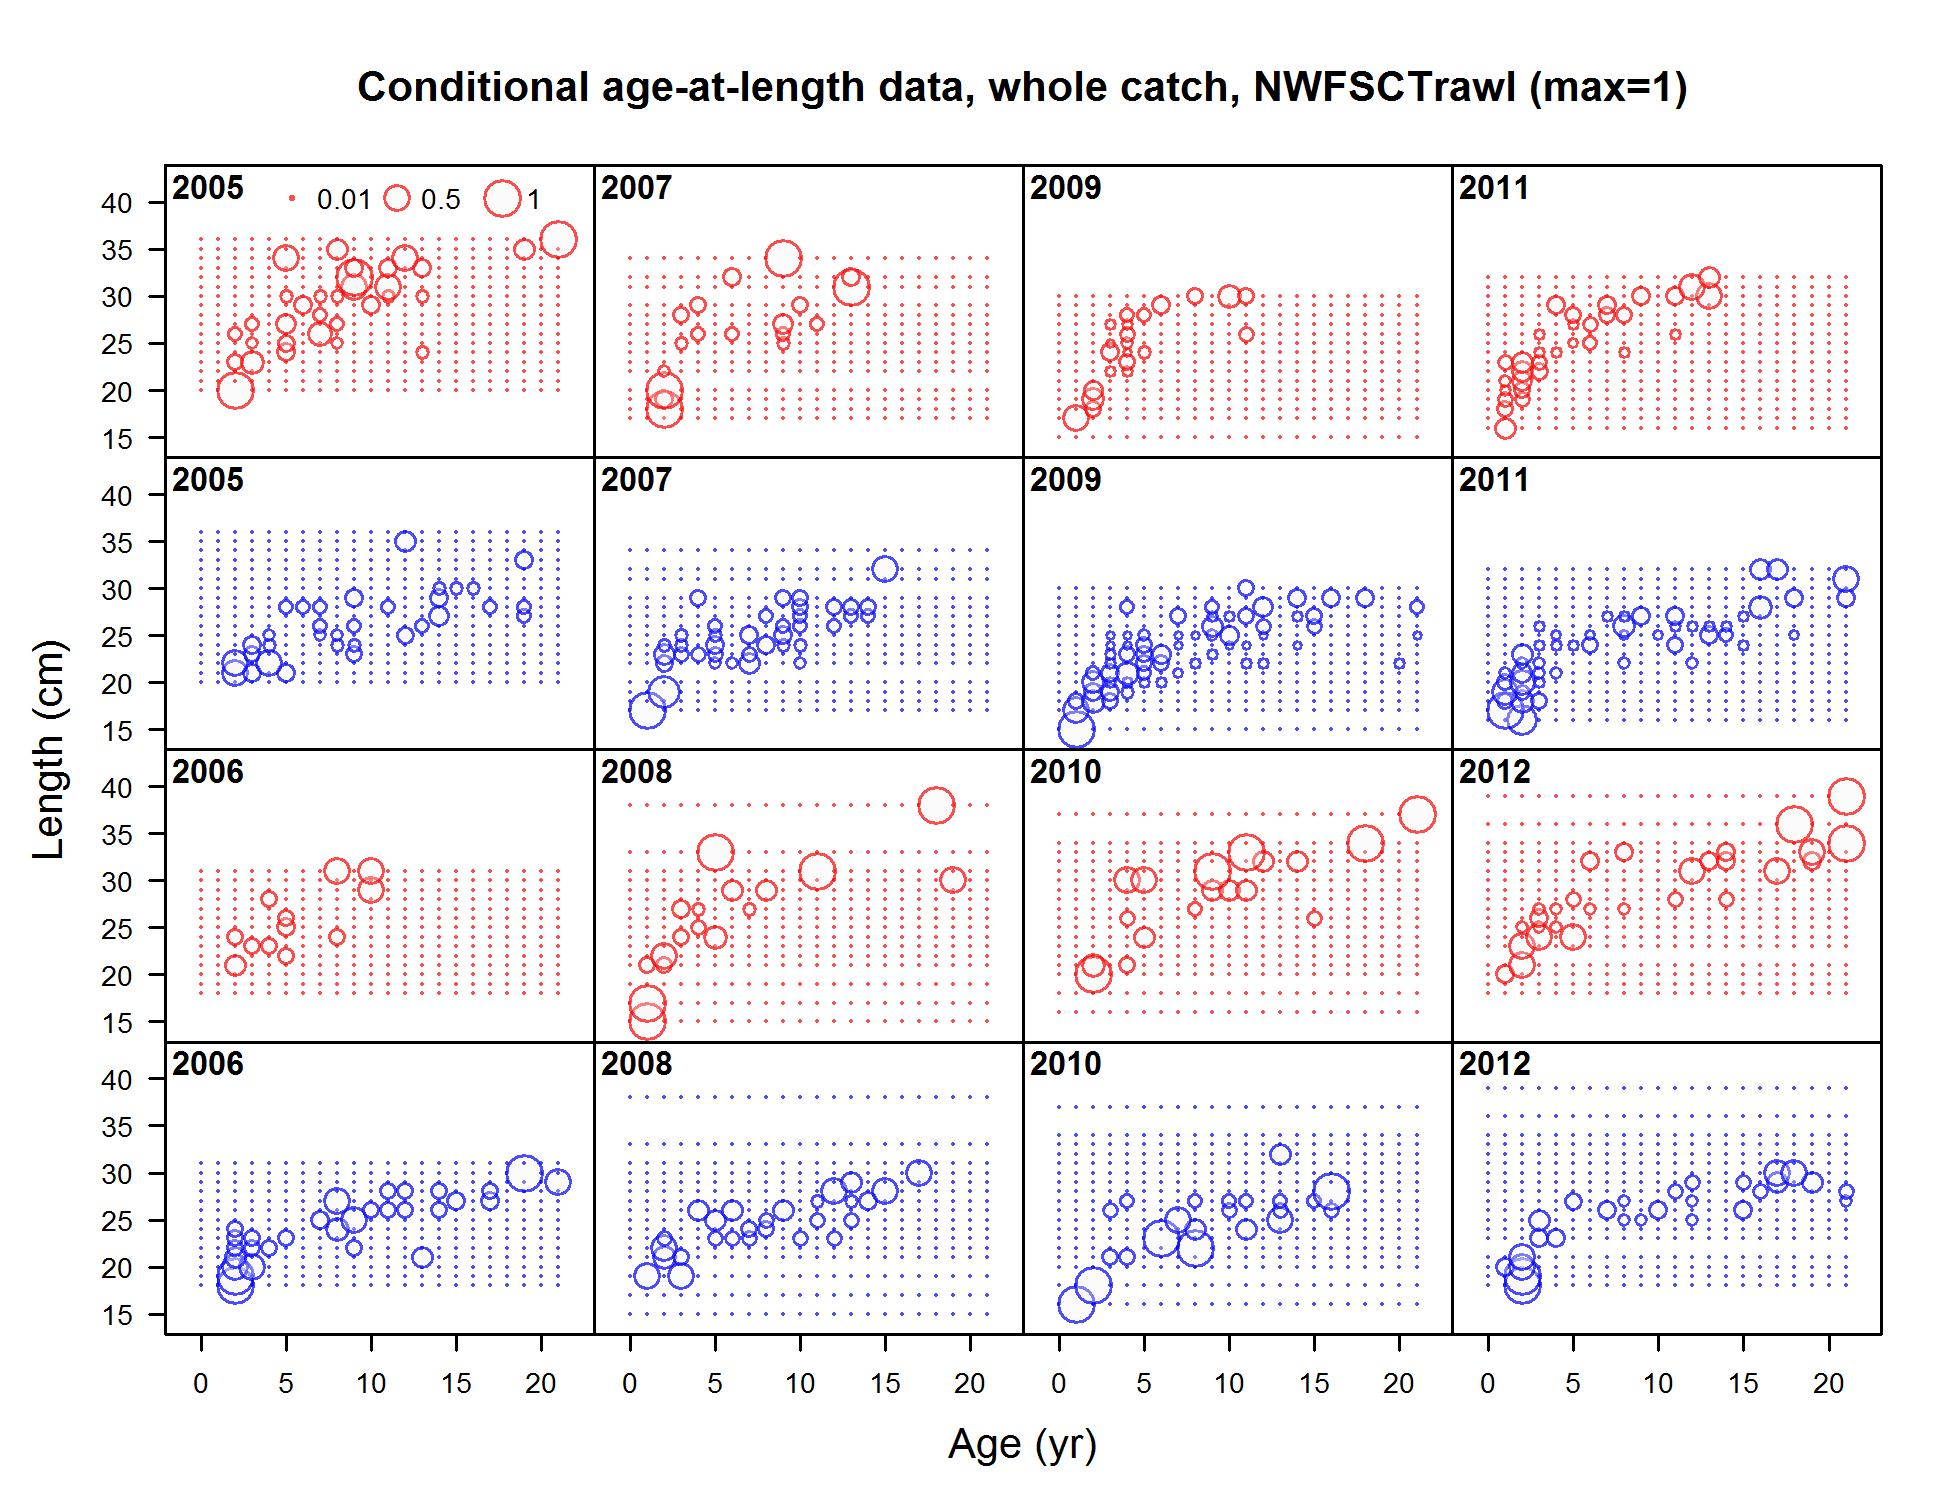
\includegraphics[height=.5\textheight]{r4ss/plots_mod1/comp_condAALdat_bubflt8mkt0_page1.png}
\endcol
 \begincol{.5\textwidth}
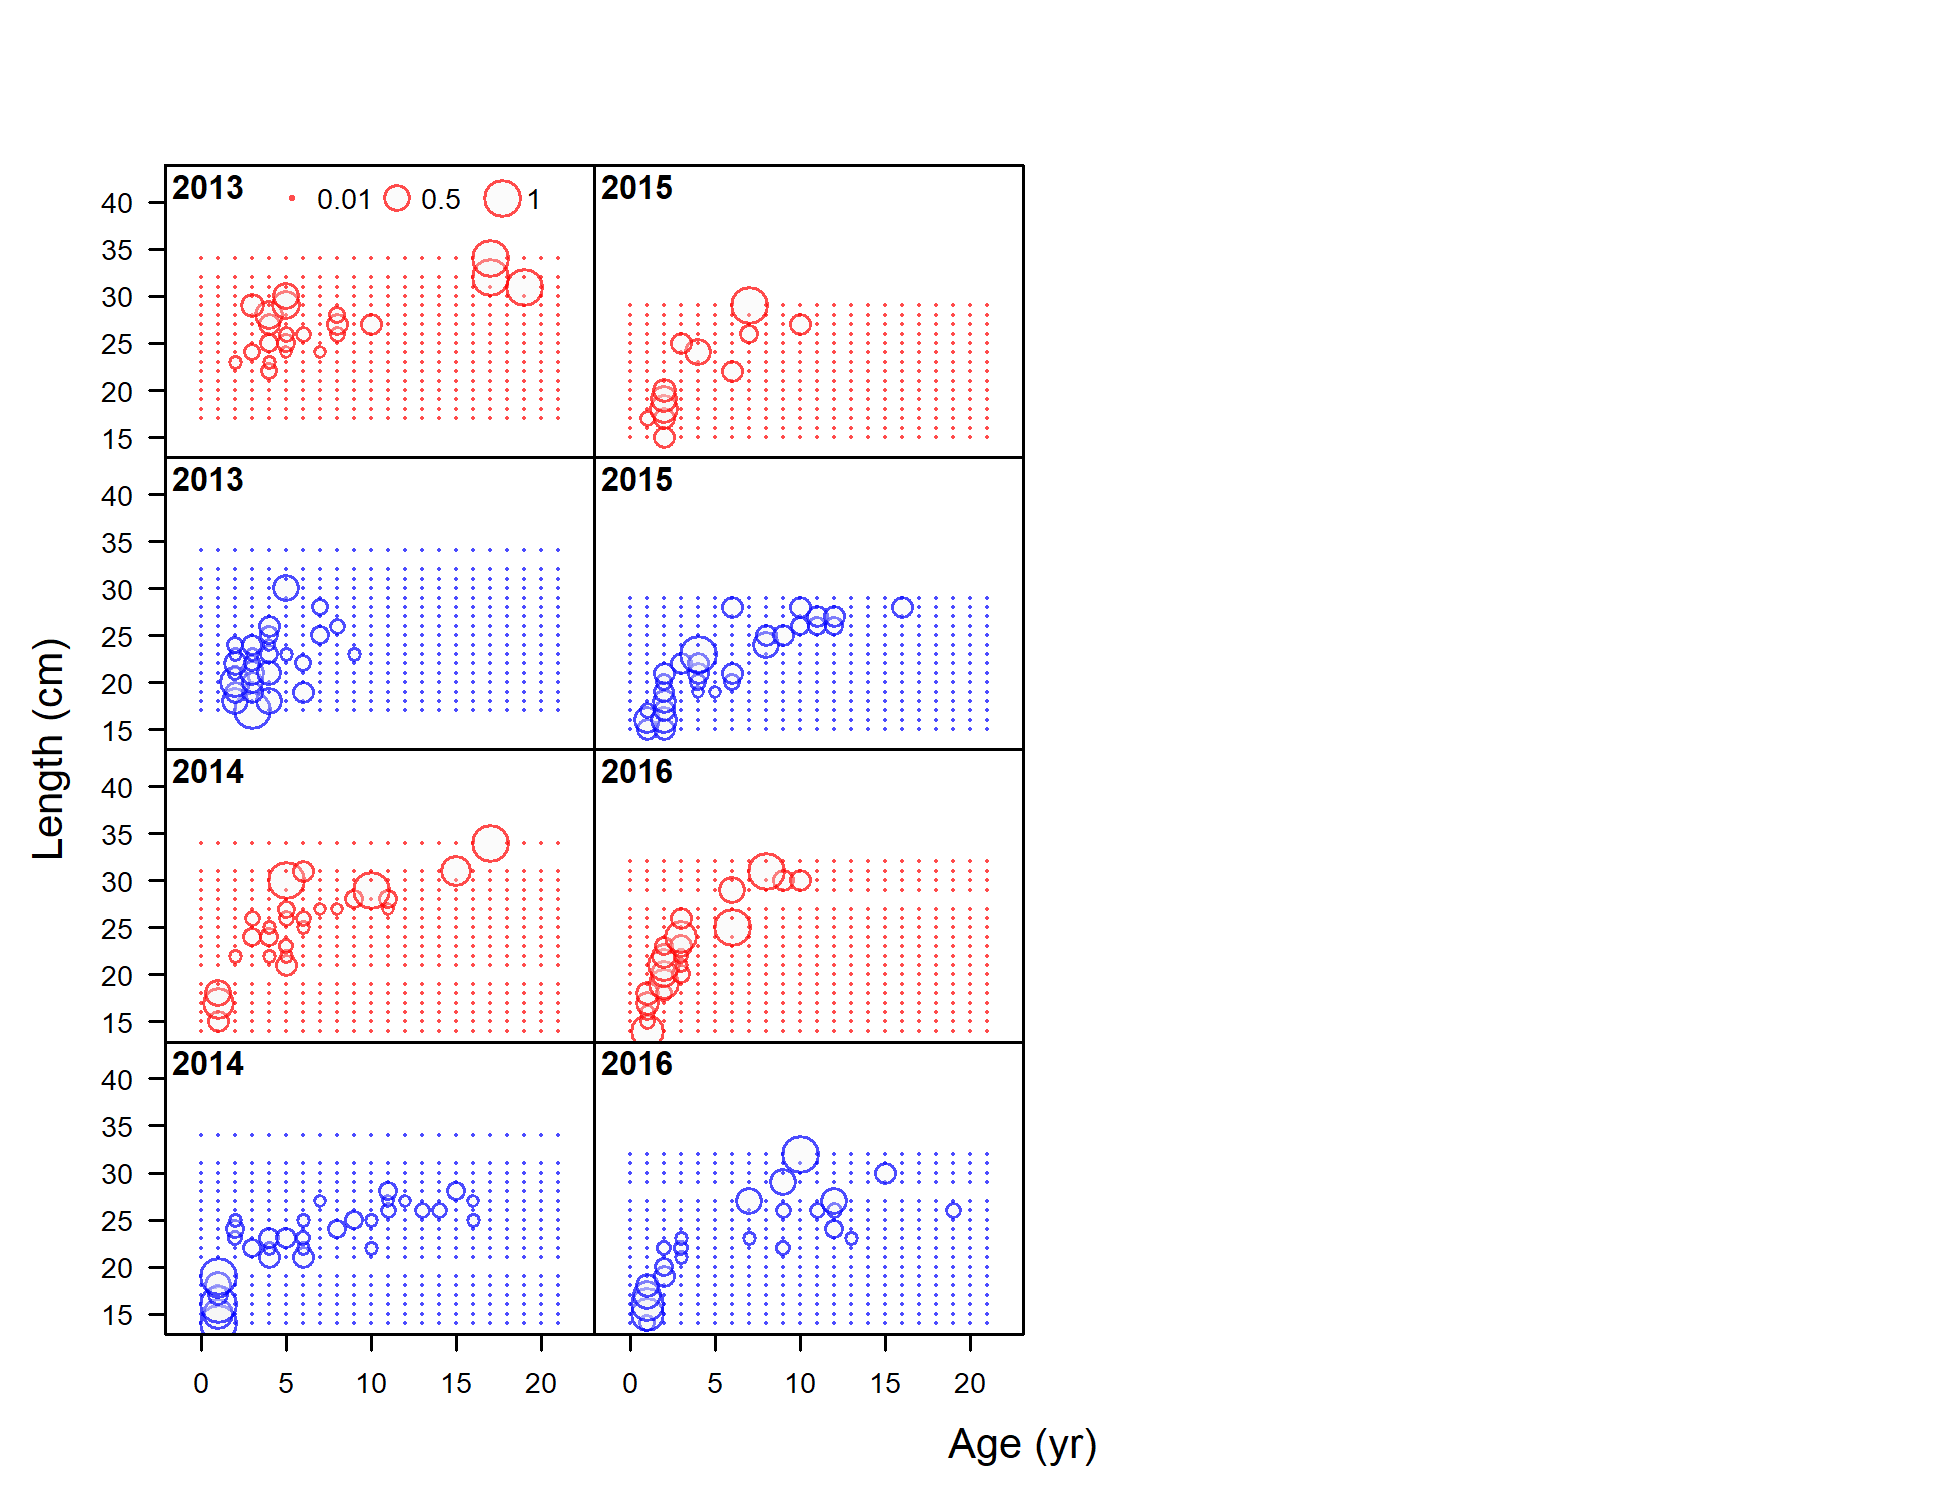
\includegraphics[height=.5\textheight]{r4ss/plots_mod1/comp_condAALdat_bubflt8mkt0_page2.png}
\endcol
\endcols

\end{frame}

\section{Biological}\label{biological}

\begin{frame}{Length data}

\begin{itemize}
\item[$\bullet$] 2005 assessment used standard length
\item[$\bullet$] Impingement, POTW, and Bight surveys measure standard length
\item[$\bullet$] 2017 assessment uses total length (conversion based on a CDFW halibut trawl study; measured both SL and TL)
\item[$\bullet$] To avoid gaps in TL length bins, TL = SL - 0.5 + U[0,1] 
\end{itemize}

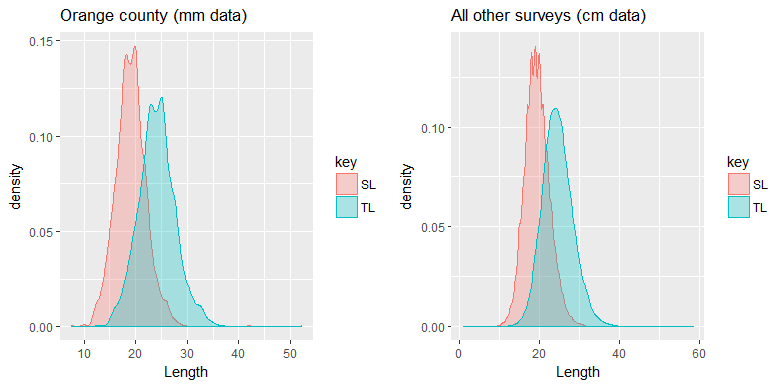
\includegraphics[height=.5\textheight]{Figures/SL_to_TL_compare.png}

\end{frame}

\begin{frame}{Length data}

POTW lengths \begincols
 \begincol{.4\textwidth}
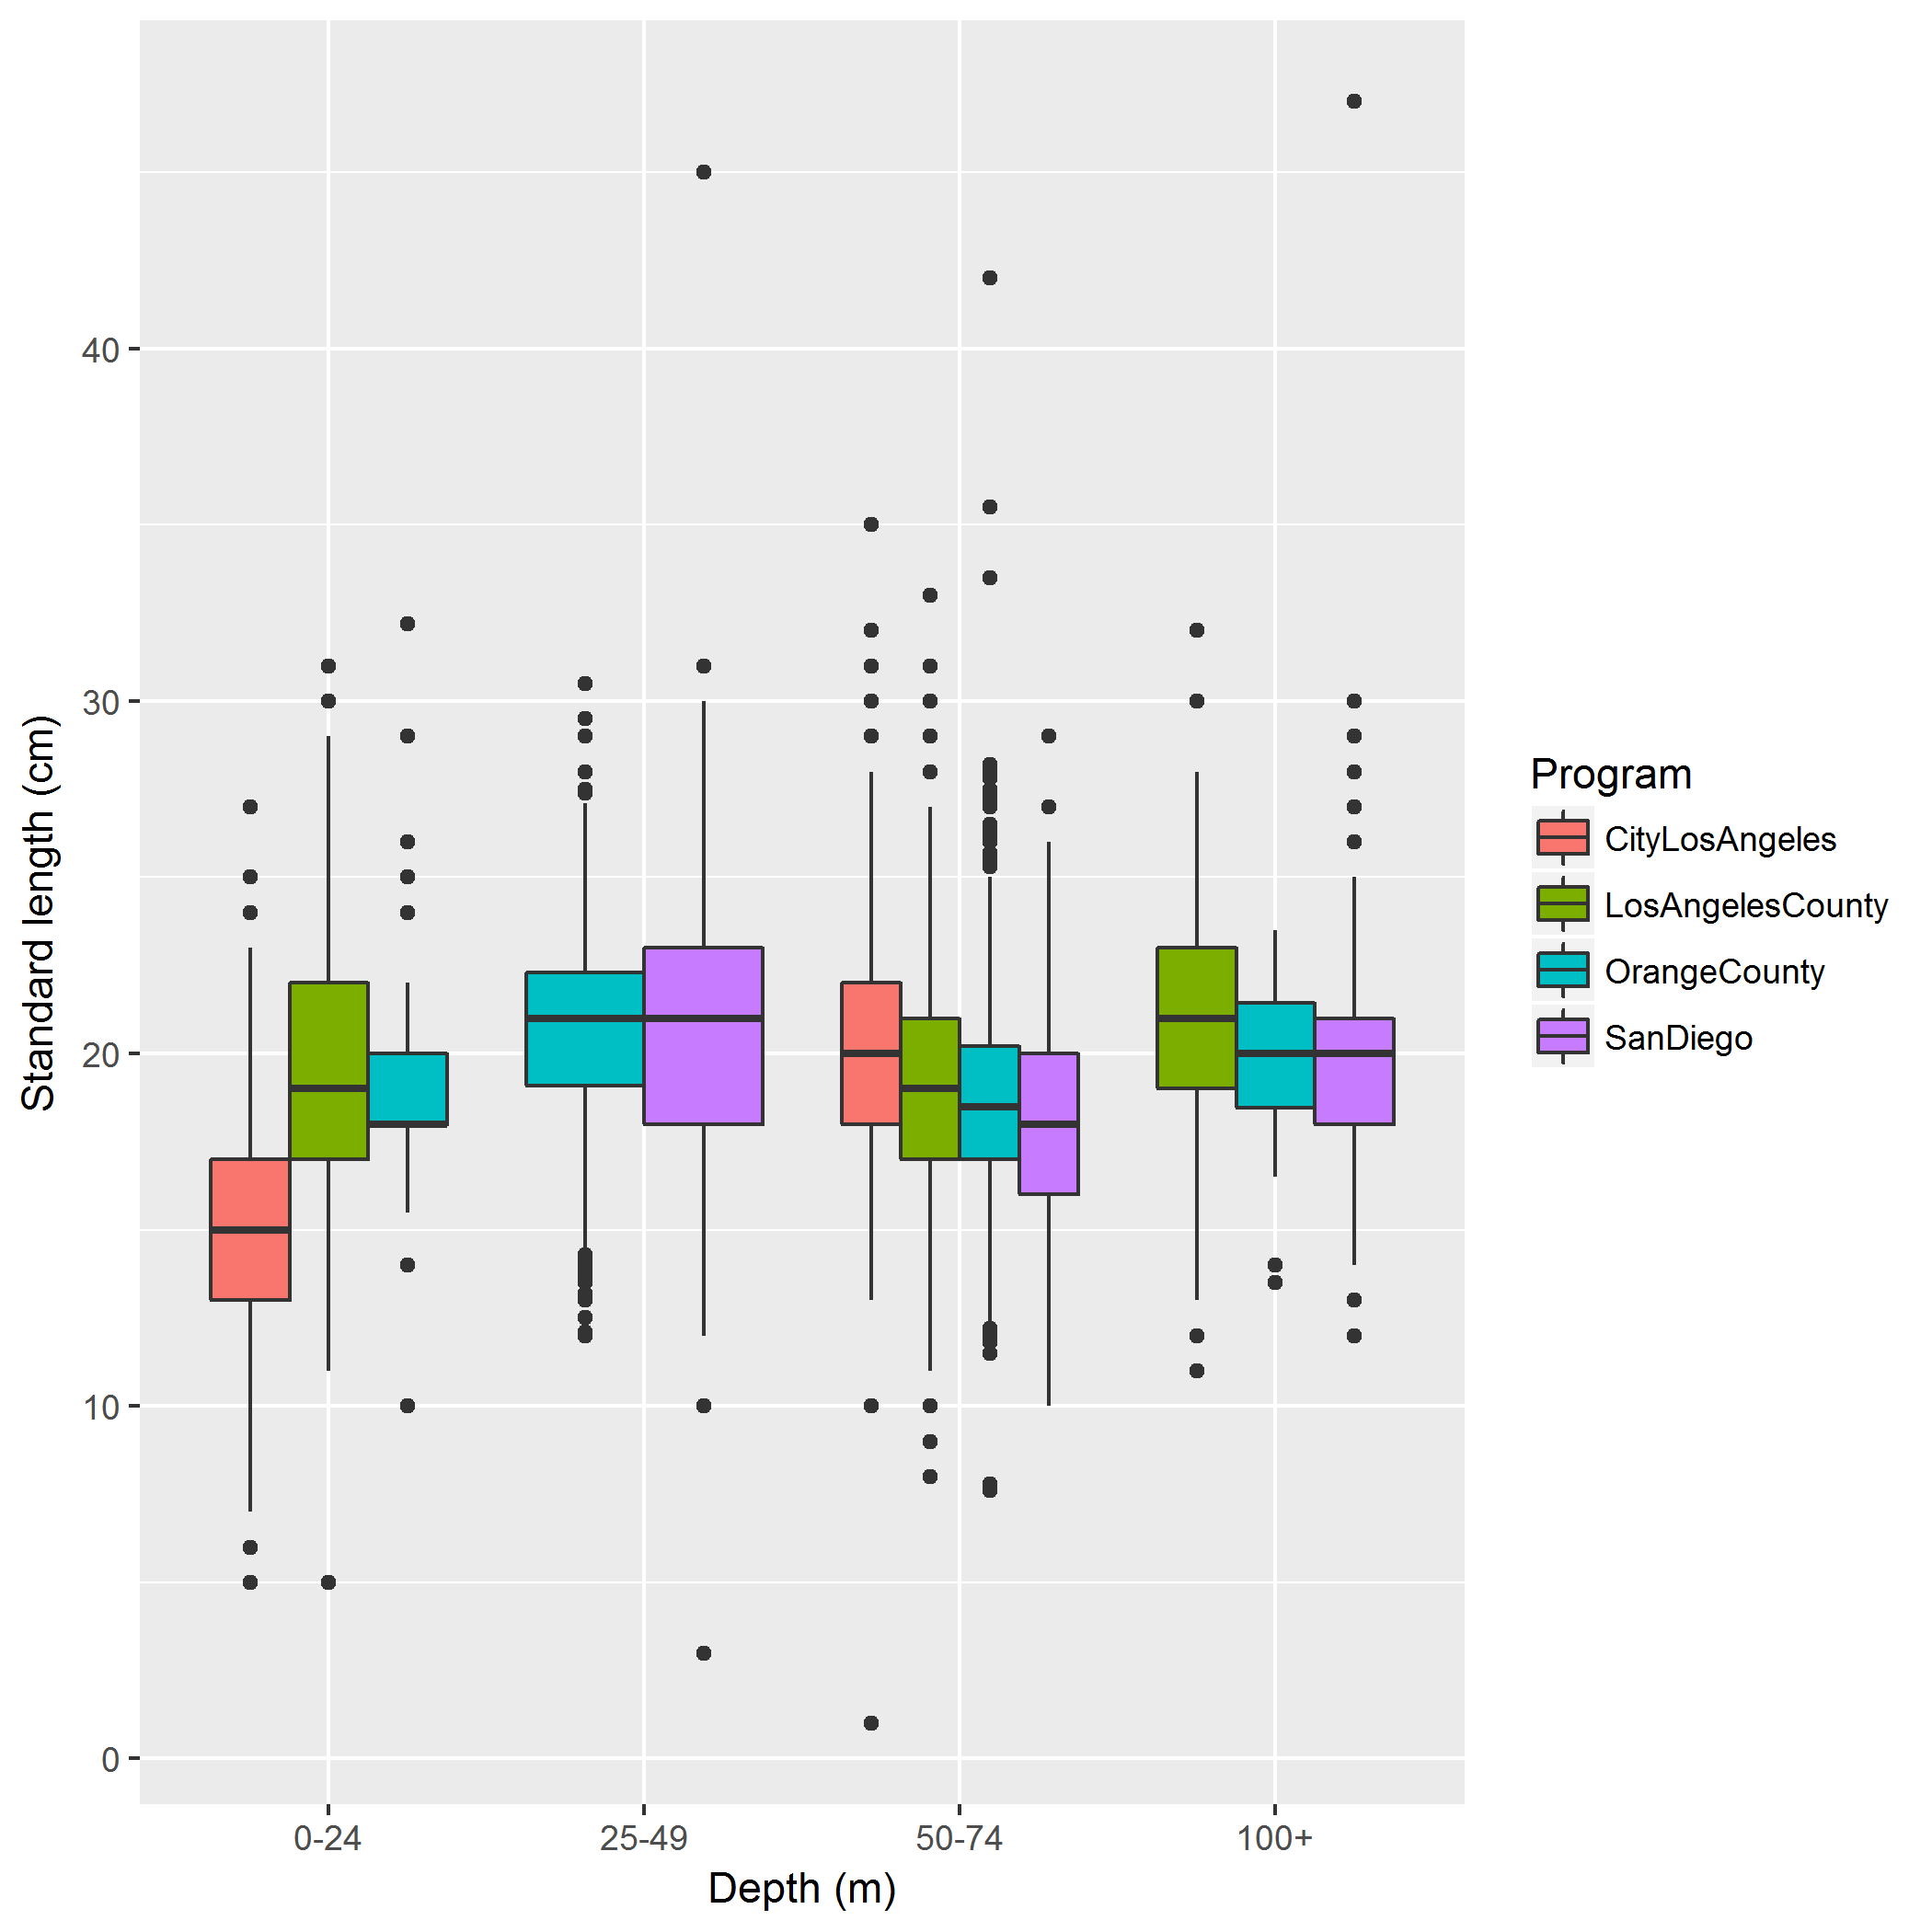
\includegraphics{Figures/Fleet7_Sanitation_lengthboxplots.png} \endcol
 \begincol{.6\textwidth}
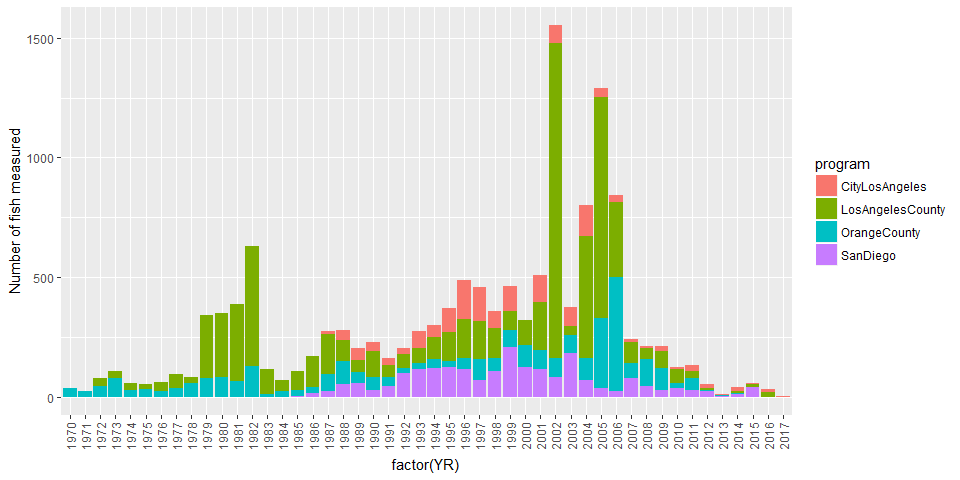
\includegraphics{Figures/Fleet7_Sanitation_length_source.png}\\
\endcol
\endcols

\end{frame}

\begin{frame}{Length-at-Age}

\begincols
 \begincol{.4\textwidth}
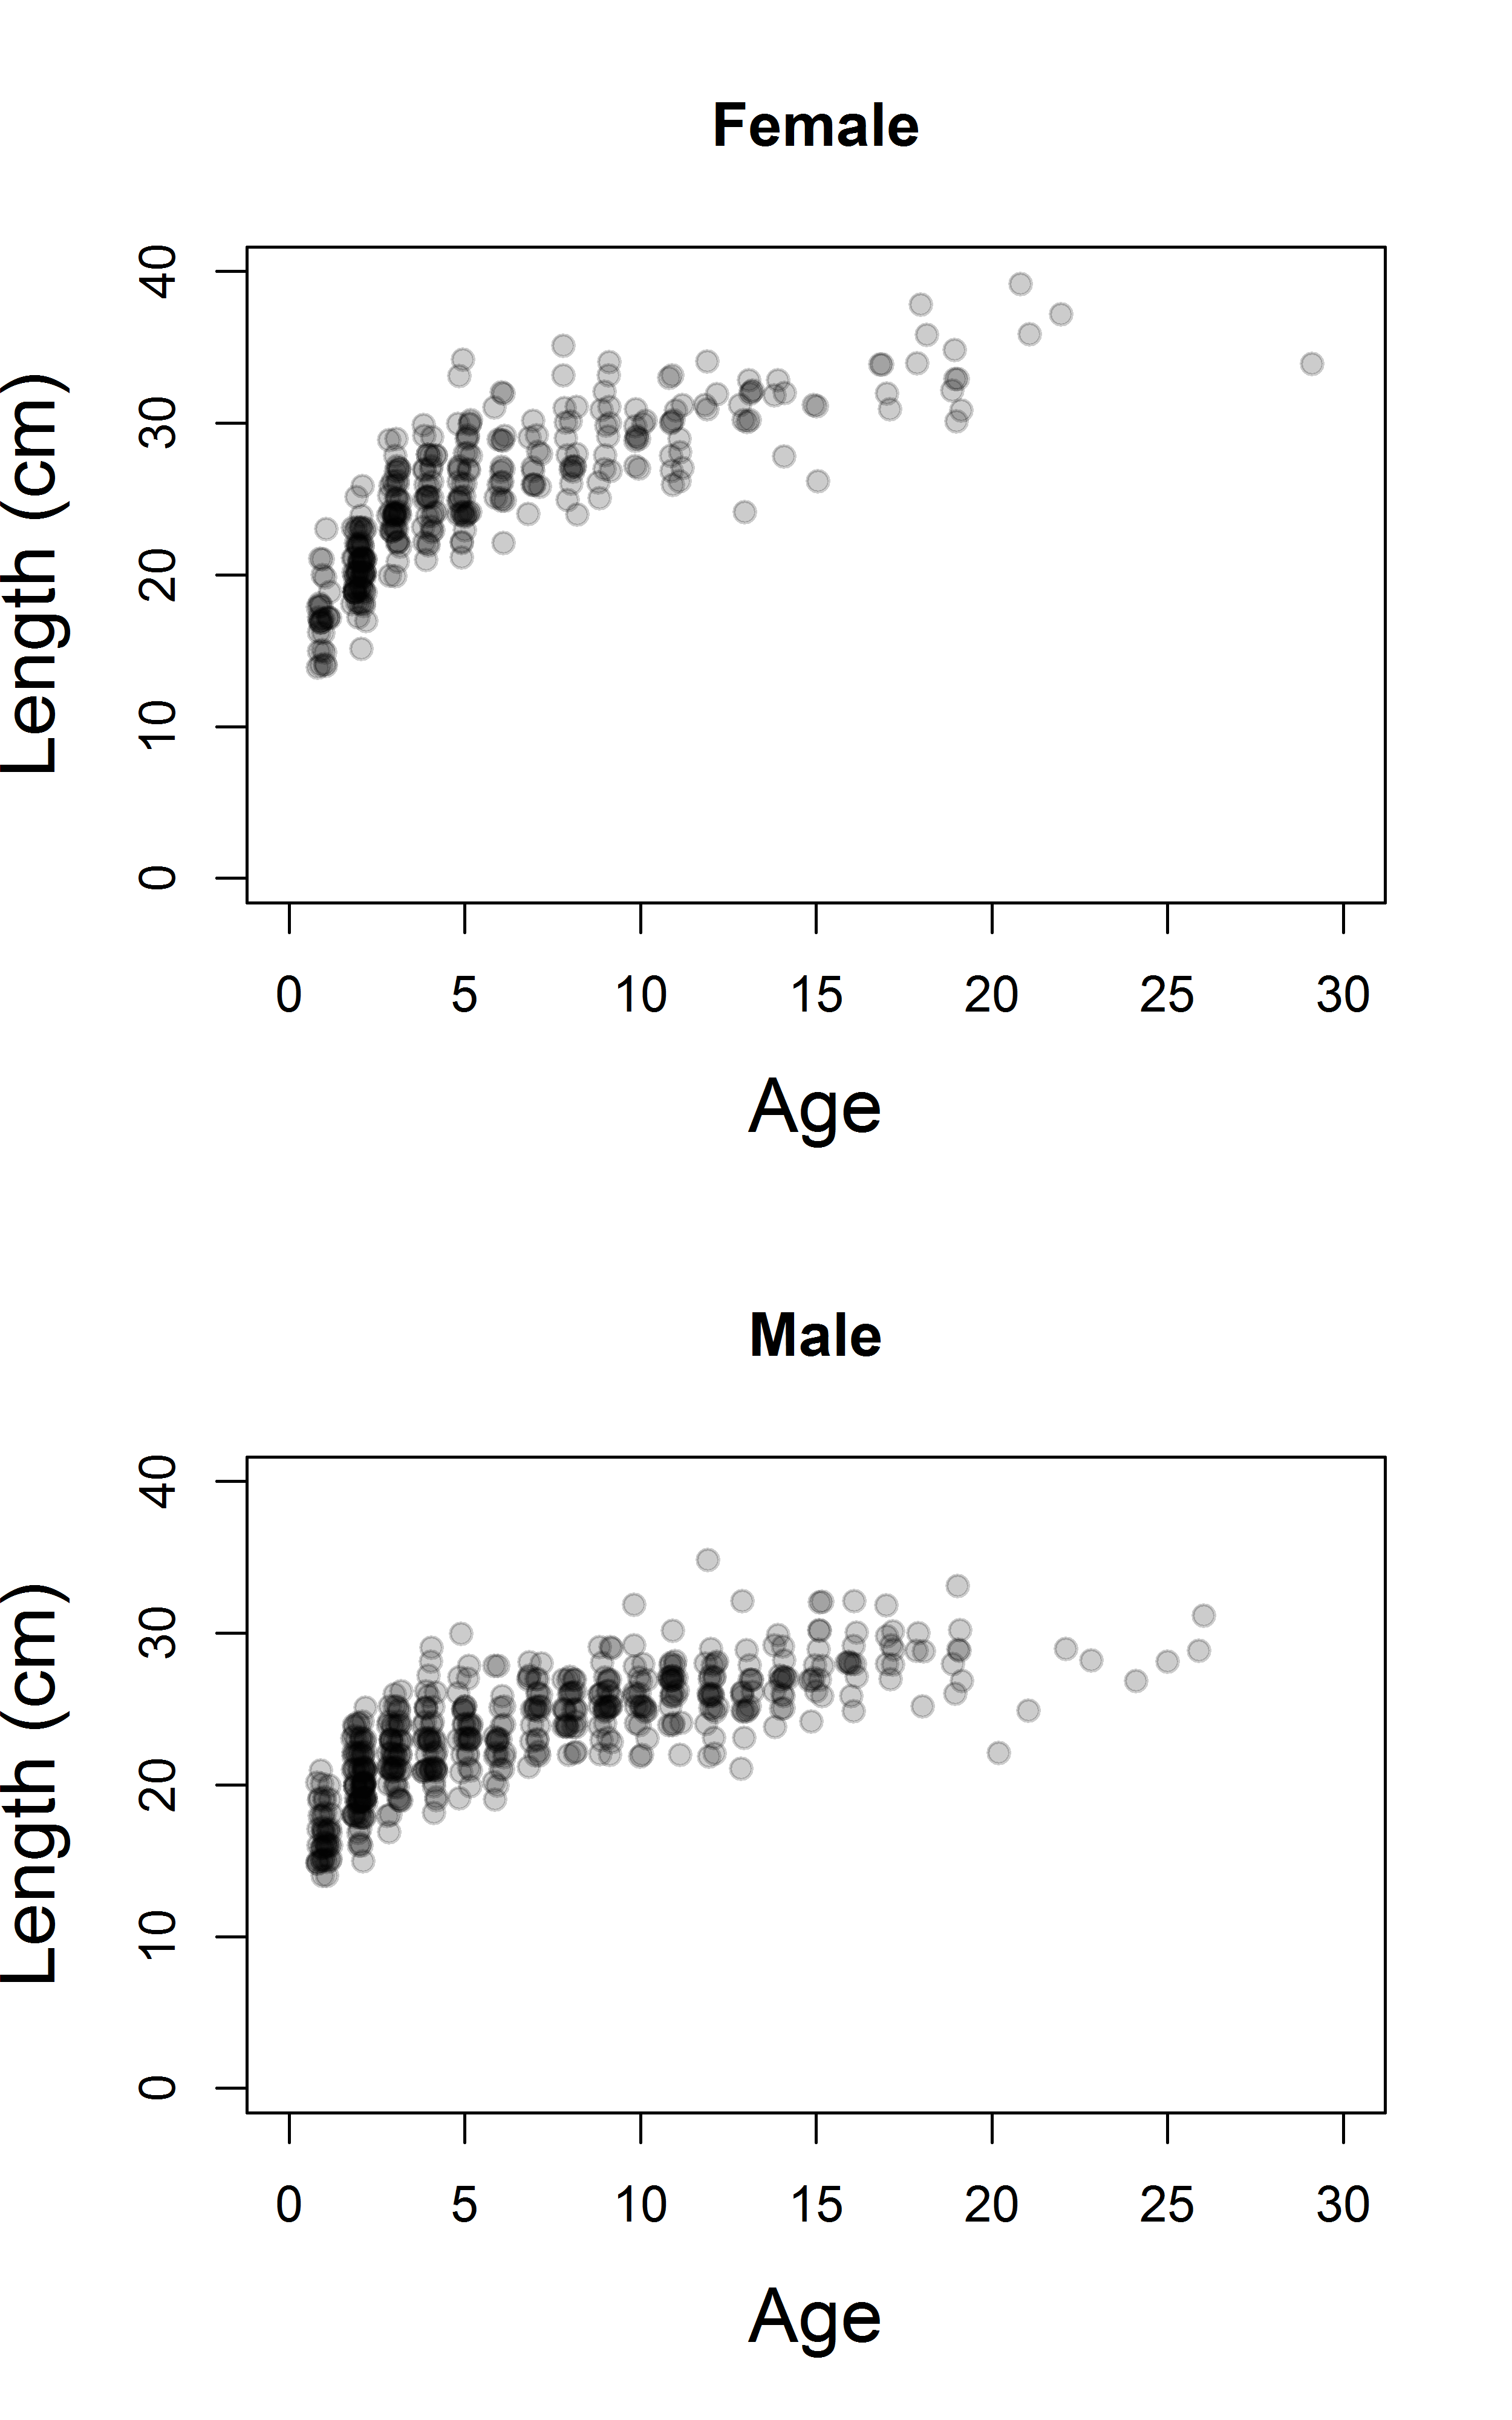
\includegraphics[trim={0 0 0 2cm}, totalheight=0.65\textheight]{Figures/Age_length_bySex.png}
\endcol
 \begincol{.48\textwidth} 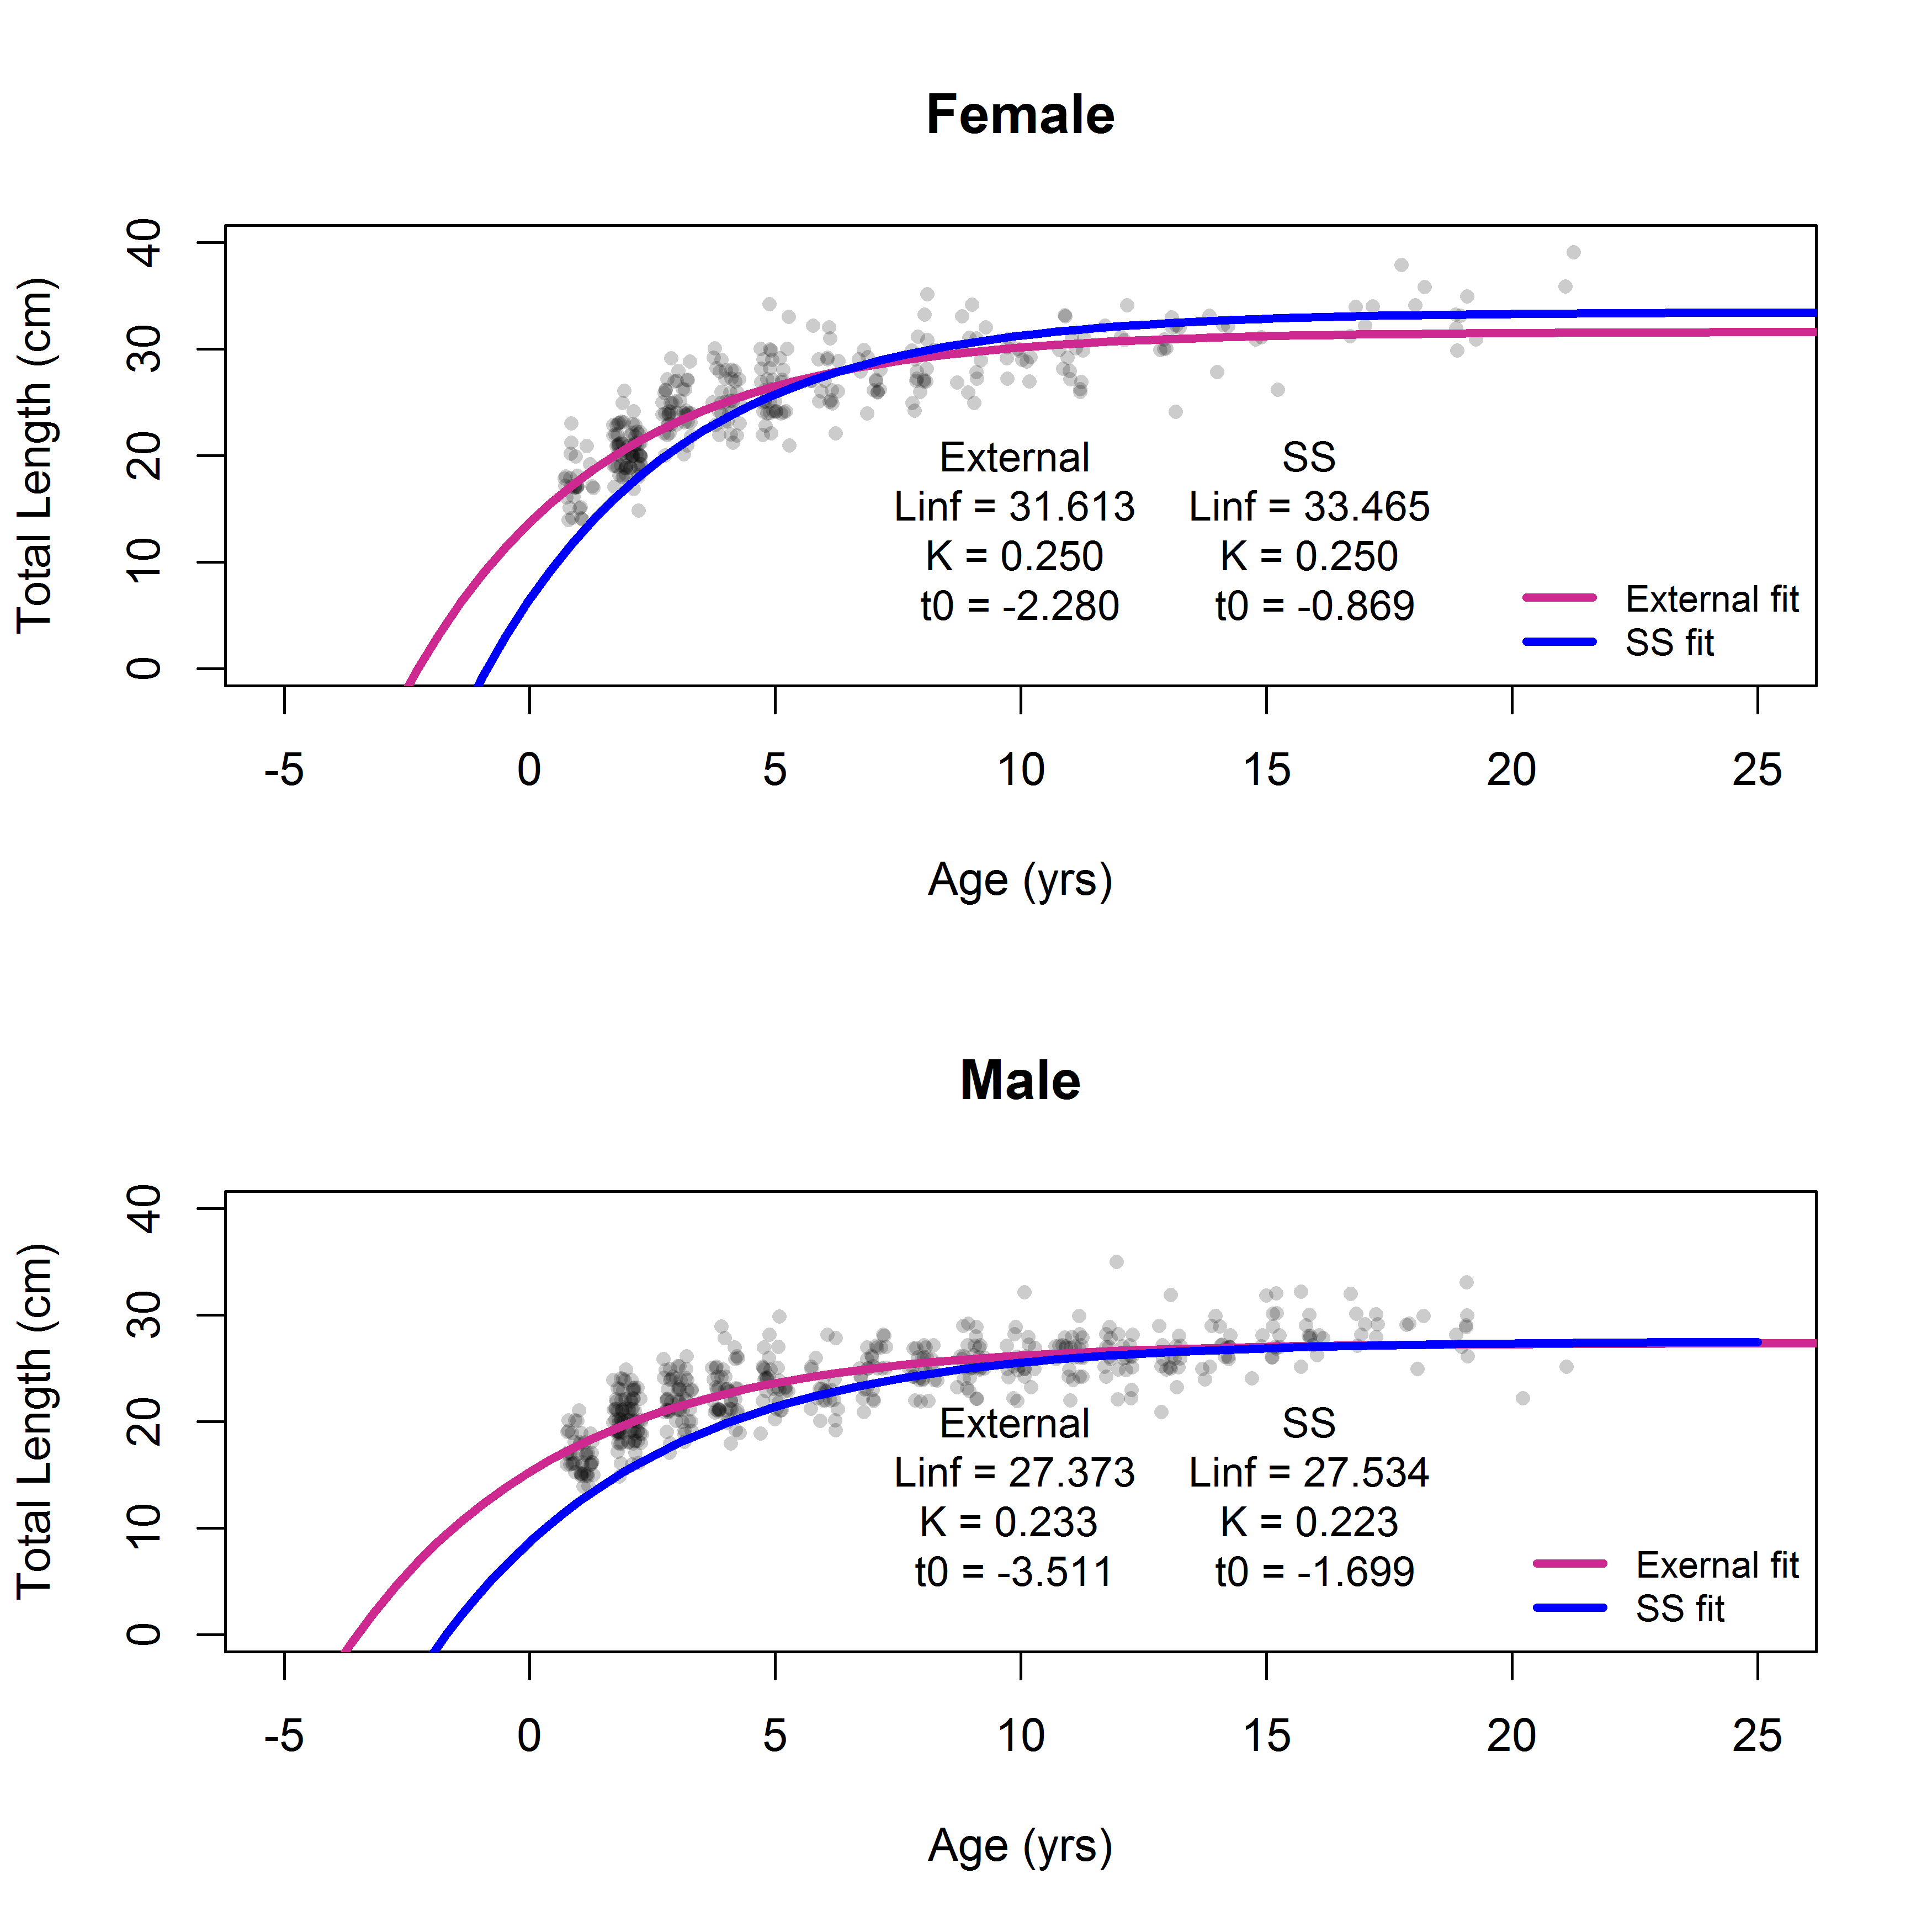
\includegraphics{Figures/vonB_compare.png}
\endcol
\endcols

\end{frame}

\begin{frame}{Length-at-Age}

\begincols
 \begincol{.4\textwidth}
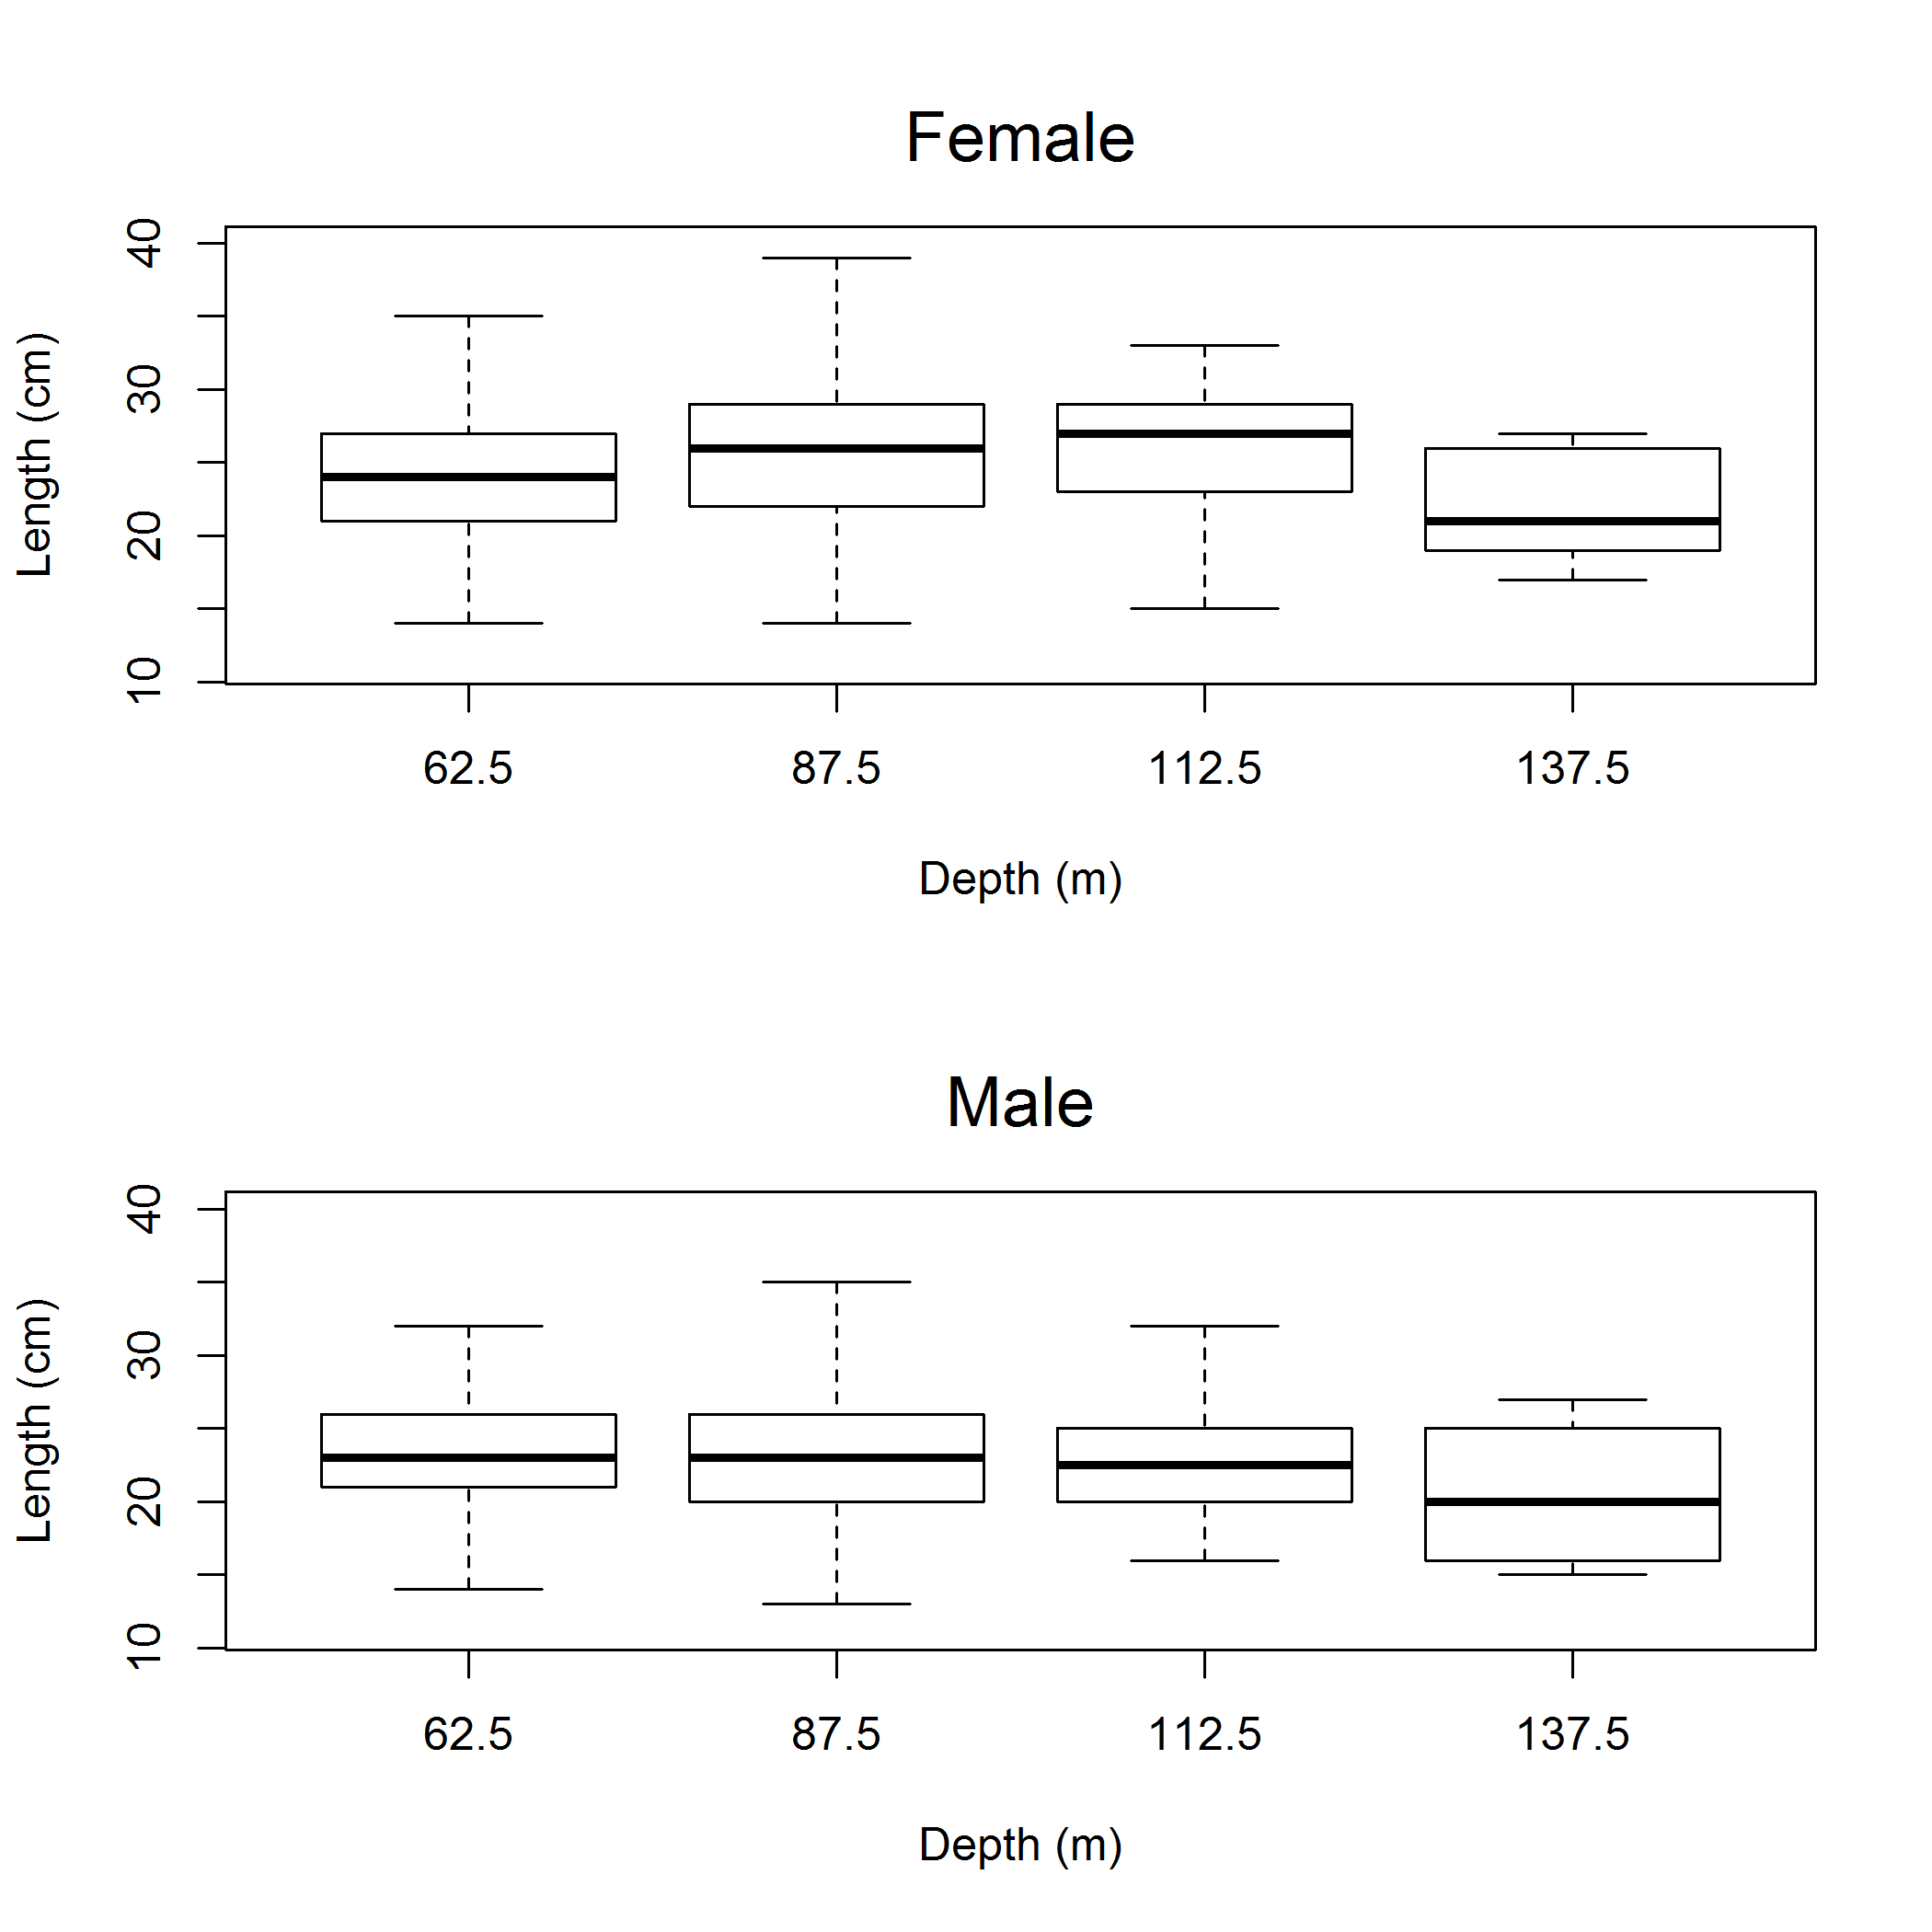
\includegraphics{Figures/NWFSCtrawl_lengthdepth.png} \endcol
\begincol{.48\textwidth}
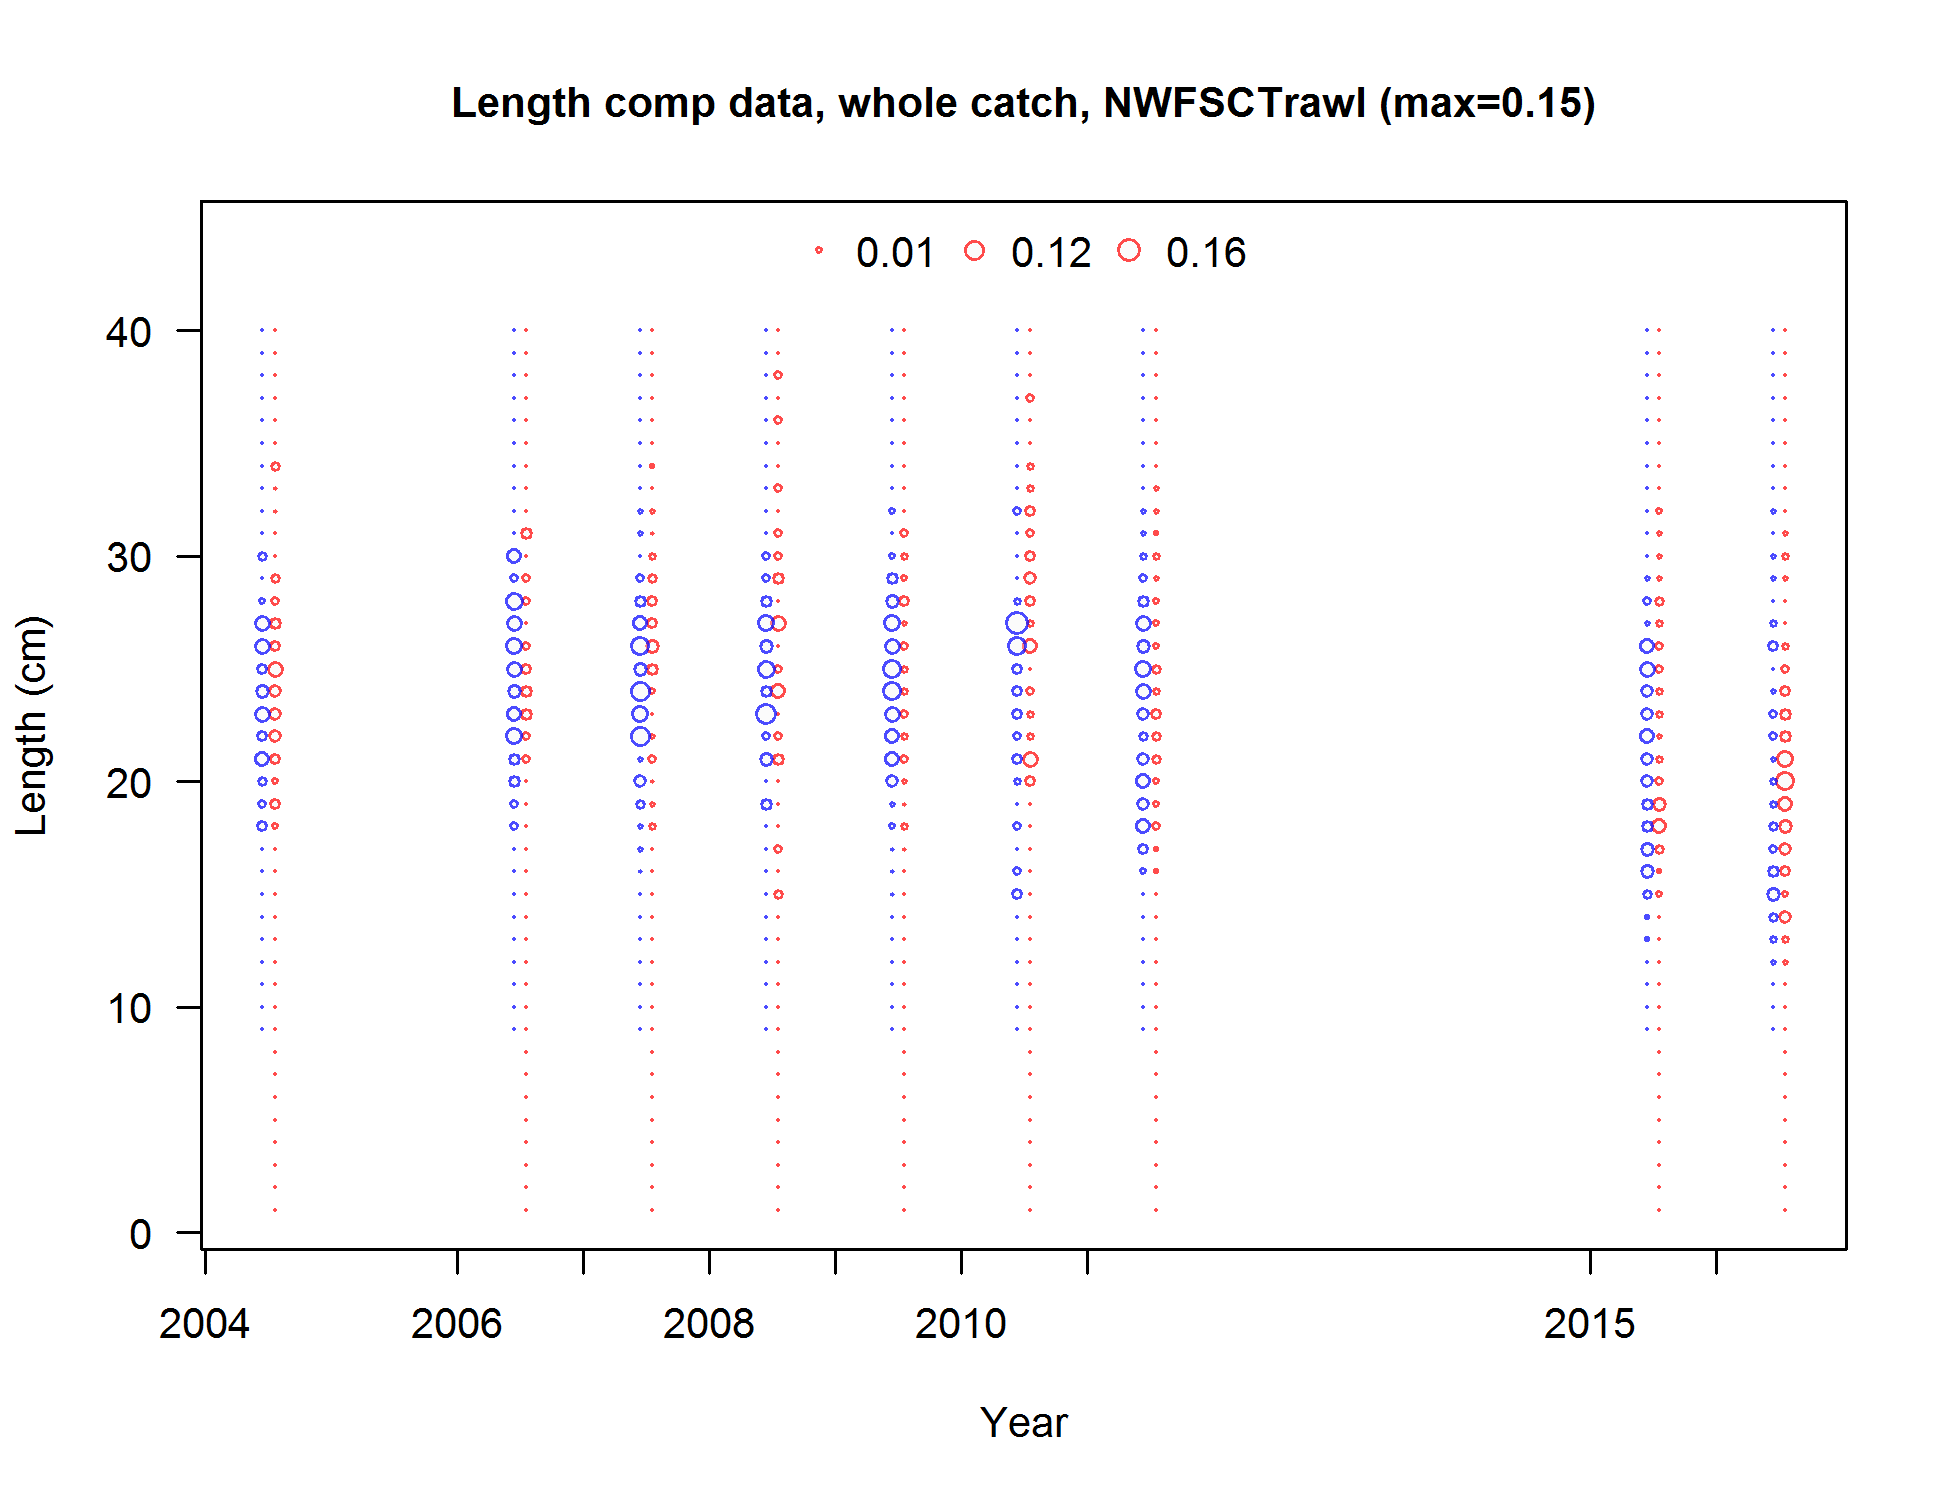
\includegraphics{r4ss/plots_mod1/comp_lendat_bubflt8mkt0.png} \endcol
\endcols

\end{frame}

\section{Model}\label{model}

\begin{frame}{Model Specifications}

\begin{itemize}
\item[$\bullet$] Stock Synthesis version 3.30.05.04
\item[$\bullet$] Model starts in 1916, unfished equilibrium catch prior to that
\item[$\bullet$] Sex-specific growth and mortality with female $M$ fixed at 0.2571 (prior) and male $M$ offset is estimated at -0.2134 (male $M$ = 0.2077)
\begin{itemize}
\item[$\circ$] $M$ fixed at 0.25 for both sexes in 2005 assessment
\end{itemize}
\item[$\bullet$] Steepness fixed at 0.718 (from meta-analysis)
\begin{itemize}
\item[$\circ$] $h$ fixed at 0.7 in 2005 assessment
\end{itemize}
\item[$\bullet$] Maximum age of 21
\item[$\bullet$] One cm length bins
\item[$\bullet$] Recruitment deviations estimated
\end{itemize}

\end{frame}

\begin{frame}{Selectivity}

\begin{itemize}
\item[$\bullet$] Time blocks
\begin{itemize}
\item[$\circ$] Commercial fleet: 1916-1999 and 2000-2016 (10-in. minimum size limit as of 2000)
\item[$\circ$] Recreational fleets: 1916-2000 (few regulations), 2001-2005 (fishery closures), 2006-2016 (consistent regulations)
\end{itemize}
\item[$\bullet$] Double normal except for the impingement survey (Selectivity = 1.0 for all ages)
\item[$\bullet$] Fisheries selectivity parameters estimated for commercial hook-and-line, receational private, recreational party/charter, and recreational discard fleets
\end{itemize}

\end{frame}

\begin{frame}{Selectivity}

\begin{itemize}
\item[$\bullet$] Commercial gillnet and trawl fleets mirrored to the commercial hook-and-line fleet
\item[$\bullet$] Recreational CPFV onboard observer retained catch mirrored to the recreational party/charter fleet selectivity (same boats)
\item[$\bullet$] Survey selectivity parameters estimated for the POTW and NWFSC trawl surveys
\item[$\bullet$] The gillnet survey and Bight trawl survey mirrored to the POTW selectivity 
\end{itemize}

\centering
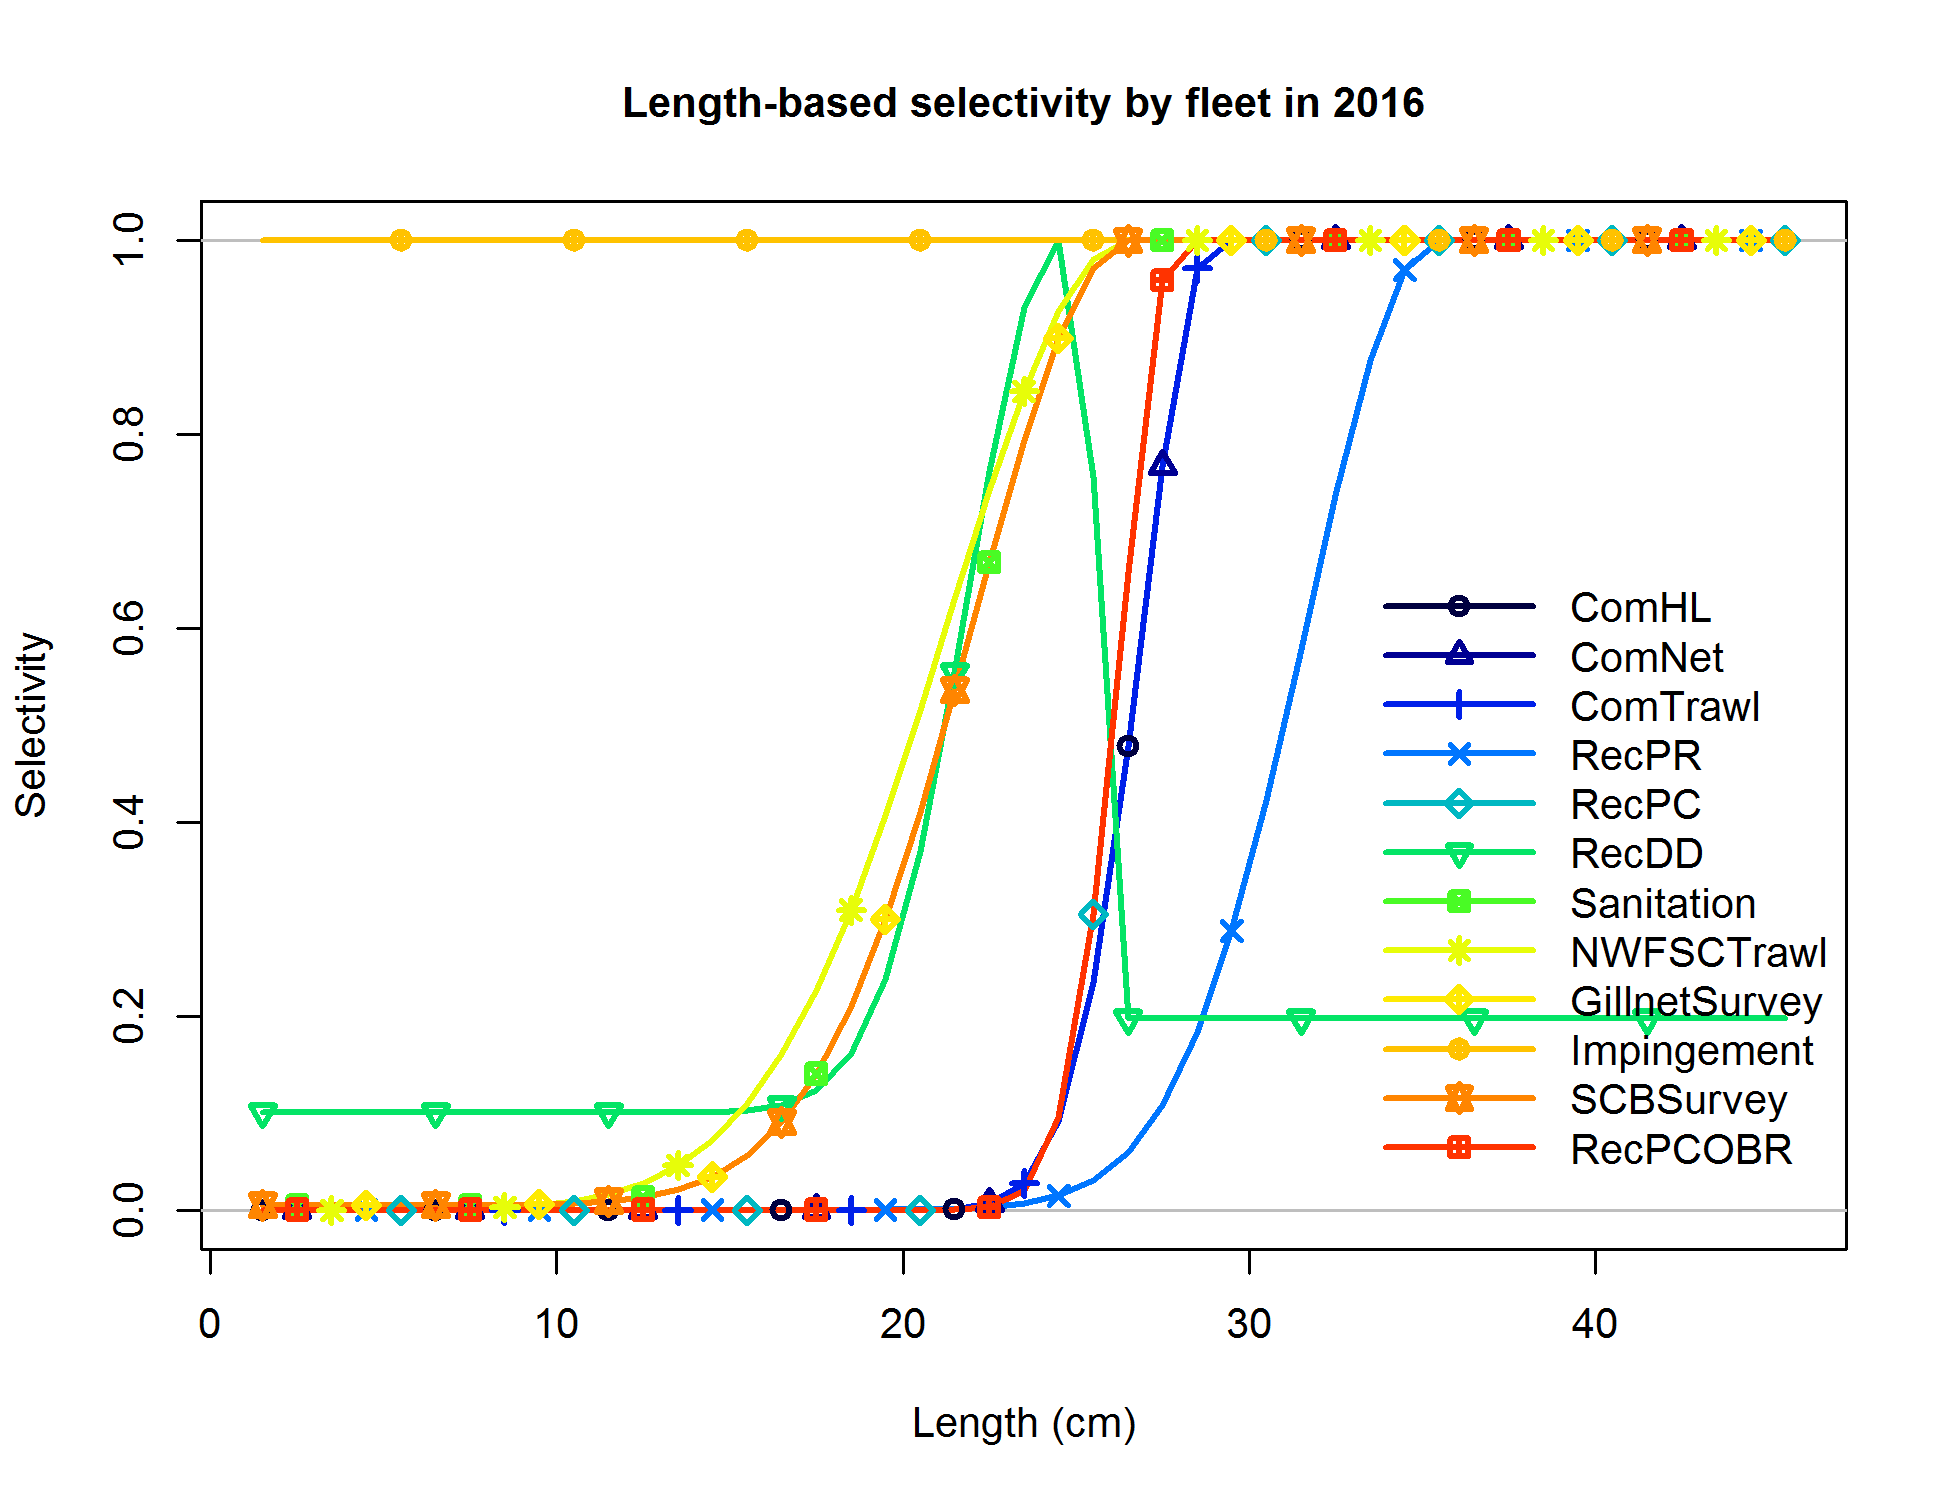
\includegraphics[height=4cm]{r4ss/plots_mod1/sel01_multiple_fleets_length1.png}

\end{frame}

\begin{frame}{Selectivity}

\begincols
 \begincol{.5\textwidth}
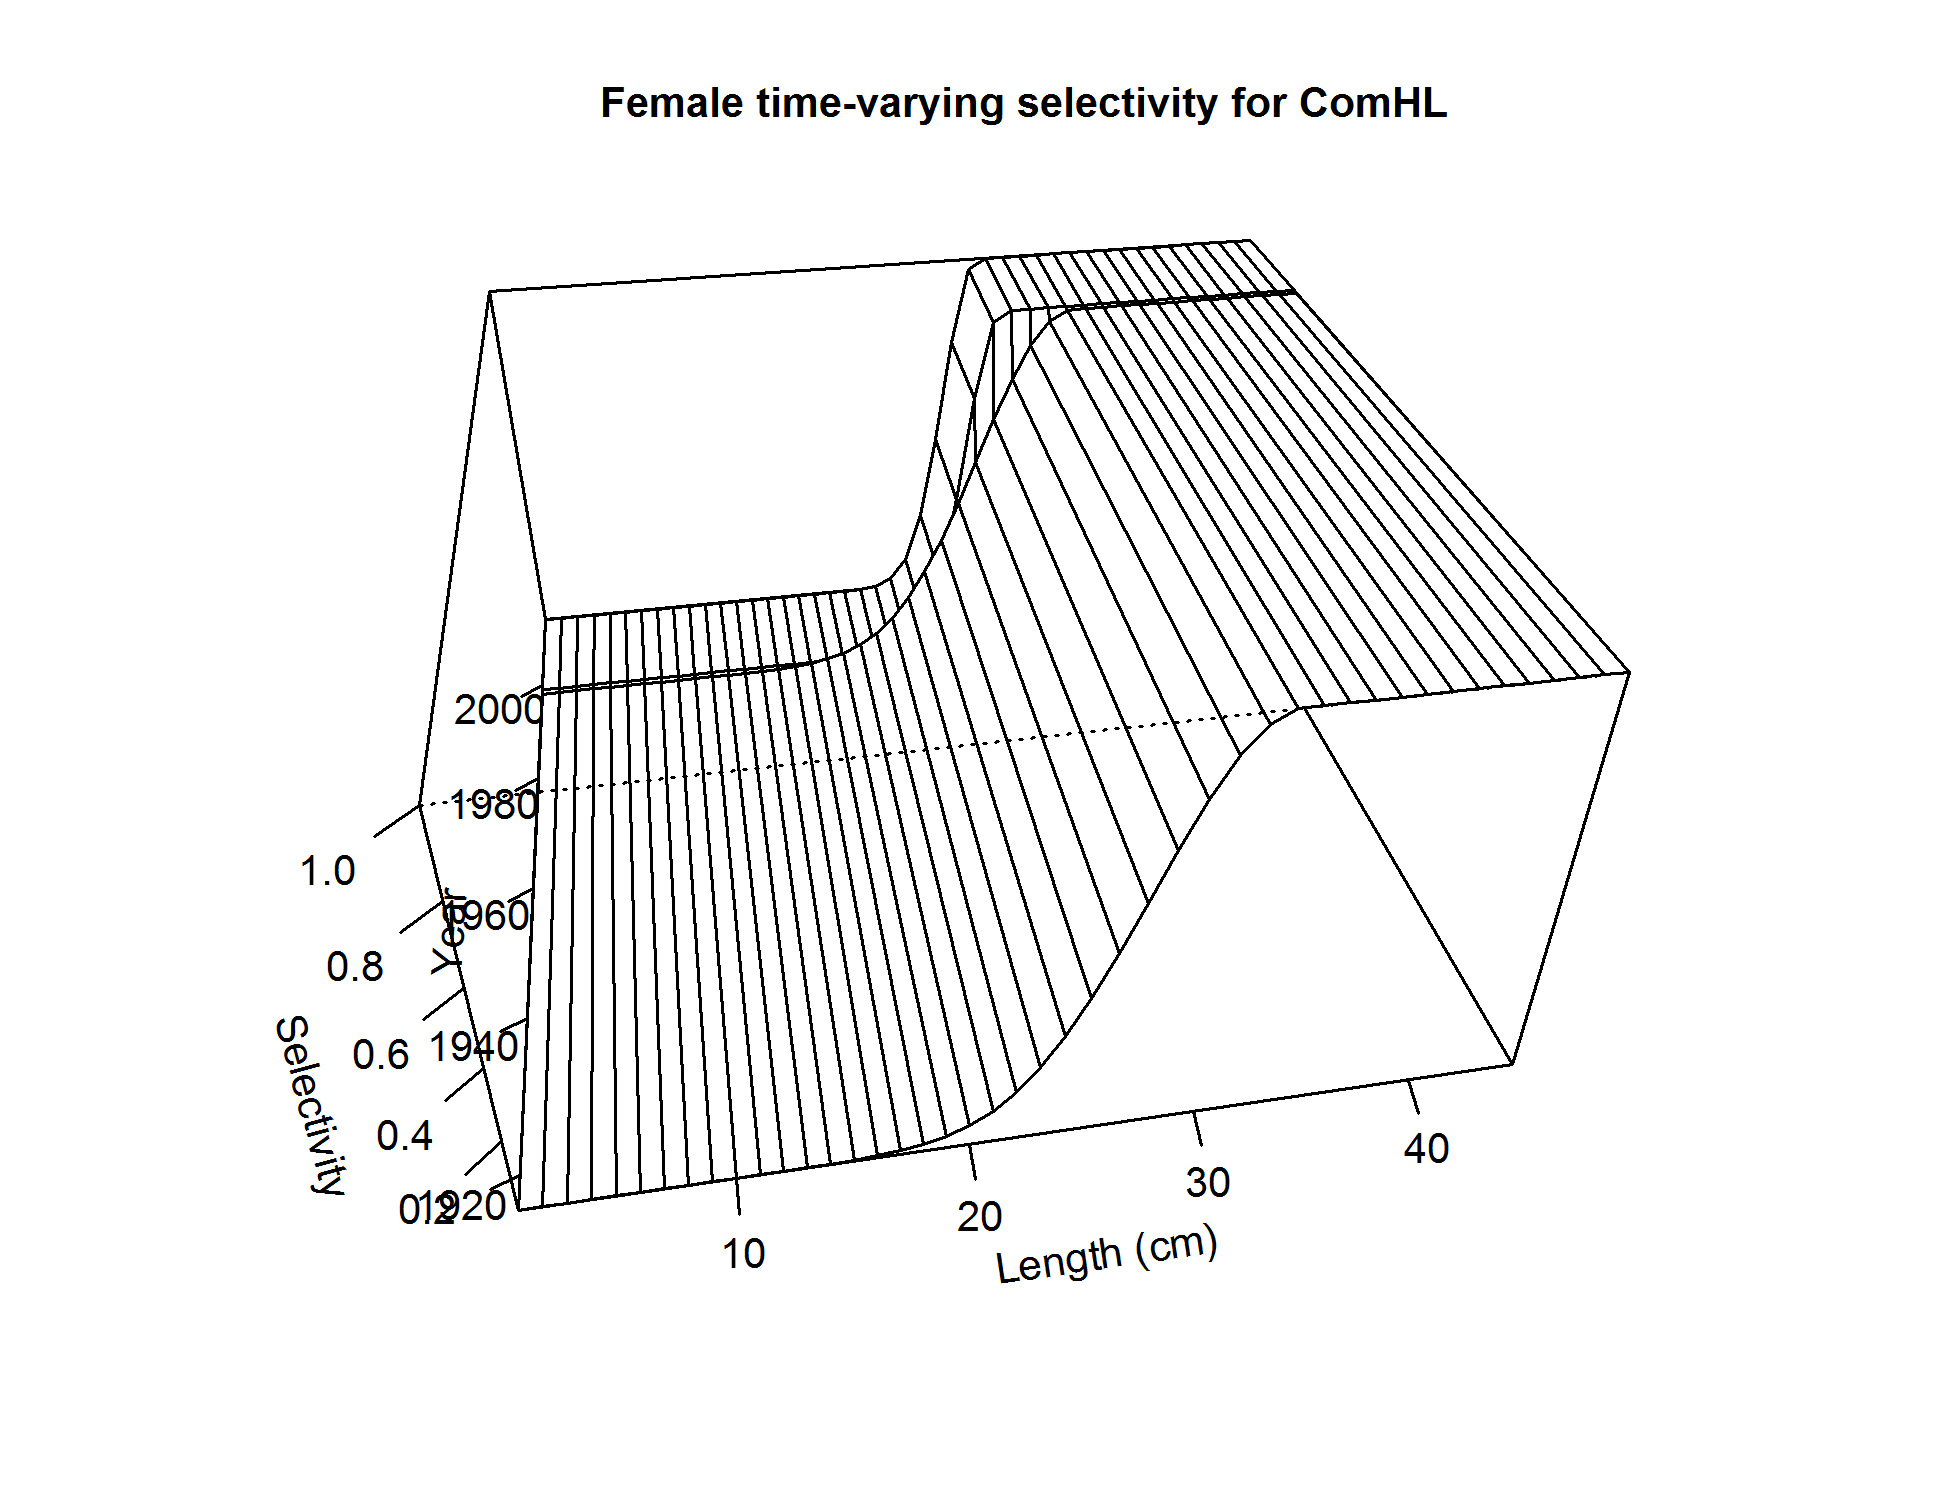
\includegraphics[height=4cm]{r4ss/plots_mod1/sel03_len_timevary_surf_flt1sex1.png}

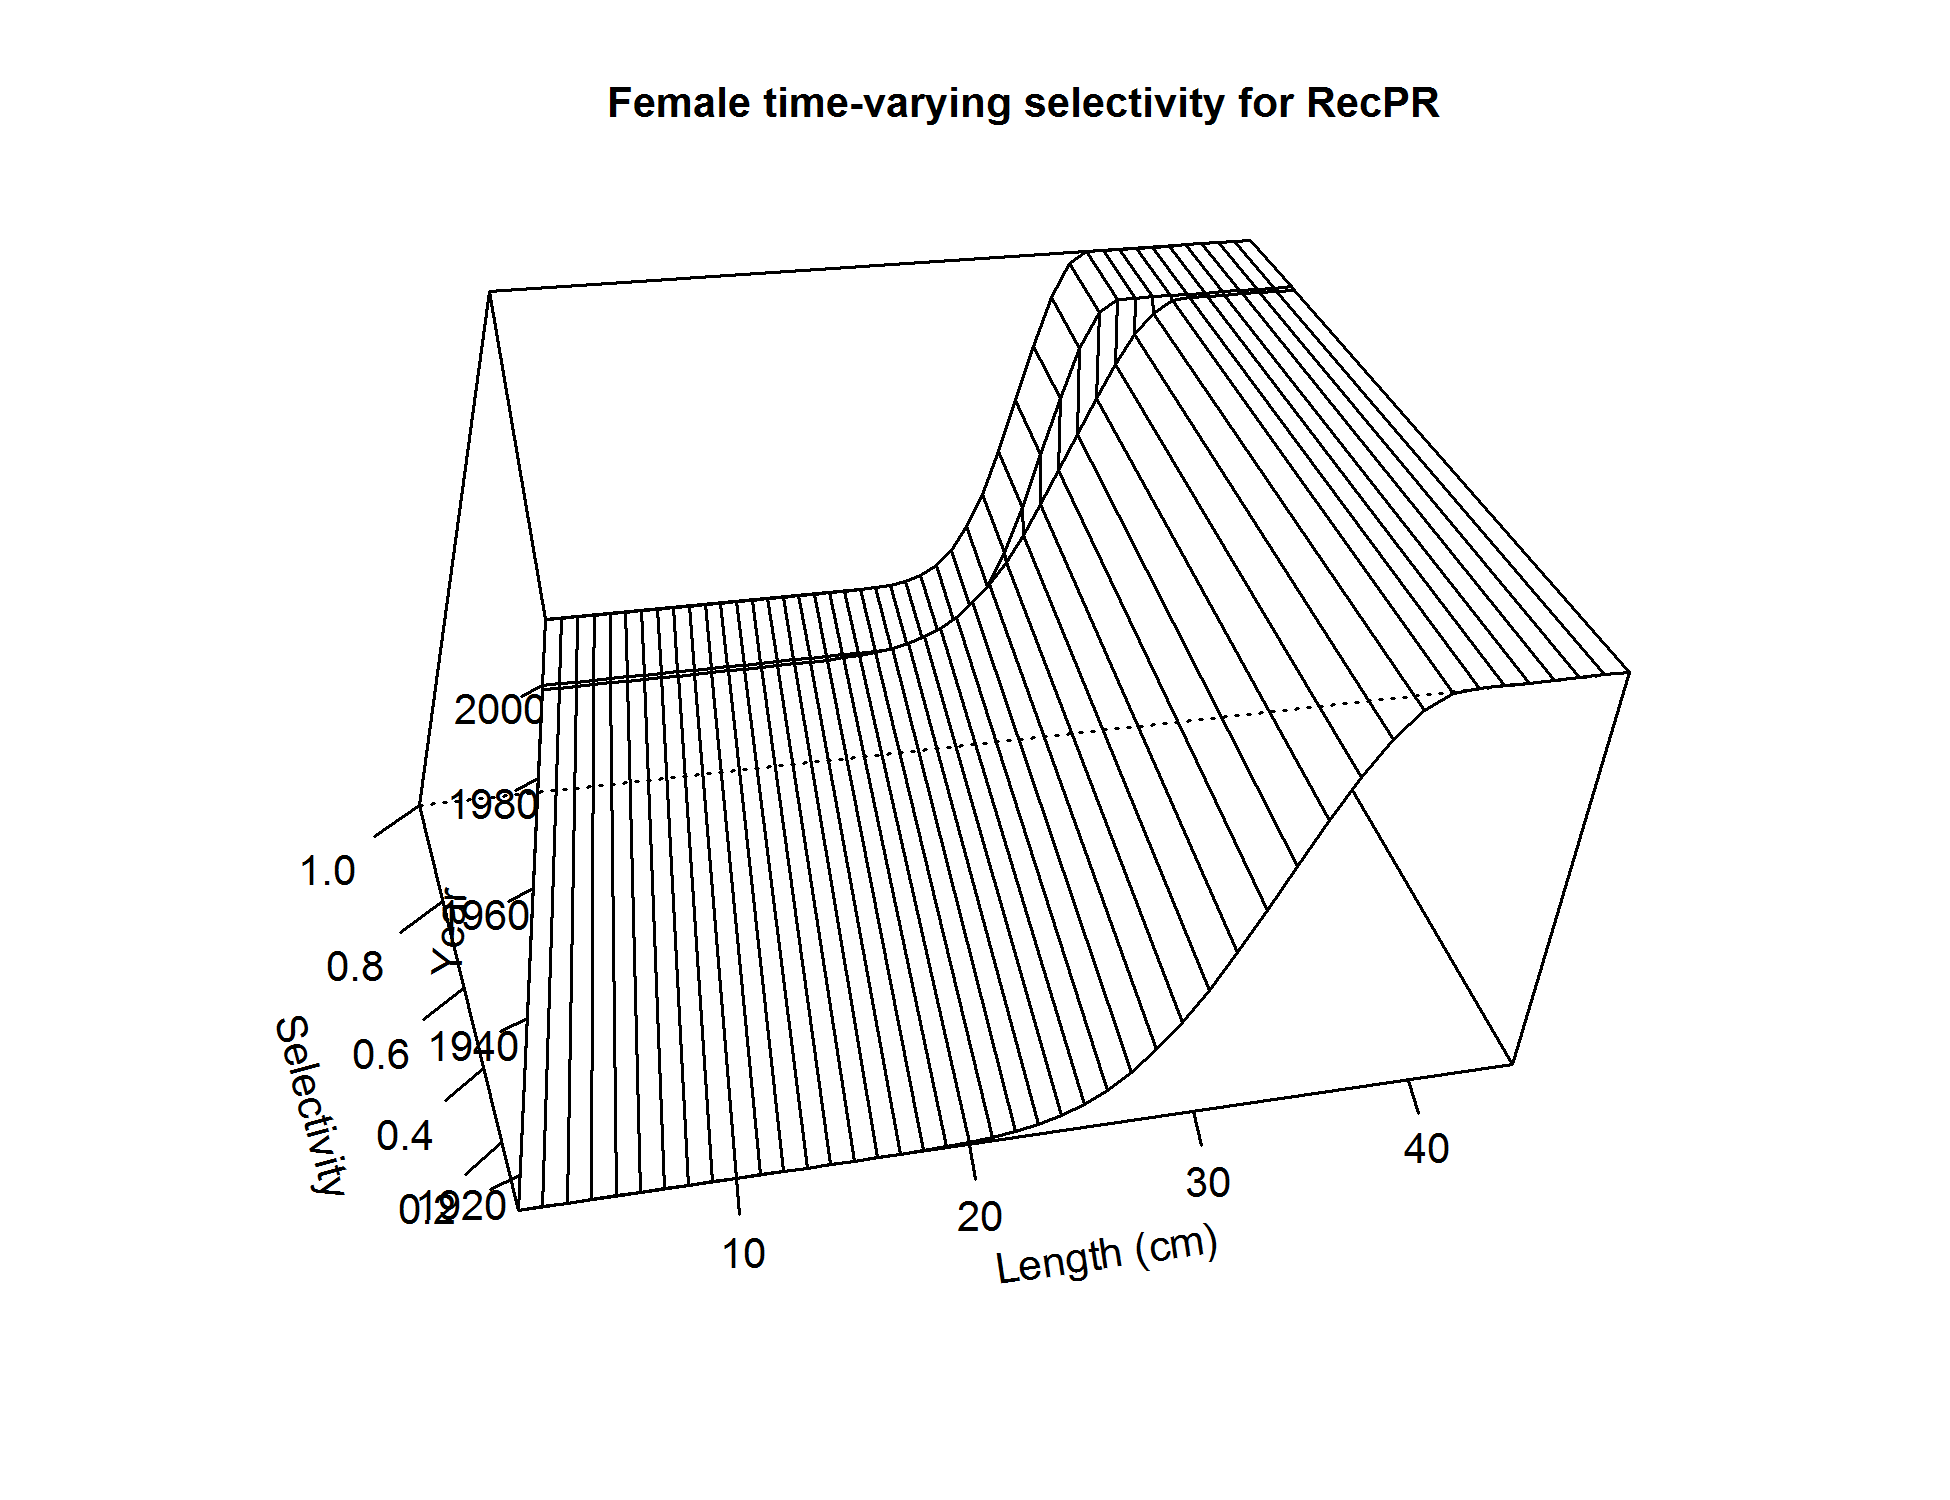
\includegraphics[height=4cm]{r4ss/plots_mod1/sel03_len_timevary_surf_flt4sex1.png}
\endcol
 \begincol{.5\textwidth}

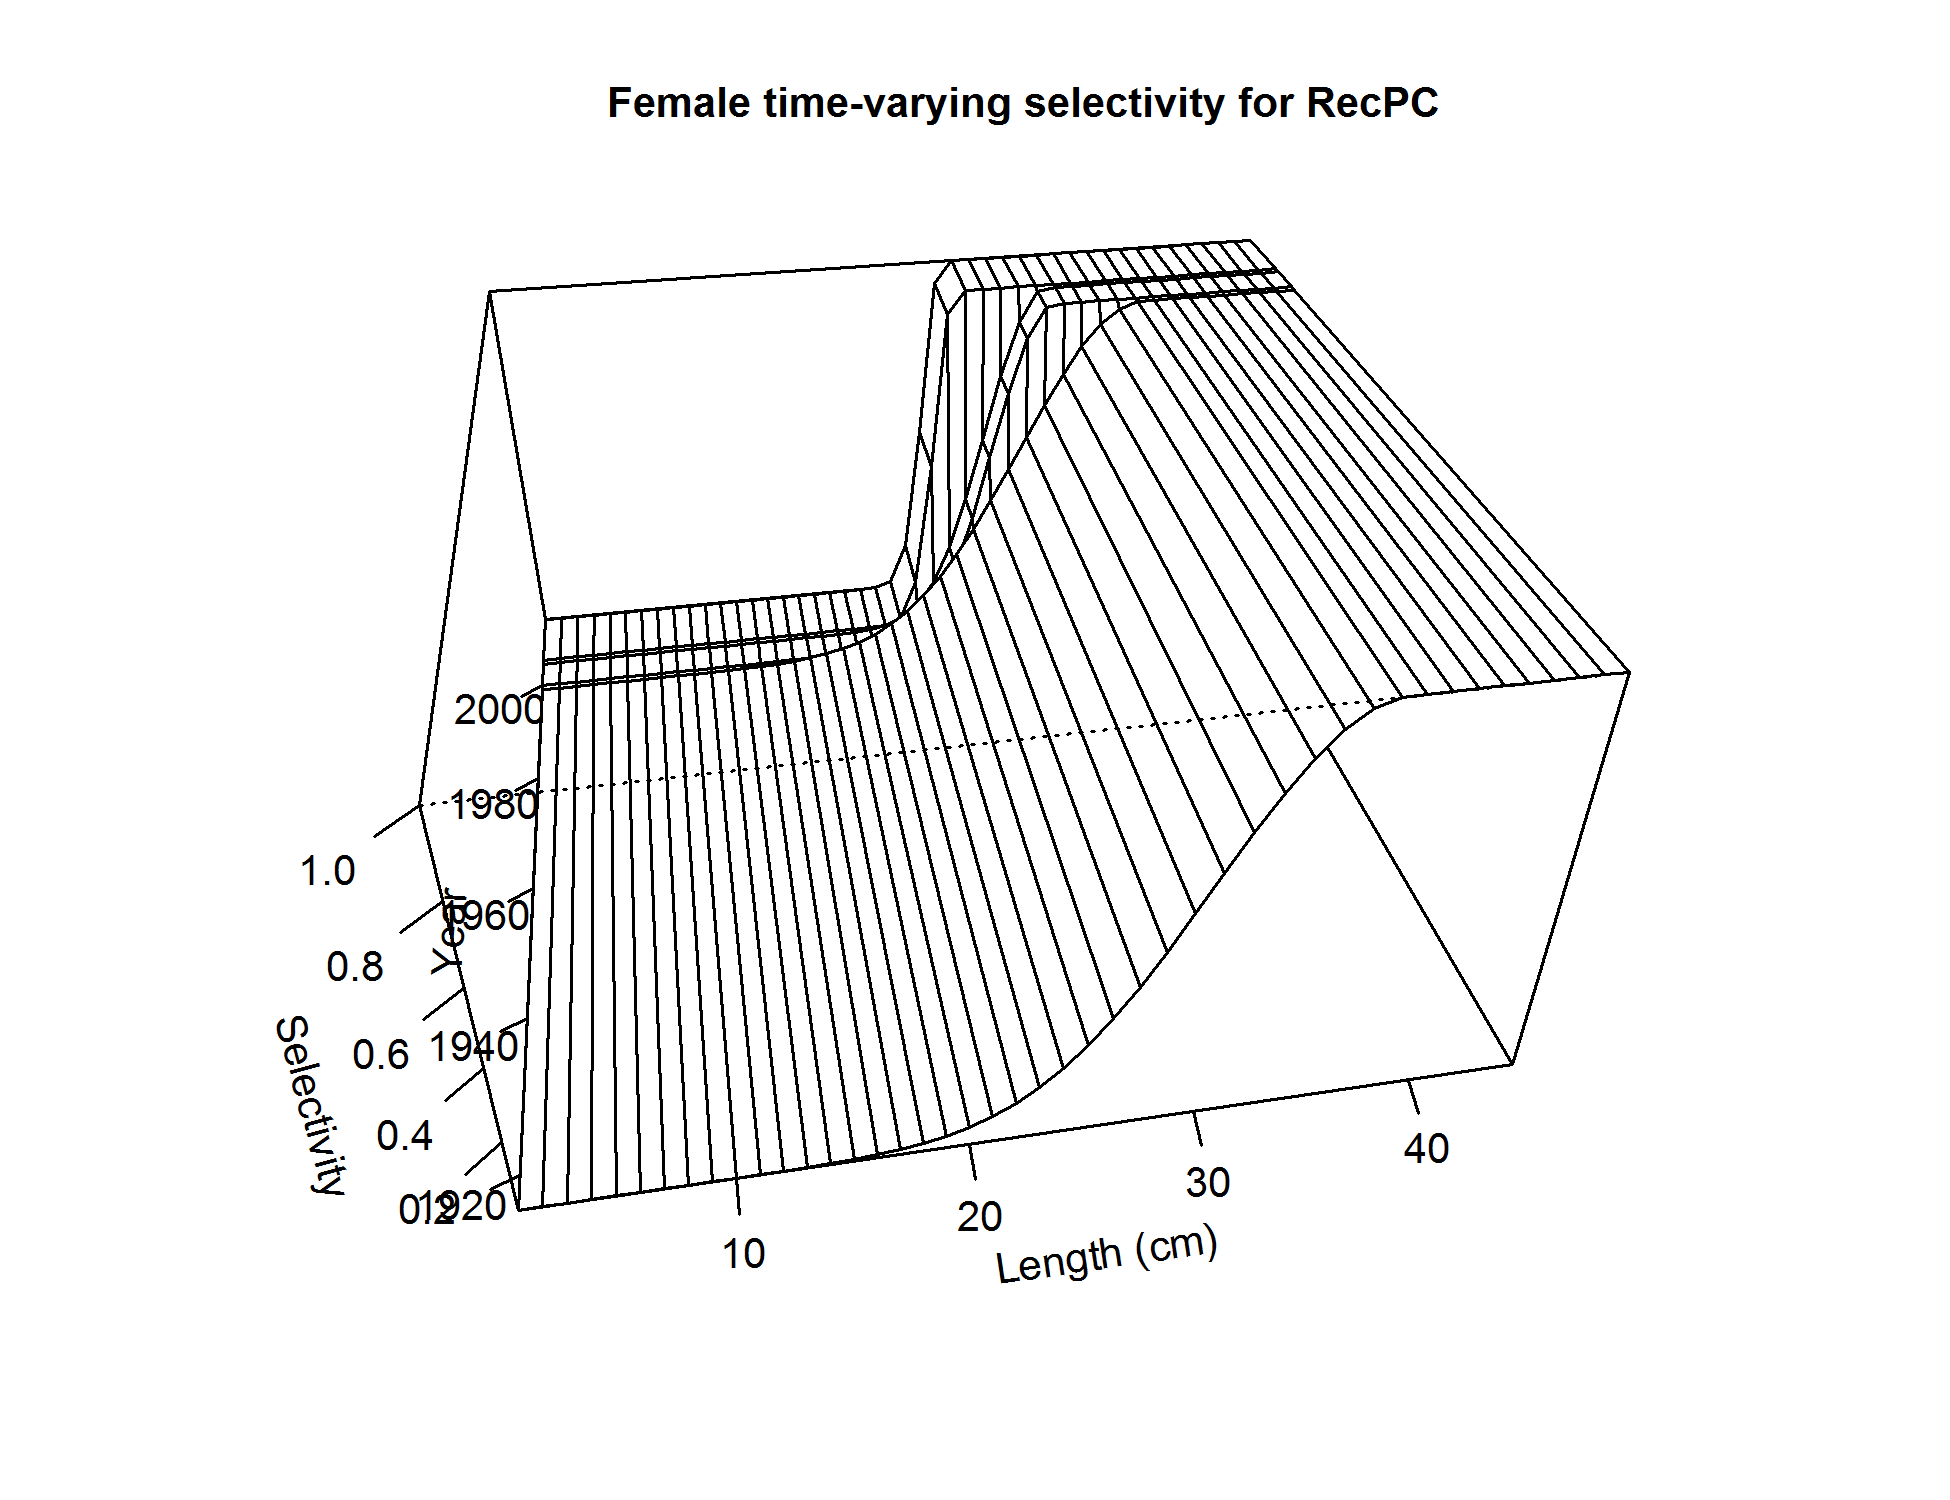
\includegraphics[height=4cm]{r4ss/plots_mod1/sel03_len_timevary_surf_flt5sex1.png}\\
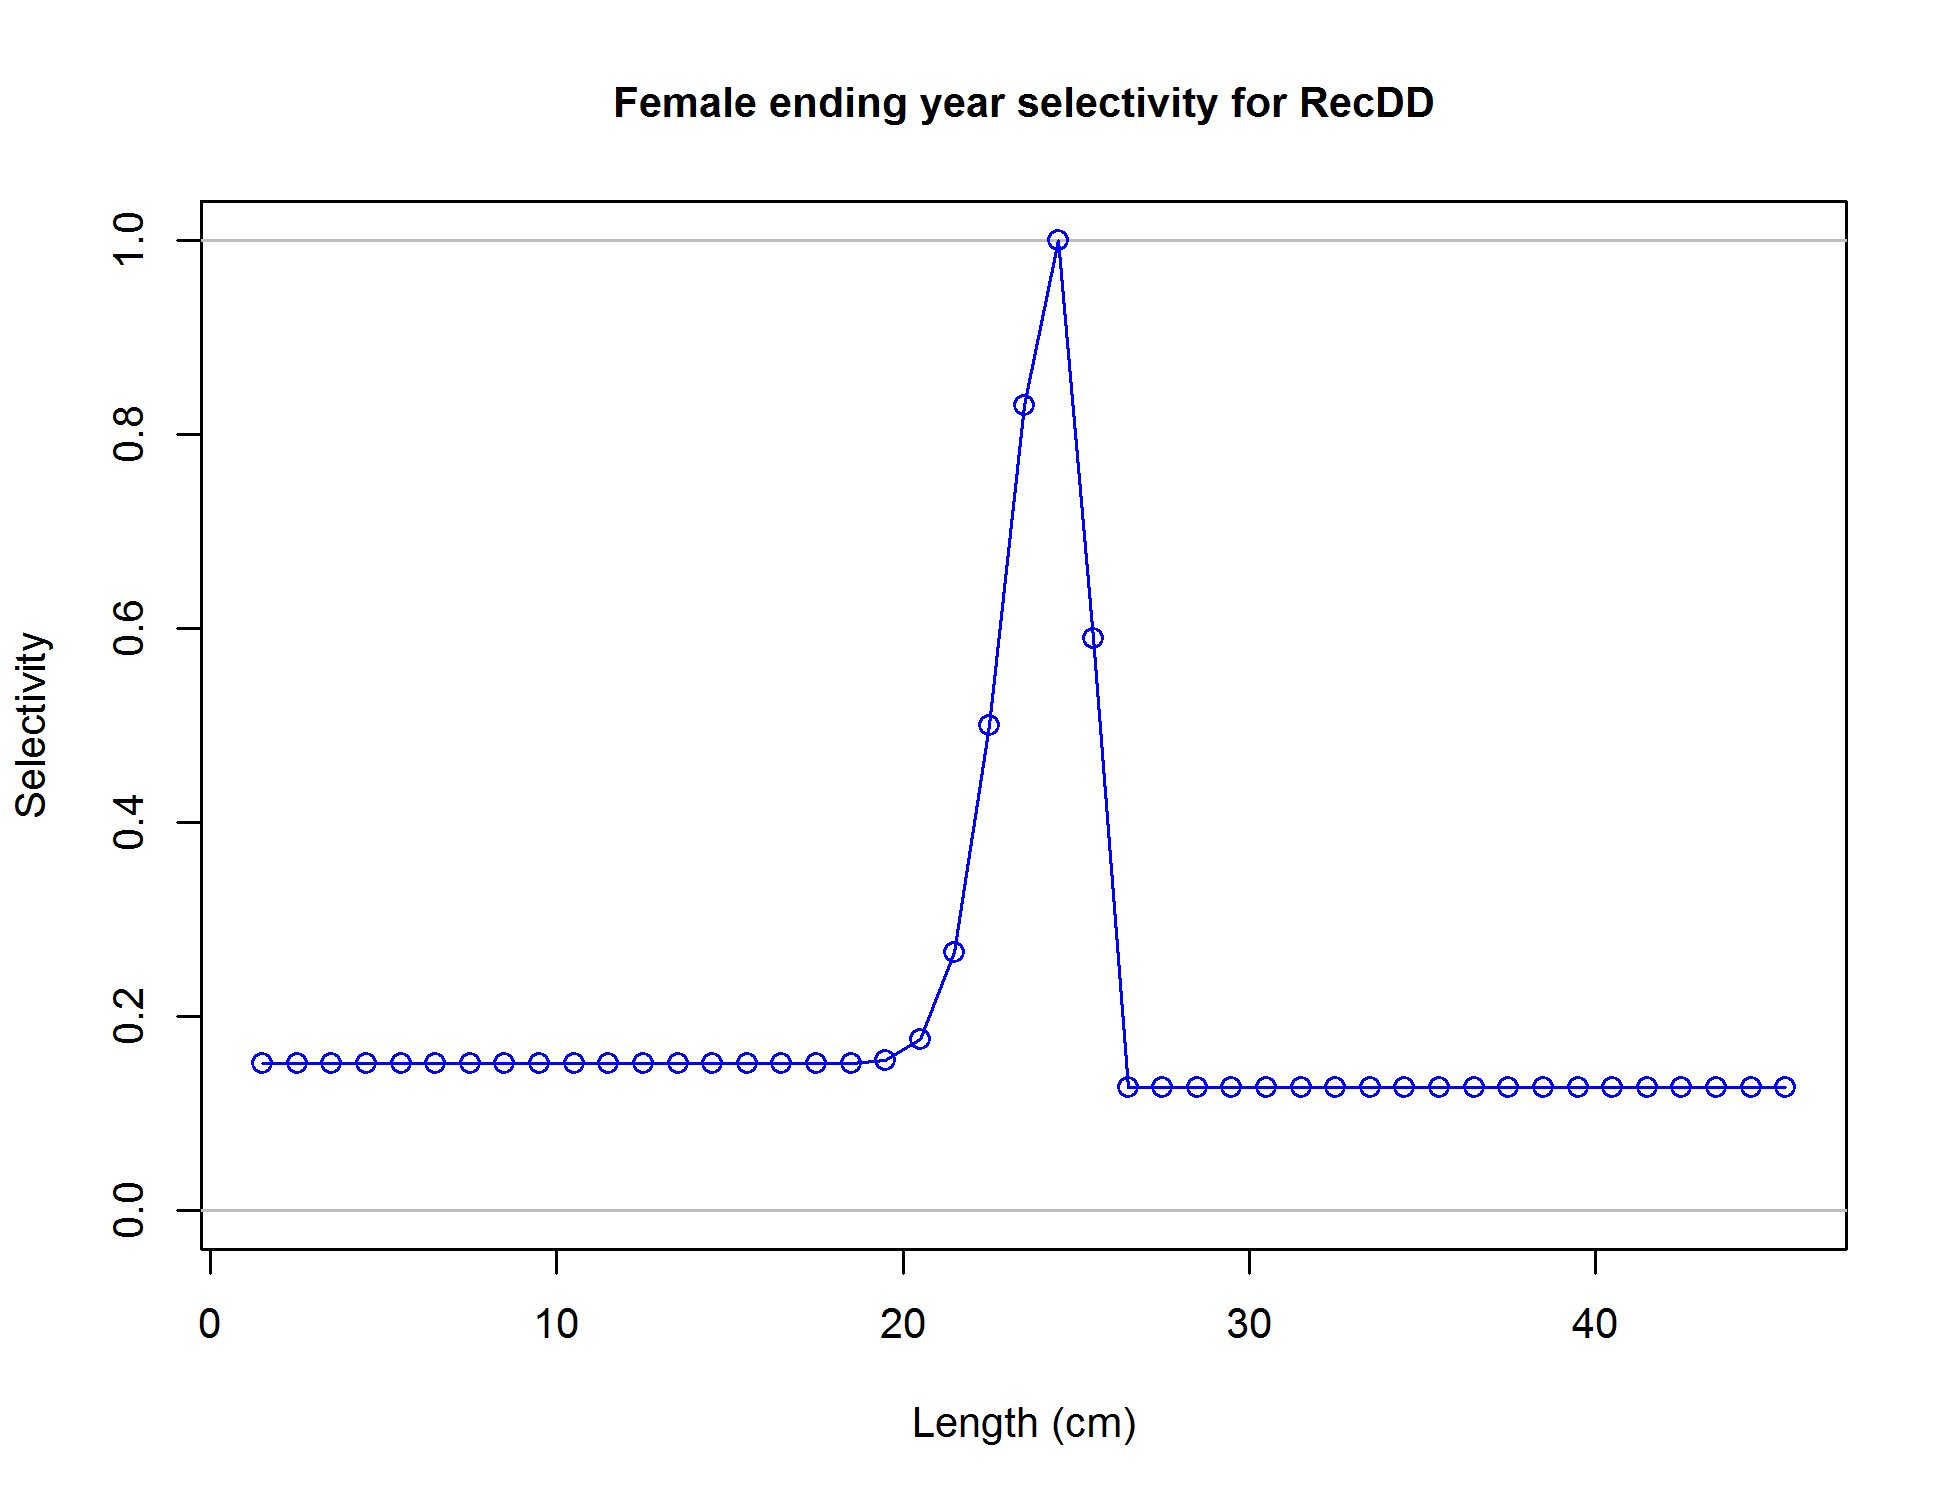
\includegraphics[height=4cm]{r4ss/plots_mod1/sel09_len_flt6sex1.png}\\
\endcol
\endcols

\end{frame}

\begin{frame}{Gear Selectivity}

\begincols
 \begincol{.5\textwidth}
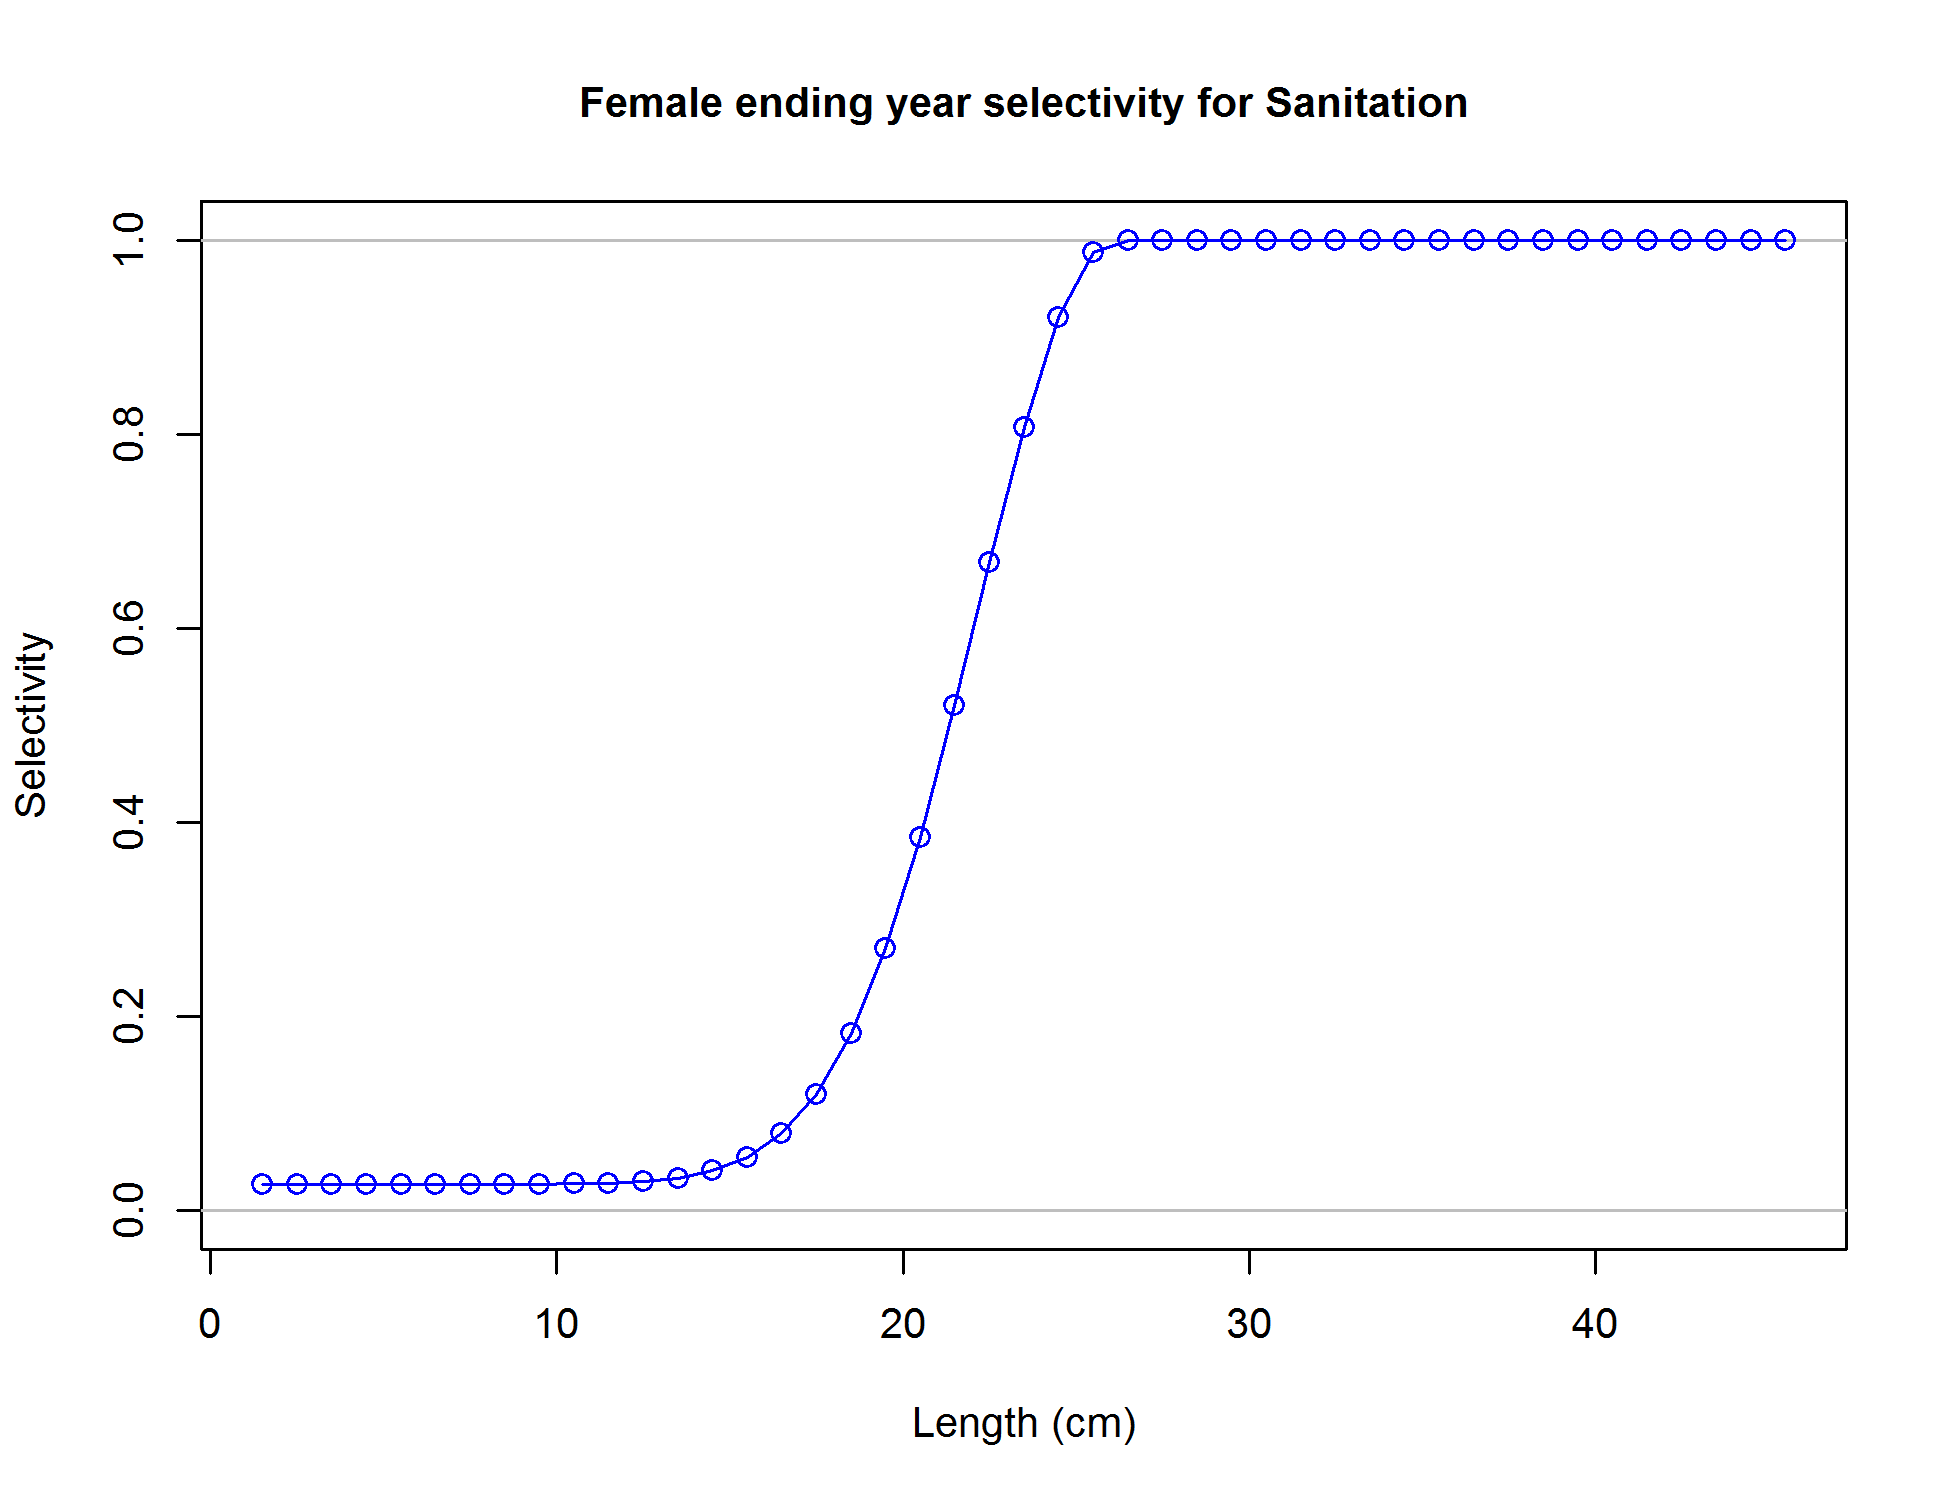
\includegraphics[height=4cm]{r4ss/plots_mod1/sel09_len_flt7sex1.png}

\endcol
 \begincol{.5\textwidth}
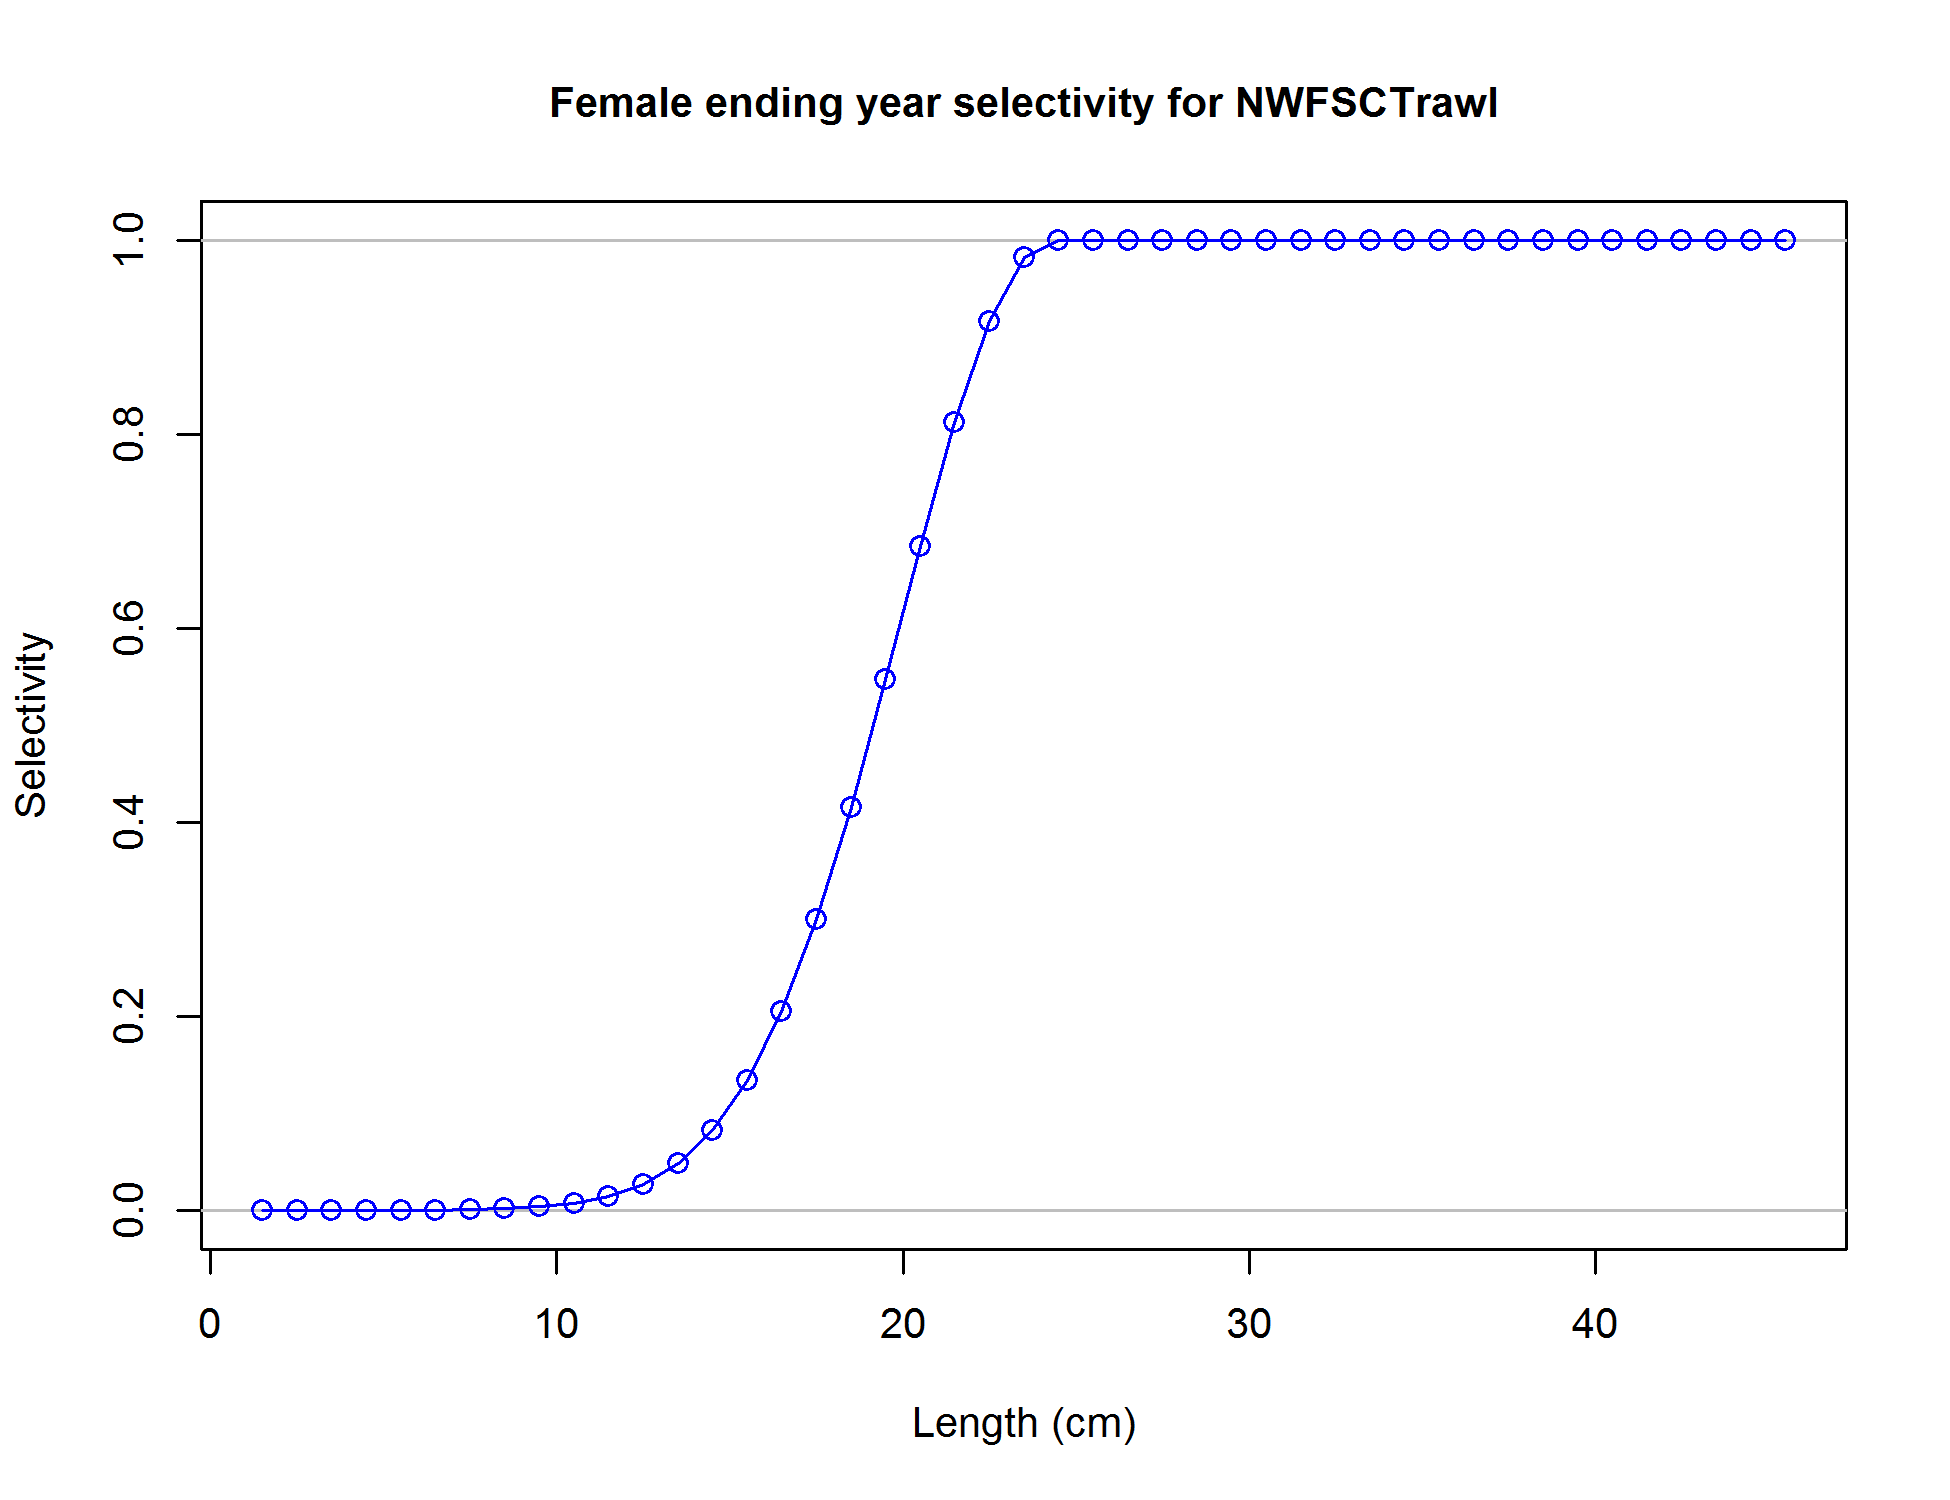
\includegraphics[height=4cm]{r4ss/plots_mod1/sel09_len_flt8sex1.png}
\endcol
\endcols

\end{frame}

\begin{frame}{Data Weighting}

\begin{itemize}
\item[$\bullet$] Extra SD estimated for indices
\item[$\bullet$] Francis weighting applied to length and age data
\item[$\bullet$] Conducted sensitivities to no weighting and harmonic means
\end{itemize}

\begincols
 \begincol{.5\textwidth}
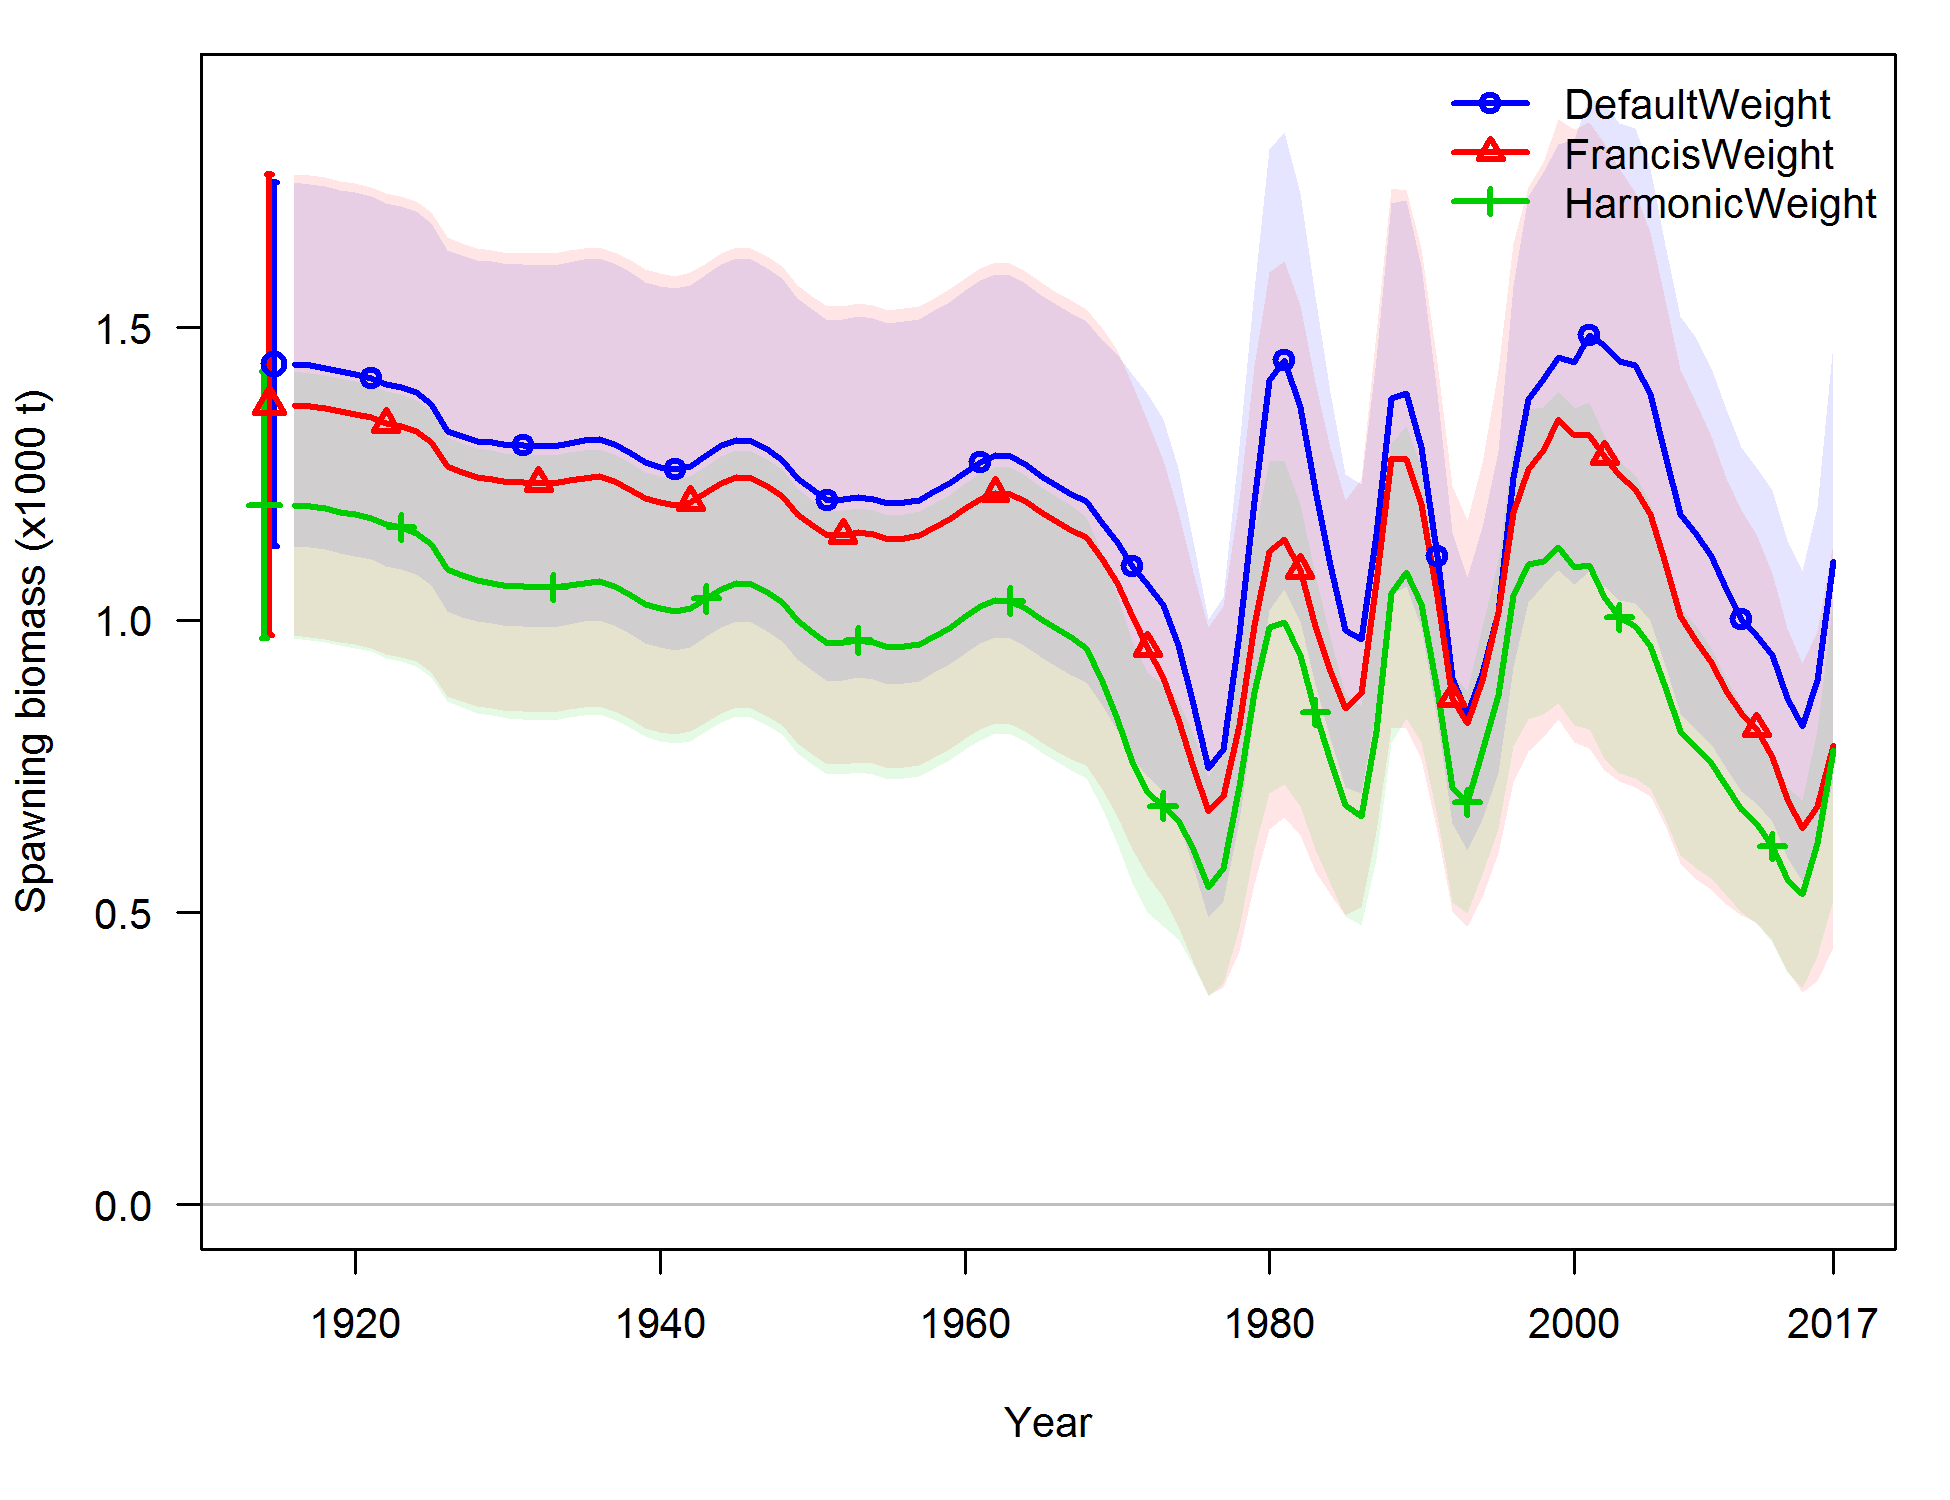
\includegraphics[height=4cm]{Figures/Data_weighting_spawnb.png} \endcol
 \begincol{.5\textwidth}
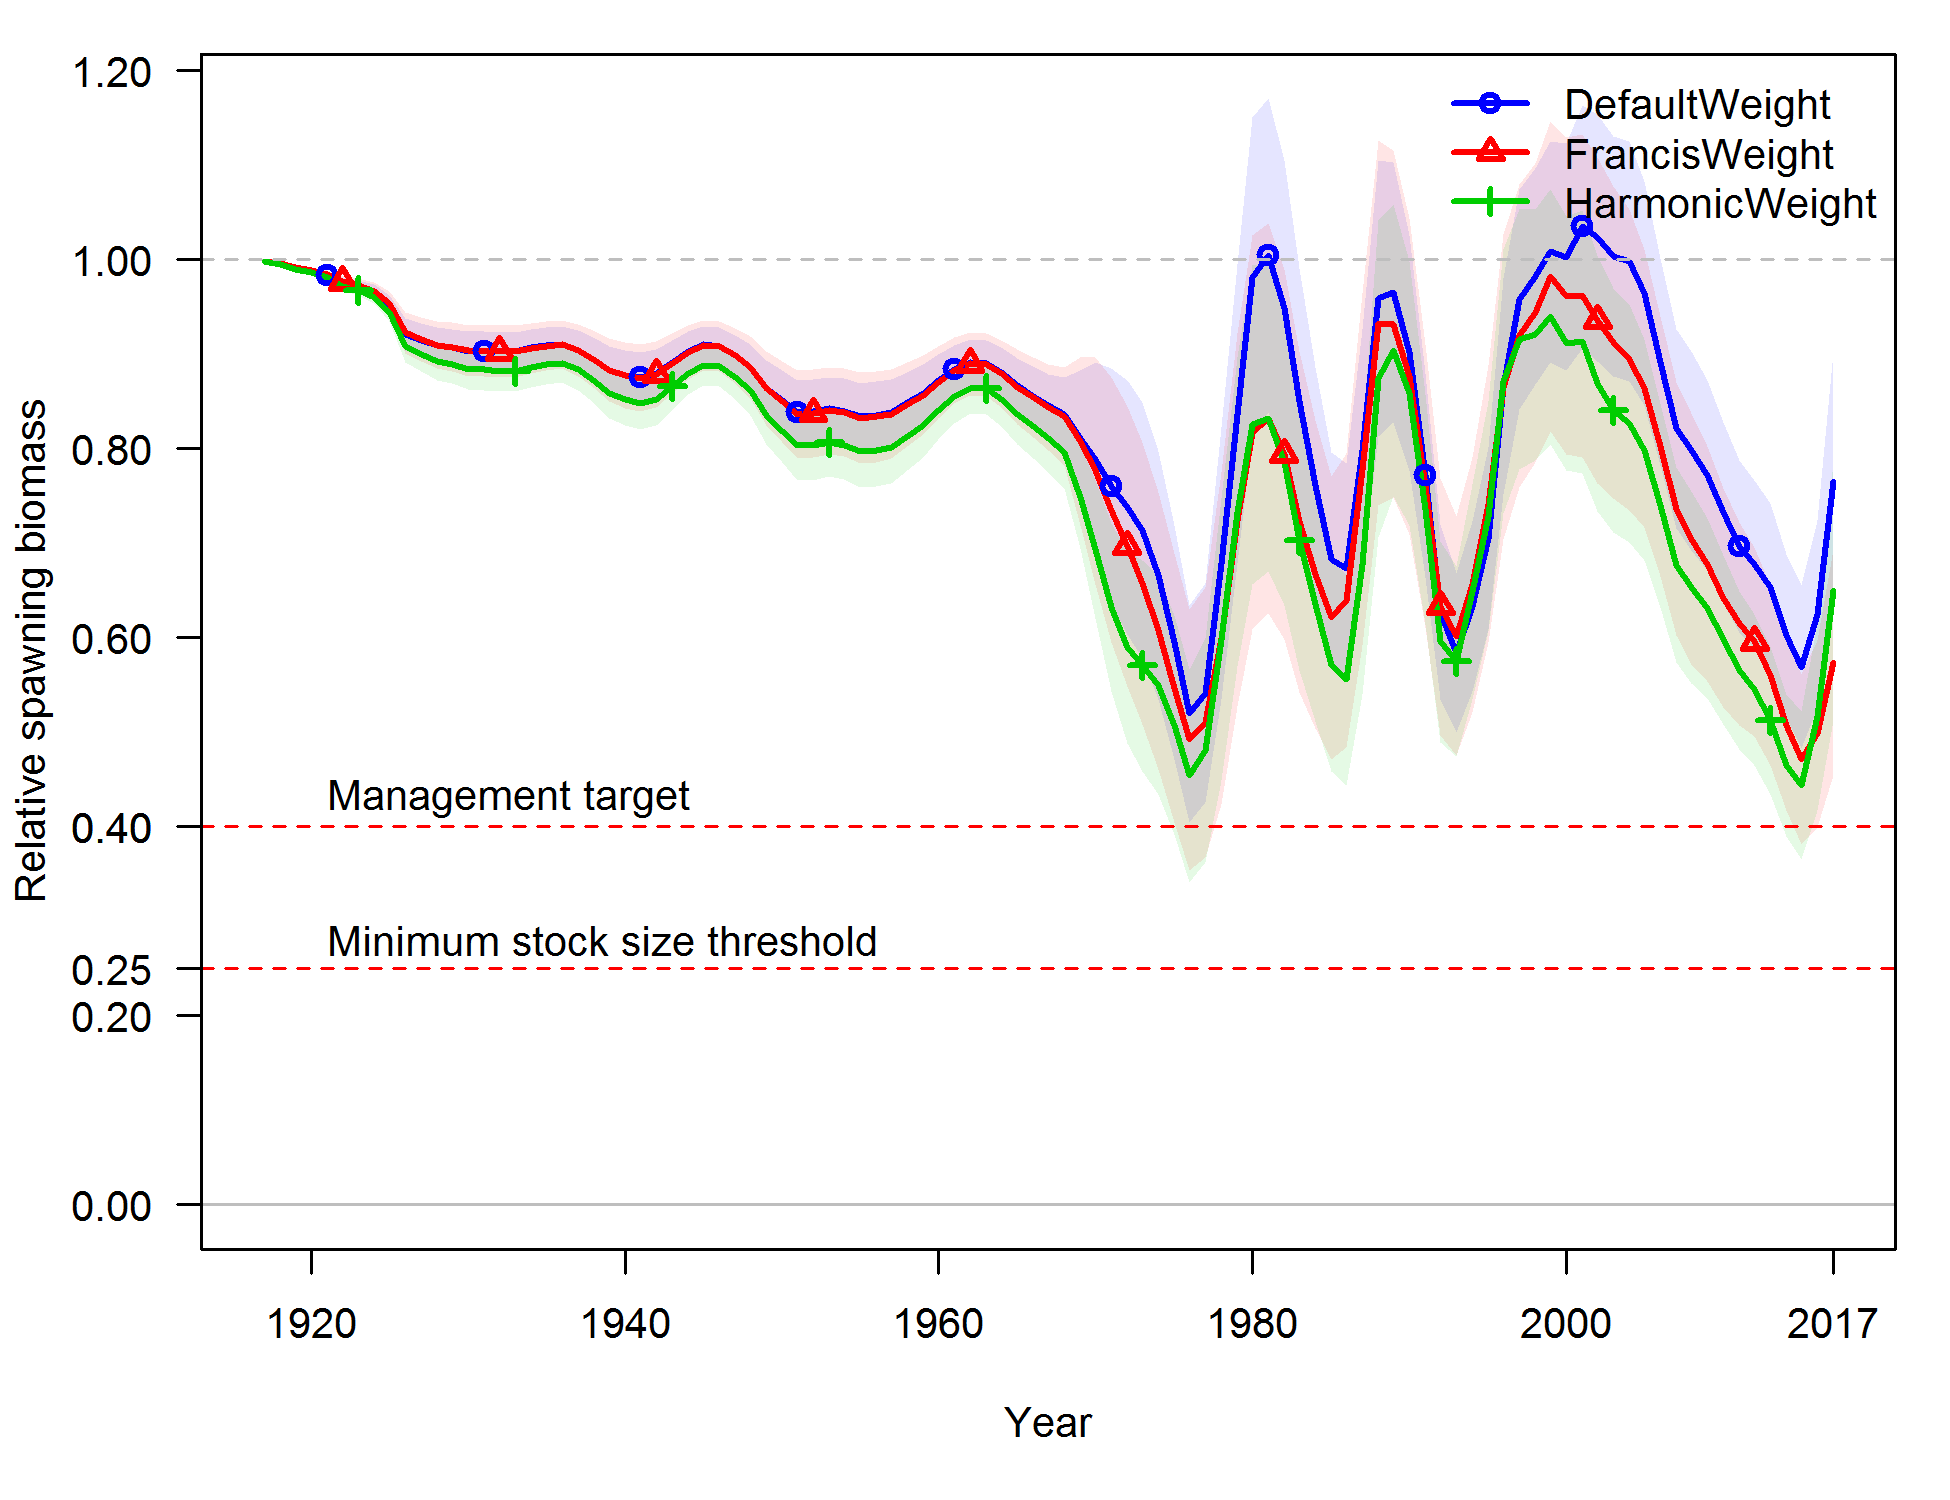
\includegraphics[height=4cm]{Figures/Data_weighting_Bratio.png} \endcol
\endcols

\end{frame}

\begin{frame}{Base Model Output (page 1)}

\begin{table}[ht]
\centering
\scalebox{0.5}{
\begin{tabular}{p{1.9in}p{.6in}p{.6in}p{.9in}p{.4in}p{.4in}p{2in}}
  \hline
Parameter & Value & Phase & Bounds & Status & SD & Prior (Exp.Val, SD) \\ 
  \hline
NatM\_p\_1\_Fem\_GP\_1 & 0.235 & -3 & (0.01, 1) &  &  & Log\_Norm (-1.3581, 0.438438) \\ 
  L\_at\_Amin\_Fem\_GP\_1 & 11.925 & 2 & (2, 30) & OK & 0.675 & None \\ 
  L\_at\_Amax\_Fem\_GP\_1 & 31.886 & 2 & (30, 50) & OK & 0.680 & None \\ 
  VonBert\_K\_Fem\_GP\_1 & 0.292 & 2 & (0.05, 0.5) & OK & 0.030 & None \\ 
  CV\_young\_Fem\_GP\_1 & 0.088 & 3 & (0.02, 0.5) & OK & 0.020 & None \\ 
  CV\_old\_Fem\_GP\_1 & 0.119 & 3 & (0.02, 0.75) & OK & 0.007 & None \\ 
  Wtlen\_1\_Fem & 0.000 & -3 & (-3, 3) &  &  & None \\ 
  Wtlen\_2\_Fem & 3.058 & -3 & (2, 4) &  &  & None \\ 
  Mat50\%\_Fem & 18.000 & -3 & (10, 30) &  &  & None \\ 
  Mat\_slope\_Fem & -1.200 & -3 & (-3, 3) &  &  & None \\ 
  Eggs/kg\_inter\_Fem & 1.000 & -3 & (-3, 3) &  &  & None \\ 
  Eggs/kg\_slope\_wt\_Fem & 0.000 & -3 & (-3, 3) &  &  & None \\ 
  NatM\_p\_1\_Mal\_GP\_1 & 0.000 & -2 & (-1, 1) &  &  & Normal (0, 99) \\ 
  L\_at\_Amin\_Mal\_GP\_1 & 0.000 & -2 & (-3, 3) &  &  & None \\ 
  L\_at\_Amax\_Mal\_GP\_1 & -0.143 & 2 & (-3, 3) & OK & 0.024 & None \\ 
  VonBert\_K\_Mal\_GP\_1 & -0.080 & 2 & (-3, 3) & OK & 0.144 & None \\ 
  CV\_young\_Mal\_GP\_1 & 1.318 & 3 & (-3, 3) & OK & 0.229 & None \\ 
  CV\_old\_Mal\_GP\_1 & -0.495 & 3 & (-3, 3) & OK & 0.121 & None \\ 
  Wtlen\_1\_Mal & 0.000 & -5 & (0, 1) &  &  & None \\ 
  Wtlen\_2\_Mal & 2.981 & -5 & (2, 4) &  &  & None \\ 
  CohortGrowDev & 1.000 & -1 & (1, 1) &  &  & None \\ 
  FracFemale\_GP\_1 & 0.500 & -4 & (0.000001, 0.999999) &  &  & None \\ 
  SR\_LN(R0) & 8.194 & 1 & (0, 31) & OK & 0.155 & None \\ 
  SR\_BH\_steep & 0.718 & -2 & (0.21, 0.99) &  &  & Full\_Beta (0.718, 0.158) \\ 
   \hline
\end{tabular}
}
\end{table}

\end{frame}

\begin{frame}{Pre-STAR Base Model Output (page 2)}

\begin{table}[ht]
\centering
\scalebox{0.5}{
\begin{tabular}{p{1.9in}p{.6in}p{.6in}p{.9in}p{.4in}p{.4in}p{2in}}
  \hline
Parameter & Value & Phase & Bounds & Status & SD & Prior (Exp.Val, SD) \\ 
  \hline
SR\_sigmaR & 0.600 & -2 & (0, 2) &  &  & None \\ 
  SR\_regime & 0.000 & -4 & (-5, 5) &  &  & None \\ 
  SR\_autocorr & 0.000 & -3 & (0, 0.5) &  &  & None \\ 
  LnQ\_base\_RecPR(4) & -6.847 & -1 & (-15, 15) &  &  & None \\ 
  Q\_extraSD\_RecPR(4) & 0.012 & 4 & (0.0001, 1) & OK & 0.022 & None \\ 
  LnQ\_base\_RecPC(5) & -11.255 & -1 & (-15, 15) &  &  & None \\ 
  Q\_extraSD\_RecPC(5) & 0.258 & 4 & (0.0001, 1) & OK & 0.047 & None \\ 
  LnQ\_base\_RecDD(6) & -10.578 & -1 & (-15, 15) &  &  & None \\ 
  Q\_extraSD\_RecDD(6) & 0.067 & 4 & (0.0001, 1) & OK & 0.043 & None \\ 
  LnQ\_base\_Sanitation(7) & -10.614 & -1 & (-15, 15) &  &  & None \\ 
  Q\_extraSD\_Sanitation(7) & 0.217 & 4 & (0.0001, 1) & OK & 0.047 & None \\ 
  LnQ\_base\_NWFSCTrawl(8) & -1.086 & -1 & (-15, 15) &  &  & None \\ 
  Q\_extraSD\_NWFSCTrawl(8) & 0.253 & 4 & (0.0001, 1) & OK & 0.145 & None \\ 
  LnQ\_base\_SCBSurvey(11) & -11.143 & -1 & (-15, 15) &  &  & None \\ 
  Q\_extraSD\_SCBSurvey(11) & 0.159 & 4 & (0.0001, 1) & OK & 0.139 & None \\ 
  LnQ\_base\_RecPCOBR(12) & -10.209 & -1 & (-15, 15) &  &  & None \\ 
  Q\_extraSD\_RecPCOBR(12) & 0.136 & 4 & (0.0001, 1) & OK & 0.046 & None \\ 
  SizeSel\_P1\_ComHL(1) & 24.436 & 5 & (13, 44) & OK & 1.166 & None \\ 
  SizeSel\_P2\_ComHL(1) & 15.000 & -3 & (-10, 16) &  &  & None \\ 
  SizeSel\_P3\_ComHL(1) & 2.119 & 5 & (-1, 10) & OK & 0.619 & None \\ 
  SizeSel\_P4\_ComHL(1) & 15.000 & -3 & (-1, 16) &  &  & None \\ 
  SizeSel\_P5\_ComHL(1) & -15.537 & 5 & (-25, -1) & OK & 128.790 & None \\ 
  SizeSel\_P6\_ComHL(1) & 10.000 & -3 & (-5, 11) &  &  & None \\ 
  SizeSel\_P1\_ComNet(2) & 44.000 & -5 & (13, 44) &  &  & None \\ 
  SizeSel\_P2\_ComNet(2) & 15.000 & -3 & (-10, 16) &  &  & None \\ 
  SizeSel\_P3\_ComNet(2) & 5.146 & 5 & (-1, 10) & OK & 0.234 & None \\ 
   \hline
\end{tabular}
}
\end{table}

\end{frame}

\begin{frame}{Pre-STAR Base Model Output (page 3)}

\begin{table}[ht]
\centering
\scalebox{0.5}{
\begin{tabular}{p{1.9in}p{.6in}p{.6in}p{.9in}p{.4in}p{.4in}p{2.1in}}
  \hline
Parameter & Value & Phase & Bounds & Status & SD & Prior (Exp.Val, SD) \\ 
  \hline
SizeSel\_P4\_ComNet(2) & 15.000 & -3 & (-1, 16) &  &  & None \\ 
  SizeSel\_P5\_ComNet(2) & -16.400 & 5 & (-25, -1) & OK & 119.734 & None \\ 
  SizeSel\_P6\_ComNet(2) & 10.000 & -3 & (-5, 11) &  &  & None \\ 
  SizeSel\_P1\_ComTrawl(3) & 1.000 & -2 & (1, 45) &  &  & None \\ 
  SizeSel\_P2\_ComTrawl(3) & 45.000 & -3 & (1, 45) &  &  & None \\ 
  SizeSel\_P1\_RecPR(4) & 42.043 & 5 & (13, 44) & OK & 2.423 & None \\ 
  SizeSel\_P2\_RecPR(4) & 15.000 & -3 & (-10, 16) &  &  & None \\ 
  SizeSel\_P3\_RecPR(4) & 4.572 & 5 & (-1, 10) & OK & 0.181 & None \\ 
  SizeSel\_P4\_RecPR(4) & 15.000 & -3 & (-1, 16) &  &  & None \\ 
  SizeSel\_P5\_RecPR(4) & -8.075 & 5 & (-25, -1) & OK & 0.792 & None \\ 
  SizeSel\_P6\_RecPR(4) & 10.000 & -3 & (-5, 11) &  &  & None \\ 
  SizeSel\_P1\_RecPC(5) & 37.769 & 5 & (13, 44) & OK & 1.567 & None \\ 
  SizeSel\_P2\_RecPC(5) & 15.000 & -3 & (-10, 16) &  &  & None \\ 
  SizeSel\_P3\_RecPC(5) & 4.609 & 5 & (-1, 10) & OK & 0.168 & None \\ 
  SizeSel\_P4\_RecPC(5) & 15.000 & -3 & (-1, 16) &  &  & None \\ 
  SizeSel\_P5\_RecPC(5) & -8.370 & 5 & (-25, -1) & OK & 2.026 & None \\ 
  SizeSel\_P6\_RecPC(5) & 10.000 & -3 & (-5, 11) &  &  & None \\ 
  SizeSel\_P1\_RecDD(6) & 22.469 & 5 & (13, 44) & OK & 0.091 & None \\ 
  SizeSel\_P2\_RecDD(6) & -11.207 & 4 & (-15, 16) & OK & 57.911 & None \\ 
  SizeSel\_P3\_RecDD(6) & 3.684 & 4 & (-1, 10) & OK & 0.490 & None \\ 
  SizeSel\_P4\_RecDD(6) & -10.915 & 4 & (-20, 5) & OK & 48.055 & None \\ 
  SizeSel\_P5\_RecDD(6) & -2.632 & 5 & (-25, 3) & OK & 0.390 & None \\ 
  SizeSel\_P6\_RecDD(6) & -2.583 & 4 & (-5, 11) & OK & 0.405 & None \\ 
  SizeSel\_P1\_Sanitation(7) & 23.678 & 4 & (13, 44) & OK & 0.487 & None \\ 
  SizeSel\_P2\_Sanitation(7) & 15.000 & -3 & (-10, 16) &  &  & None \\ 
   \hline
\end{tabular}
}
\end{table}

\end{frame}

\begin{frame}{Pre-STAR Base Model Output (page 4)}

\begin{table}[ht]
\centering
\scalebox{0.5}{
\begin{tabular}{p{2.5in}p{.6in}p{.6in}p{.9in}p{.4in}p{.4in}p{.4in}}
  \hline
Parameter & Value & Phase & Bounds & Status & SD & Prior (Exp.Val, SD) \\ 
  \hline
SizeSel\_P2\_Sanitation(7) & 15.000 & -3 & (-10, 16) &  &  & None \\ 
  SizeSel\_P3\_Sanitation(7) & 3.005 & 4 & (-1, 10) & OK & 0.158 & None \\ 
  SizeSel\_P4\_Sanitation(7) & 15.000 & -3 & (-1, 16) &  &  & None \\ 
  SizeSel\_P5\_Sanitation(7) & -4.582 & 4 & (-25, 5) & OK & 0.606 & None \\ 
  SizeSel\_P6\_Sanitation(7) & 10.000 & -3 & (-5, 11) &  &  & None \\ 
  SizeSel\_P1\_NWFSCTrawl(8) & 23.098 & 4 & (13, 44) & OK & 2.213 & None \\ 
  SizeSel\_P2\_NWFSCTrawl(8) & 15.000 & -3 & (-10, 16) &  &  & None \\ 
  SizeSel\_P3\_NWFSCTrawl(8) & 3.443 & 4 & (-1, 10) & OK & 0.616 & None \\ 
  SizeSel\_P4\_NWFSCTrawl(8) & 15.000 & -3 & (-1, 16) &  &  & None \\ 
  SizeSel\_P5\_NWFSCTrawl(8) & -12.730 & 4 & (-25, 5) & OK & 169.330 & None \\ 
  SizeSel\_P6\_NWFSCTrawl(8) & 10.000 & -3 & (-5, 11) &  &  & None \\ 
  SizeSel\_P1\_GillnetSurvey(9) & 1.000 & -2 & (1, 45) &  &  & None \\ 
  SizeSel\_P2\_GillnetSurvey(9) & 45.000 & -3 & (1, 45) &  &  & None \\ 
  SizeSel\_P1\_Impingement(10) & 18.012 & -3 & (13, 44) &  &  & None \\ 
  SizeSel\_P2\_Impingement(10) & -5.928 & 4 & (-15, 16) & OK & 27.411 & None \\ 
  SizeSel\_P3\_Impingement(10) & 2.137 & -4 & (-1, 10) &  &  & None \\ 
  SizeSel\_P4\_Impingement(10) & 2.701 & 4 & (-20, 5) & OK & 1.173 & None \\ 
  SizeSel\_P5\_Impingement(10) & 8.275 & -3 & (-25, 10) &  &  & None \\ 
  SizeSel\_P6\_Impingement(10) & -0.611 & 4 & (-5, 11) & OK & 0.476 & None \\ 
  SizeSel\_P1\_SCBSurvey(11) & 1.000 & -2 & (1, 45) &  &  & None \\ 
  SizeSel\_P2\_SCBSurvey(11) & 45.000 & -3 & (1, 45) &  &  & None \\ 
  SizeSel\_P1\_RecPCOBR(12) & 1.000 & -2 & (1, 45) &  &  & None \\ 
  SizeSel\_P2\_RecPCOBR(12) & 45.000 & -3 & (1, 45) &  &  & None \\ 
  SizeSel\_P1\_ComHL(1)\_BLK1repl\_1999 & 28.427 & 6 & (13, 44) & OK & 0.583 & None \\ 
  SizeSel\_P3\_ComHL(1)\_BLK1repl\_1999 & 2.029 & 6 & (-1, 10) & OK & 0.301 & None \\ 
  SizeSel\_P1\_ComNet(2)\_BLK1repl\_1999 & 44.000 & -6 & (13, 44) &  &  & None \\ 
   \hline
\end{tabular}
}
\end{table}

\end{frame}

\begin{frame}{Base Model Output}

\begin{table}[ht]
\centering
\scalebox{0.8}{
\begin{tabular}{lp{1in}p{1.2in}p{1in}p{1.2in}}
  \hline
Year & Spawning biomass (mt) & 95\% confidence interval & Estimated depletion & 95\% confidence interval \\ 
  \hline
2008 & 1144.50 & (654.46-1634.54) & 0.70 & (0.573-0.836) \\ 
  2009 & 1090.48 & (629.78-1551.18) & 0.67 & (0.55-0.793) \\ 
  2010 & 1029.33 & (597.2-1461.46) & 0.63 & (0.521-0.746) \\ 
  2011 & 980.13 & (571.79-1388.47) & 0.60 & (0.5-0.707) \\ 
  2012 & 943.55 & (553.81-1333.3) & 0.58 & (0.485-0.677) \\ 
  2013 & 890.08 & (518.85-1261.32) & 0.55 & (0.456-0.64) \\ 
  2014 & 810.22 & (462.86-1157.59) & 0.50 & (0.41-0.587) \\ 
  2015 & 746.23 & (412.08-1080.38) & 0.46 & (0.371-0.548) \\ 
  2016 & 774.81 & (426.28-1123.35) & 0.48 & (0.381-0.572) \\ 
  2017 & 882.46 & (484.21-1280.71) & 0.54 & (0.43-0.657) \\ 
   \hline
\end{tabular}
}
\end{table}

\end{frame}

\begin{frame}{Base Model Output}

\begin{table}[ht]
\centering
\scalebox{0.7}{
\begin{tabular}{p{.8in}p{.8in}p{.8in}p{.8in}p{.8in}p{.8in}}
  \hline
Year & OFL & ABC & ACL & ACT & Total Catch \\ 
  \hline
\textbf{2007} & 219 &  & 175 &  & 139.583 \\ 
  \textbf{2008} & 219 &  & 175 &  & 103.887 \\ 
  \textbf{2009} & 175 &  & 175 &  & 113.318 \\ 
  \textbf{2010} & 155 &  & 155 &  & 105.968 \\ 
  \textbf{2011} & 141 & 135 & 135 &  & 105.215 \\ 
  \textbf{2012} & 132 & 126 & 126 &  & 120.008 \\ 
  \textbf{2013} & 126 & 120 & 120 &  & 115.142 \\ 
  \textbf{2014} & 122 & 117 & 117 &  & 123.822 \\ 
  \textbf{2015} & 119 & 114 & 114 &  & 83.8908 \\ 
  \textbf{2016} & 117 & 111 & 111 &  & 74.1613 \\ 
  \textbf{2017} & 289 & 264 & 150 & 110 & - \\ 
  \textbf{2018} & 278 & 254 & 150 & 110 & - \\ 
   \hline
\end{tabular}
}
\end{table}

\end{frame}

\section{Uncertainty}\label{uncertainty}

\begin{frame}{Sensitivities}

Sensitivities to Likelihood Components and Model Specification
\begincols
 \begincol{.5\textwidth} \includegraphics{Figures/Sensitivity_All.pdf}
\endcol
 \begincol{.5\textwidth}

\begin{itemize}
\item Remove fleets, only one index, or length composition only
\item Sensitivity relative to the base model
\item Boxes are the 95\% CI from the base model
\item Metrics
\begin{itemize}
\item $SB_0$ Population scale
\item $SB_{2017}$ Population scale
\item $SB_{2017}/SB_{0}$ Depletion/Population status
\item $MSY_{SPR50\%}$ Yield/Productivity/scale
\end{itemize}
\end{itemize}

\endcol
\endcols

\end{frame}

\begin{frame}{Sensitivities - All}

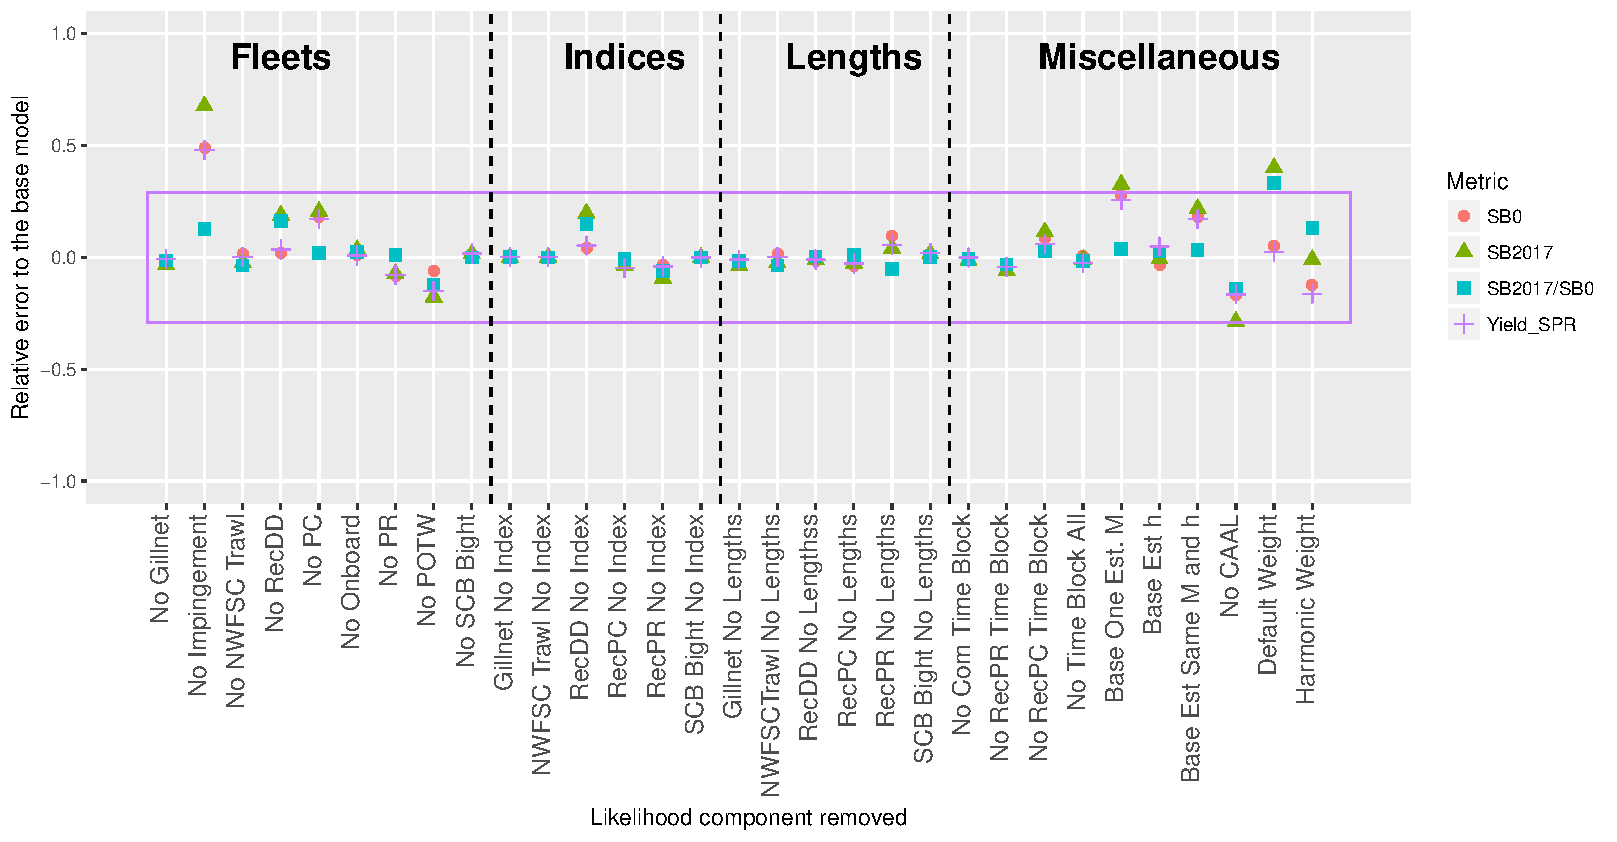
\includegraphics{Figures/Sensitivity_Yield.pdf}

\end{frame}

\end{document}
